\documentclass[12pt, a4paper]{article}

% If you can't see cyrillic letters in R-studio choose
% File-Reopen with encoding
% utf8 is the preferred encoding


%%%%%%%%%%%%%%%%%%%%%%%  Загрузка пакетов  %%%%%%%%%%%%%%%%%%%%%%%%%%%%%%%%%%
% кусок от урсса
%\usepackage[60x90,headers,11pt]{format}

%\textheight=494pt%
%\textwidth=322pt%
%
%\oddsidemargin=0pt%
%\evensidemargin=0pt
%\topmargin=-1pt \headsep=14pt \headheight=22pt \voffset=-28pt
%\hoffset=-50pt


\clubpenalty=10000
\widowpenalty=10000

%\overfullrule=5pt
%\hfuzz=1.5mm
%\baselineskip=12pt plus 0.18pt minus 0.1pt


%\pagestyle{headings}
% конец куска от урсса



% специальная версия для knitr'а. Исключает graphicx

%\usepackage{showkeys} % показывать метки в готовом pdf

\usepackage{etex} % расширение классического tex
% в частности позволяет подгружать гораздо больше пакетов, чем мы и займёмся далее

%\usepackage{mathtext} % русские буквы в формулах? (и без неё работает)
% Например, $x_{\text{один}}$


\usepackage{verbatim} % для многострочных комментариев
\usepackage{makeidx} % для создания предметных указателей



\usepackage{setspace}
\usepackage{amsmath, amsfonts, amssymb, amsthm}
\usepackage{mathrsfs} % sudo yum install texlive-rsfs
\usepackage{dsfont} % sudo yum install texlive-doublestroke
\usepackage{array, multicol, multirow, bigstrut} % sudo yum install texlive-multirow
\usepackage{indentfirst} % установка отступа в первом абзаце главы




\usepackage{bm}
\usepackage{bbm} % шрифт с двойными буквами
%\usepackage[perpage]{footmisc}

\usepackage{dcolumn} % центрирование по разделителю для apsrtable

% создание гиперссылок в pdf
\usepackage[unicode, colorlinks=true, urlcolor=blue, hyperindex, breaklinks]{hyperref}


\usepackage{microtype} % свешиваем пунктуацию
% теперь знаки пунктуации могут вылезать за правую границу текста, при этом текст выглядит ровнее


\usepackage{textcomp}  % Чтобы в формулах можно было русские буквы писать через \text{}

% размер листа бумаги
%\usepackage[paperwidth=145mm,paperheight=215mm,
%height=182mm,width=113mm,top=20mm,includefoot]%{geometry}
\usepackage[paper=a4paper, top=15mm, bottom=13.5mm, left=16.5mm, right=13.5mm, includefoot]{geometry}

\usepackage{xcolor}

% \usepackage[pdftex]{graphicx} % для вставки графики, убрано, т.к. knitr похоже сам добавляет

\usepackage{float, longtable}
\usepackage{soulutf8}

\usepackage{enumitem} % дополнительные плюшки для списков
%  например \begin{enumerate}[resume] позволяет продолжить нумерацию в новом списке

\usepackage{mathtools}
\usepackage{cancel, xspace} % sudo yum install texlive-cancel

% \usepackage{minted} % display program code with syntax highlighting
% требует установки pygments и python

\usepackage{numprint} % sudo yum install texlive-numprint
\npthousandsep{,}\npthousandthpartsep{}\npdecimalsign{.}


\usepackage{subfigure} % для создания нескольких рисунков внутри одного

\usepackage{tikz, pgfplots} % язык для рисования графики из latex'a
\usetikzlibrary{trees} % tikz-прибамбас для рисовки деревьев
\usepackage{tikz-qtree} % альтернативный tikz-прибамбас для рисовки деревьев
\usetikzlibrary{arrows} % tikz-прибамбас для рисовки стрелочек подлиннее

\usepackage{todonotes} % для вставки в документ заметок о том, что осталось сделать
% \todo{Здесь надо коэффициенты исправить}
% \missingfigure{Здесь будет Последний день Помпеи}
% \listoftodos --- печатает все поставленные \todo'шки



\usepackage{booktabs} %  красивые таблицы
% заповеди из докупентации:
% 1. Не используйте вертикальные линни
% 2. Не используйте двойные линии
% 3. Единицы измерения - в шапку таблицы
% 4. Не сокращайте .1 вместо 0.1
% 5. Повторяющееся значение повторяйте, а не говорите "то же"


\usepackage{fontspec} % что-то про шрифты?
\usepackage{polyglossia} % русификация xelatex

\setmainlanguage{russian}
\setotherlanguages{english}

% download "Linux Libertine" fonts:
% http://www.linuxlibertine.org/index.php?id=91&L=1
\setmainfont{Linux Libertine O} % or Helvetica, Arial, Cambria
% why do we need \newfontfamily:
% http://tex.stackexchange.com/questions/91507/
\newfontfamily{\cyrillicfonttt}{Linux Libertine O}

\AddEnumerateCounter{\asbuk}{\russian@alph}{щ} % для списков с русскими буквами
\setlist[enumerate, 2]{label=\asbuk*),ref=\asbuk*}


%\usepackage{asymptote} % пакет для рисовки графики, должен идти после graphics
% но мы переходим на tikz :)

%\usepackage{sagetex} % для интеграции с Sage (вероятно тоже должен идти после graphics)

% metapost создает упрощенные eps файлы, которые можно напрямую включать в pdf
% эта группа команд декларирует, что файлы будут этого упрощенного формата
% если metapost не используется, то этот блок не нужен
\usepackage{ifpdf} % для определения, запускается ли pdflatex или просто латех
\ifpdf
	\DeclareGraphicsRule{*}{mps}{*}{}
\fi
%%%%%%%%%%%%%%%%%%%%%%%%%%%%%%%%%%%%%%%%%%%%%%%%%%%%%%%%%%%%%%%%%%%%%%




%%%%%%%%%%%%%%%%%%%%%%%  ПАРАМЕТРЫ  %%%%%%%%%%%%%%%%%%%%%%%%%%%%%%%%%%
\setstretch{1}                          % Межстрочный интервал
\flushbottom                            % Эта команда заставляет LaTeX чуть растягивать строки, чтобы получить идеально прямоугольную страницу
\righthyphenmin=2                       % Разрешение переноса двух и более символов
%\pagestyle{plain}                       % Нумерация страниц снизу по центру.
%\widowpenalty=300                     % Небольшое наказание за вдовствующую строку (одна строка абзаца на этой странице, остальное --- на следующей)
%\clubpenalty=3000                     % Приличное наказание за сиротствующую строку (омерзительно висящая одинокая строка в начале страницы)
\setlength{\parindent}{1.5em}           % Красная строка.
%\captiondelim{. }
\setlength{\topsep}{0pt}
%%%%%%%%%%%%%%%%%%%%%%%%%%%%%%%%%%%%%%%%%%%%%%%%%%%%%%%%%%%%%%%%%%%%%%



%%%%%%%% Это окружение, которое выравнивает по центру без отступа, как у простого center
\newenvironment{center*}{%
  \setlength\topsep{0pt}
  \setlength\parskip{0pt}
  \begin{center}
}{%
  \end{center}
}
%%%%%%%%%%%%%%%%%%%%%%%%%%%%%%%%%%%%%%%%%%%%%%%%%%%%%%%%%%%%%%%%%%%%%%


%%%%%%%%%%%%%%%%%%%%%%%%%%% Правила переноса  слов
\hyphenation{ }
%%%%%%%%%%%%%%%%%%%%%%%%%%%%%%%%%%%%%%%%%%%%%%%%%%%%%%%%%%%%%%%%%%%%%%

\emergencystretch=2em


% DEFS
\def \mbf{\mathbf}
\def \msf{\mathsf}
\def \mbb{\mathbb}
\def \tbf{\textbf}
\def \tsf{\textsf}
\def \ttt{\texttt}
\def \tbb{\textbb}

\def \wh{\widehat}
\def \wt{\widetilde}
\def \ni{\noindent}
\def \ol{\overline}
\def \cd{\cdot}
\def \fr{\frac}
\def \bs{\backslash}
\def \lims{\limits}
\DeclareMathOperator{\dist}{dist}
\DeclareMathOperator{\VC}{VCdim}
\DeclareMathOperator{\card}{card}
\DeclareMathOperator{\sign}{sign}
\DeclareMathOperator{\sgn}{sign}
\DeclareMathOperator{\Tr}{\mbf{Tr}}
\DeclareMathOperator{\tr}{tr}


\def \xfs{(x_1,\ldots,x_{n-1})}
\DeclareMathOperator*{\argmin}{arg\,min}
\DeclareMathOperator*{\amn}{arg\,min}
\DeclareMathOperator*{\amx}{arg\,max}
\DeclareMathOperator{\trace}{tr}
\DeclareMathOperator{\rk}{rk}


\DeclareMathOperator{\Corr}{Corr}
\DeclareMathOperator{\sCorr}{sCorr}
\DeclareMathOperator{\sCov}{sCov}
\DeclareMathOperator{\sVar}{sVar}

\DeclareMathOperator{\Cov}{Cov}
\DeclareMathOperator{\Var}{Var}
\DeclareMathOperator{\corr}{Corr}
\DeclareMathOperator{\cov}{Cov}
\DeclareMathOperator{\var}{Var}
\DeclareMathOperator{\bin}{Bin}
\DeclareMathOperator{\Bin}{Bin}
\DeclareMathOperator{\rang}{rang}
\DeclareMathOperator*{\plim}{plim}
\DeclareMathOperator{\MSE}{MSE}

\newcommand{\norm}[1]{\left\lVert#1\right\rVert}

\providecommand{\iff}{\Leftrightarrow}
\providecommand{\hence}{\Rightarrow}

\def \ti{\tilde}
\def \wti{\widetilde}

\def \mA{\mathcal{A}}
\def \mB{\mathcal{B}}
\def \mC{\mathcal{C}}
\def \mE{\mathcal{E}}
\def \mF{\mathcal{F}}
\def \mH{\mathcal{H}}
\def \mL{\mathcal{L}}
\def \mN{\mathcal{N}}
\def \mU{\mathcal{U}}
\def \mV{\mathcal{V}}
\def \mW{\mathcal{W}}


\def \R{\mbb R}
\def \N{\mbb N}
\def \Z{\mbb Z}
\def \P{\mbb{P}}
\def \p{\mbb{P}}
\newcommand{\E}{\mathbb{E}}
\def \D{\msf{D}}
\def \I{\mbf{I}}

\def \QQ{\mbb Q}
\def \RR{\mbb R}
\def \NN{\mbb N}
\def \ZZ{\mbb Z}
\def \PP{\mbb P}


\def \a{\alpha}
\def \b{\beta}
\def \t{\tau}
\def \dt{\delta}
\newcommand{\e}{\varepsilon}
\def \ga{\gamma}
\def \kp{\varkappa}
\def \la{\lambda}
\def \sg{\sigma}
\def \sgm{\sigma}
\def \tt{\theta}
\def \ve{\varepsilon}
\def \Dt{\Delta}
\def \La{\Lambda}
\def \Sgm{\Sigma}
\def \Sg{\Sigma}
\def \Tt{\Theta}
\def \Om{\Omega}
\def \om{\omega}

%\newcommand{\p}{\partial}

\def \ni{\noindent}
\def \lq{\glqq}
\def \rq{\grqq}
\def \lbr{\linebreak}
\def \vsi{\vspace{0.1cm}}
\def \vsii{\vspace{0.2cm}}
\def \vsiii{\vspace{0.3cm}}
\def \vsiv{\vspace{0.4cm}}
\def \vsv{\vspace{0.5cm}}
\def \vsvi{\vspace{0.6cm}}
\def \vsvii{\vspace{0.7cm}}
\def \vsviii{\vspace{0.8cm}}
\def \vsix{\vspace{0.9cm}}
\def \VSI{\vspace{1cm}}
\def \VSII{\vspace{2cm}}
\def \VSIII{\vspace{3cm}}

\newcommand{\bls}[1]{\boldsymbol{#1}}
\newcommand{\bsA}{\boldsymbol{A}}
\newcommand{\bsH}{\boldsymbol{H}}
\newcommand{\bsI}{\boldsymbol{I}}
\newcommand{\bsP}{\boldsymbol{P}}
\newcommand{\bsR}{\boldsymbol{R}}
\newcommand{\bsS}{\boldsymbol{S}}
\newcommand{\bsX}{\boldsymbol{X}}
\newcommand{\bsY}{\boldsymbol{Y}}
\newcommand{\bsZ}{\boldsymbol{Z}}
\newcommand{\bse}{\boldsymbol{e}}
\newcommand{\bsq}{\boldsymbol{q}}
\newcommand{\bsy}{\boldsymbol{y}}
\newcommand{\bsbeta}{\boldsymbol{\beta}}
\newcommand{\fish}{\mathrm{F}}
\newcommand{\Fish}{\mathrm{F}}
\renewcommand{\phi}{\varphi}
\newcommand{\ind}{\mathds{1}}
\newcommand{\inds}[1]{\mathds{1}_{\{#1\}}}
\renewcommand{\to}{\rightarrow}
\newcommand{\sumin}{\sum\limits_{i=1}^n}
\newcommand{\ofbr}[1]{\bigl( \{ #1 \} \bigr)}     % Например, вероятность события. Большие круглые, нормальные фигурные скобки вокруг аргумента
\newcommand{\Ofbr}[1]{\Bigl( \bigl\{ #1 \bigr\} \Bigr)} % Например, вероятность события. Больше больших круглые, большие фигурные скобки вокруг аргумента
\newcommand{\oeq}{{}\textcircled{\raisebox{-0.4pt}{{}={}}}{}} % Равно в кружке
\newcommand{\og}{\textcircled{\raisebox{-0.4pt}{>}}}  % Знак больше в кружке

% вместо горизонтальной делаем косую черточку в нестрогих неравенствах
\renewcommand{\le}{\leqslant}
\renewcommand{\ge}{\geqslant}
\renewcommand{\leq}{\leqslant}
\renewcommand{\geq}{\geqslant}


\newcommand{\figb}[1]{\bigl\{ #1  \bigr\}} % большие фигурные скобки вокруг аргумента
\newcommand{\figB}[1]{\Bigl\{ #1  \Bigr\}} % Больше больших фигурные скобки вокруг аргумента
\newcommand{\parb}[1]{\bigl( #1  \bigr)}   % большие скобки вокруг аргумента
\newcommand{\parB}[1]{\Bigl( #1  \Bigr)}   % Больше больших круглые скобки вокруг аргумента
\newcommand{\parbb}[1]{\biggl( #1  \biggr)} % большие-большие круглые скобки вокруг аргумента
\newcommand{\br}[1]{\left( #1  \right)}    % круглые скобки, подгоняемые по размеру аргумента
\newcommand{\fbr}[1]{\left\{ #1  \right\}} % фигурные скобки, подгоняемые по размеру аргумента
\newcommand{\eqdef}{\mathrel{\stackrel{\rm def}=}} % знак равно по определению
\newcommand{\const}{\mathrm{const}}        % const прямым начертанием
\newcommand{\zdt}[1]{\textit{#1}}
\newcommand{\ENG}[1]{\foreignlanguage{british}{#1}}
\newcommand{\ENGs}{\selectlanguage{british}}
\newcommand{\RUSs}{\selectlanguage{russian}}
\newcommand{\iid}{\text{i.\hspace{1pt}i.\hspace{1pt}d.}}

\newdimen\theoremskip
\theoremskip=0pt
\newenvironment{note}{\par\vskip\theoremskip\textbf{Замечание.\xspace}}{\par\vskip\theoremskip}
\newenvironment{hint}{\par\vskip\theoremskip\textbf{Подсказка.\xspace}}{\par\vskip\theoremskip}
\newenvironment{ist}{\par\vskip\theoremskip Источник:\xspace}{\par\vskip\theoremskip}

\newcommand*{\tabvrulel}[1]{\multicolumn{1}{|c}{#1}}
\newcommand*{\tabvruler}[1]{\multicolumn{1}{c|}{#1}}

\newcommand{\II}{{\fontencoding{X2}\selectfont\CYRII}}   % I десятеричное (английская i неуместна)
\newcommand{\ii}{{\fontencoding{X2}\selectfont\cyrii}}   % i десятеричное
\newcommand{\EE}{{\fontencoding{X2}\selectfont\CYRYAT}}  % ЯТЬ
\newcommand{\ee}{{\fontencoding{X2}\selectfont\cyryat}}  % ять
\newcommand{\FF}{{\fontencoding{X2}\selectfont\CYROTLD}} % ФИТА
\newcommand{\ff}{{\fontencoding{X2}\selectfont\cyrotld}} % фита
\newcommand{\YY}{{\fontencoding{X2}\selectfont\CYRIZH}}  % ИЖИЦА
\newcommand{\yy}{{\fontencoding{X2}\selectfont\cyrizh}}  % ижица

%%%%%%%%%%%%%%%%%%%%% Определение разрядки разреженного текста и задание красивых многоточий
\sodef\so{}{.15em}{1em plus1em}{.3em plus.05em minus.05em}
\newcommand{\ldotst}{\so{...}}
\newcommand{\ldotsq}{\so{?\hbox{\hspace{-0.61ex}}..}}
\newcommand{\ldotse}{\so{!..}}
%%%%%%%%%%%%%%%%%%%%%%%%%%%%%%%%%%%%%%%%%%%%%%%%%%%%%%%%%%%%%%%%%%%%%%

%%%%%%%%%%%%%%%%%%%%%%%%%%%%% Команда для переноса символов бинарных операций
\def\hm#1{#1\nobreak\discretionary{}{\hbox{$#1$}}{}}
%%%%%%%%%%%%%%%%%%%%%%%%%%%%%%%%%%%%%%%%%%%%%%%%%%%%%%%%%%%%%%%%%%%%%%

%\setlist[enumerate,1]{label=\arabic*., ref=\arabic*, partopsep=0pt plus 2pt, topsep=0pt plus 1.5pt,itemsep=0pt plus .5pt,parsep=0pt plus .5pt}
%\setlist[itemize,1]{partopsep=0pt plus 2pt, topsep=0pt plus 1.5pt,itemsep=0pt plus .5pt,parsep=0pt plus .5pt}

% Эти парни затем, если вдруг не захочется управлять списками из-под уютненького enumitem
% или если будет жизненно важно, чтобы в списках были именно русские буквы.
%\setlength{\partopsep}{0pt plus 3pt}
%\setlength{\topsep}{0pt plus 2pt}
%\setlength{\itemsep}{0 plus 1pt}
%\setlength{\parsep}{0 plus 1pt}

%на всякий случай пока есть
%теоремы без нумерации и имени
%\newtheorem*{theor}{Теорема}

%"Определения","Замечания"
%и "Гипотезы" не нумеруются
%\newtheorem*{defin}{Определение}
%\newtheorem*{rem}{Замечание}
%\newtheorem*{conj}{Гипотеза}

%"Теоремы" и "Леммы" нумеруются
%по главам и согласованно м/у собой
%\newtheorem{theorem}{Теорема}
%\newtheorem{lemma}[theorem]{Лемма}

% Утверждения нумеруются по главам
% независимо от Лемм и Теорем
%\newtheorem{prop}{Утверждение}
%\newtheorem{cor}{Следствие}

\input{emetrix_preamble}


\usepackage{minted}

\usepackage[bibencoding = auto,
backend = biber,
sorting = none,
style=alphabetic]{biblatex}

\addbibresource{probability_pro.bib}

\def \RR{\mathbb{R}}
\def \cN{\mathcal{N}}
\newcommand{\Lin}{\mathcal{L}in}
\newcommand{\Linp}{\Lin^{\perp}}

\title{Заметки к семинарам по вероятностям}
\author{Винни-Пух}
\date{\today}


% делаем короче интервал в списках
\setlength{\itemsep}{0pt}
\setlength{\parskip}{0pt}
\setlength{\parsep}{0pt}


\DeclareMathOperator{\Med}{Med}


\usepackage{answers}

%\newtheorem{problem}{Задача}
%\numberwithin{problem}{section}

\Newassociation{sol}{solution}{solution_file}
% sol --- имя окружения внутри задач
% solution --- имя окружения внутри solution_file
% solution_file --- имя файла в который будет идти запись решений
% можно изменить далее по ходу
\Opensolutionfile{solution_file}[all_solutions]
% в квадратных скобках фактическое имя файла



% магия для автоматических гиперссылок задача-решение
\newlist{myenum}{enumerate}{3}
% \newcounter{problem}[chapter] % нумерация задач внутри глав
\newcounter{problem}[section]

\newenvironment{problem}%
{%
\refstepcounter{problem}%
%  hyperlink to solution
     \hypertarget{problem:{\thesection.\theproblem}}{} % нумерация внутри глав
     % \hypertarget{problem:{\theproblem}}{}
     \Writetofile{solution_file}{\protect\hypertarget{soln:\thesection.\theproblem}{}}
     %\Writetofile{solution_file}{\protect\hypertarget{soln:\theproblem}{}}
     \begin{myenum}[label=\bfseries\protect\hyperlink{soln:\thesection.\theproblem}{\thesection.\theproblem},ref=\thesection.\theproblem]
     % \begin{myenum}[label=\bfseries\protect\hyperlink{soln:\theproblem}{\theproblem},ref=\theproblem]
     \item%
    }%
    {%
    \end{myenum}}
% для гиперссылок обратно надо переопределять окружение
% это происходит непосредственно перед подключением файла с решениями




\begin{document}

% \maketitle % ставим сюда название, автора и время создания

\section{Вперёд, в рукопашную!}


Минитеория:

\begin{enumerate}
\item \url{http://bdemeshev.github.io/pr201/} или \url{http://pokrovka11.wordpress.com}
\item Константы. Cтрочные английские буквы, $a$, $x$, $z$.
\item События. Заглавные английский буквы начала алфавита $A$, $B$, $C$, $D$. Вероятность $\P(A)$.
\item Случайные величины. Заглавные английский буквы конца алфавита $X$, $Y$, $W$, $Z$. Математическое ожидание $\E(X)$.
\end{enumerate}

Задачи:

\begin{problem}
В вазе пять неотличимых с виду конфет.
Две без ореха и три — с орехом. Маша ест конфеты выбирая их наугад до тех пор,
пока не съест первую конфету с орехом. Обозначим $X$ — число съеденных конфет.
Найдите $\P(X=2)$, $\P(X>1)$, $\E(X)$


\begin{sol}
  $\P(X=1)=3/5$, $\P(X=2)=3/10$, $\P(X=3)=1/10$, $\E(X)=1.5$
\end{sol}
\end{problem}

\begin{problem}
В коробке находится четыре внешне одинаковые лампочки,  две из них исправны.
Лампочки извлекают из коробки по одной до тех пор, пока не будут извлечены обе исправные.
\begin{enumerate}
\item Какова вероятность того, что опыт закончится извлечением трёх лампочек?
\item Каково ожидаемое количество извлеченных лампочек?
\end{enumerate}

\begin{sol}
\end{sol}
\end{problem}

\begin{problem}
Маша подкидывает монетку. Если в первый раз монетка выпала орлом, то Маша подкидывает монетку ещё один раз,
если решкой — то ещё два раза. Больше Маша монетку не подкидывает!
Пусть $X$ — количество выпавших орлов.

Найдите вероятности $\P(X=0)$, $\P(X=1)$, \ldots и ожидание $\E(X)$.

\begin{sol}
\end{sol}
\end{problem}

\begin{problem}
Две команды равной силы играют в волейбол до трёх побед одной из них,
не обязательно подряд. Ничья невозможна. Из-за равенства сил будем считать,
что вероятность победы каждой равна $0.5$. Величина $N$ — количество сыгранных партий.

Составьте табличку возможных значений $N$ с их вероятностями.

Найдите $\P(N \text{ — чётное})$, $\E(N)$


\begin{sol}
   N 3 4 5

  2/8 3/8 3/8
\end{sol}
\end{problem}

\begin{problem}
 Какова вероятность того, что у 30 человек не будет ни одного
совпадения дней рождений? Сколько человек должно собраться, чтобы вероятность совпадения дней рождения превысила $1/2$? Сколько в среднем человек должно войти в комнату, чтобы впервые произошло совпадения дней рождения?

\begin{sol}
\end{sol}
\end{problem}

\begin{problem}
 Саша и Маша по очереди подбрасывают кубик до первой шестёрки. Посуду будет
мыть тот, кто первым выбросит шестерку. Маша бросает кубик первой.
Какова вероятность того, что посуду будет мыть Маша? Сколько в среднем раз они будут бросать кубик?

\begin{sol}
 $6/11$, $6$
\end{sol}
\end{problem}

\begin{problem}
 Неправильную монетку с вероятностью «орла» равной $0.7$ подбрасывают до первого «орла».
 Чему равно среднее количество подбрасываний?  Орлов? Решек? Какова вероятность чётного числа бросков? Как изменятся ответы, если вероятность орла будет равна $p$?


\begin{sol}
  $N$ — количество подбрасываний, $G$ — количество орлов, $R$ — решек

  $\E(N)=10/7$, $\E(G)=1$, $\E(R)=10/7-1=3/7$

  Для вероятности чётного числа бросков можно сложить ряд или составить уравнение.
  Если выпала решка, то в продолжении игры мы хотим получить нечётное количество бросков.
  \[
     v = 0.7 \cdot 0 + 0.3 \cdot (1-v)
  \]
\end{sol}
\end{problem}

\begin{problem}
 Вы играете в следующую игру. Кубик подкидывается неограниченное число раз.
 Если на кубике выпадает 1, 2 или 3, то соответствующее количество монет добавляется на кон.
 Если выпадает 4 или 5, то игра оканчивается и Вы получаете сумму, лежащую на кону.
 Если выпадает 6, то игра оканчивается, а Вы не получаете ничего. Изначально на кону лежит ноль рублей.
\begin{enumerate}
\item Какова вероятность того, что игра рано или поздно закончится выпадением 6-ки?
\item Какова ожидаемая продолжительность игры?
\item Чему равен ожидаемый выигрыш?
\item Чему равен ожидаемый выигрыш, если изначально на кону лежит 100 рублей?
\item Изменим изначальное условие: если выпадает 5, то сумма на кону сгорает, а игра продолжается.
Чему будет равен средний выигрыш в новую игру?
\end{enumerate}

\begin{sol}
\end{sol}
\end{problem}

\begin{problem}
 Саша и Маша подкидывают монетку до тех пор, пока не выпадет
последовательность РОО или ОOР. Если игра закончится выпадением
РОО, то выигрывает Саша, если ОOР, то — Маша. Случайная величина $X$ — общее количество подбрасываний, $Y$ — количество выпавших решек.
\begin{enumerate}
\item У кого какие шансы выиграть?
\item $\P(X=4)$, $\P(Y=1)$, $\E(X)$, $\E(Y)$
\item Решите аналогичную задачу для ОРО и ООР.
\end{enumerate}

\begin{sol}
  у Саши 3/4
\end{sol}
\end{problem}

\begin{problem}
 Вася подкидывает кубик до тех пор, пока на кубике не выпадет единица, или пока он сам не скажет «Стоп». Вася получает столько рублей, сколько выпало на кубике при последнем броске. Вася хочет максимизировать свой ожидаемый выигрыш.
\begin{enumerate}
\item Как выглядит оптимальная стратегия? Чему равен ожидаемый выигрыш при использовании оптимальной стратегии?
\item Какова средняя продолжительность игры при использовании оптимальной стратегии?
\item Как выглядит оптимальная стратегия и чему равен ожидаемый выигрыш, если за каждое
подбрасывание Вася платит 35 копеек?
\end{enumerate}

\begin{sol}
  стоп на 4-5-6 или стоп на 5-6
\end{sol}
\end{problem}

\begin{problem}
 Саша и Маша решили, что будут заводить новых детей до тех пор,
 пока в их семье не будут дети обоих полов. Обозначим $X$ — количество детей в их семье.
 Найдите $\P(X=4)$, $\E(X)$.

\begin{sol}
  $\P(X=4)=1/8$, $\E(X)=3$
\end{sol}
\end{problem}


\begin{problem}
В каждой вершине треугольника по ёжику. Каждую минуту с вероятностью $0.5$ каждый ежик
независимо от других двигается по часовой стрелке, с вероятностью
$0.5$ — против часовой стрелки.
Обозначим $T$ — время до встречи всех ежей в одной вершине.

\begin{enumerate}
  \item Найдите $\P(T=1)$, $\P(T=2)$, $\P(T=3)$, $\E(T)$.
  \item Как изменятся ответы, если вероятность движения по часовой стрелке равна $p$?
\end{enumerate}

\begin{sol}
\end{sol}
\end{problem}


\section{Хочу ещё задач!}


\begin{problem}
Наугад из четырех тузов разных мастей выбираются два.
$\P(\text{они будут разного цвета})$?

\begin{sol}
\end{sol}
\end{problem}
\begin{problem}
 События $A$  и  $B$ несовместны, то есть не могут произойти одновременно. Известны вероятности $\P(A)=0.3$, $\P(B)=0.4$. Найдите\footnote{Событие $A^c$ — это событие противоположное событию $A$, иногда обозначается $\bar{A}$} $\P(A^{c} \cap B^{c} )$.

\begin{sol}
\end{sol}
\end{problem}
\begin{problem}
 Вероятность $\P(A)=0.3$,  $\P(B)=0.8$. В каких пределах может лежать $\P(A\cap B)$?

\begin{sol}
\end{sol}
\end{problem}
\begin{problem}
 Множество исходов $\Omega =\left\{a,b,c\right\}$, $\P(\left\{a,b\right\})=0,8$,
$\P(\{b,c\})=0,7$. Найдите $\P(\{a\})$, $\P(\{b\})$, $\P(\{c\})$

\begin{sol}
\end{sol}
\end{problem}
\begin{problem}
 «Amoeba». A population starts with a single amoeba. For this one and for the generations thereafter, there is a probability of 3/4 that an individual amoeba will split to create two amoebas, and a 1/4 probability that it will die out without producing offspring. Let the random variable $X$ be the number of generations before the death of all the amoebas. Find the probabilities $\P(X=2)$, $\P(X=3)$, $\P(X=\infty)$


\begin{sol}
\end{sol}
\end{problem}
\begin{problem}
 Вася нажимает на пульте телевизора кнопку «On-Off» 100 раз
подряд. Пульт старый, поэтому в первый раз кнопка срабатывает с
вероятностью $\frac{1}{2}$, затем вероятность срабатывания падает.
Какова вероятность того, что после всех нажатий телевизор будет
включен, если сейчас он выключен?


\begin{sol}
  1/2
\end{sol}
\end{problem}
\begin{problem}
 Suppose the probability to get a head when throwing an unfair coin is $p$,
 what's the expected number of throwings in order to get two consecutive heads?
 The expected number of tails?


\begin{sol}
  $\E(X)=0.25\cdot 2 + 0.5\cdot (\E(X)+1)+0.25\cdot (\E(X)+2)$

  $\E(Y)=0.25\cdot 0 + 0.5\cdot (\E(Y)+1)+0.25\cdot (\E(Y)+1)$
\end{sol}
\end{problem}

\begin{problem}
 Вам предложена следующая игра. Изначально на кону 0 рублей. Раз за разом подбрасывается правильная монетка. Если она выпадает орлом, то казино добавляет на кон 100 рублей. Если монетка выпадает решкой, то все деньги, лежащие на кону, казино забирает себе, а Вы получаете красную карточку. Игра прекращается либо когда Вы получаете третью красную карточку, либо в любой момент времени до этого по Вашему выбору. Если Вы решили остановить игру до получения трех красных карточек, то Ваш выигрыш равен сумме на кону. При получении третьей красной карточки игра заканчивается и Вы не получаете ничего. Вы заинтересованы в максимальном среднем выигрыше.
\begin{enumerate}
\item Как выглядит оптимальная стратегия, если только что была получена вторая красная карточка? Чему равен средний выигрыш?
\item Как выглядит оптимальная стратегия, если только что была получена первая красная карточка?
\item Как выглядит оптимальная стратегия в исходной игре? Чему равен средний выигрыш?
\end{enumerate}

\begin{sol}
стратегия 1: говорить стоп, если на кону 200 рублей вне зависимости от числа набранных красных карточек

 стратегия 2: если нет красных карточек или одна, то останавливаться при 200 рублях, а при двух карточках останавливаться на 100 рублях.
\end{sol}
\end{problem}

\begin{problem}
 Есть три комнаты. В первой из них лежит сыр. Если мышка
попадает в первую комнату, то она находит сыр через одну минуту.
Если мышка попадает во вторую комнату, то она ищет сыр две минуты
и покидает комнату. Если мышка попадает в третью комнату, то она
ищет сыр три минуты и покидает комнату. Покинув комнату, мышка
выходит в коридор и выбирает новую комнату наугад, например, может
зайти в одну и ту же. Сейчас мышка в коридоре. Сколько времени ей
в среднем потребуется, чтобы найти сыр?

\begin{sol}
\end{sol}
\end{problem}

\begin{problem}
Илье Муромцу предстоит дорога к камню. От камня начинаются ещё три дороги.
Каждая из тех дорог снова оканчивается камнем. И от каждого камня начинаются ещё три дороги.
И каждые те три дороги оканчиваются камнем\ldots И так далее до бесконечности.
На каждой дороге живёт трёхголовый Змей Горыныч.
Каждый Змей Горыныч бодрствует независимо от других с вероятностью (хм, Вы не поверите!) одна третья.
У Василисы Премудрой существует Чудо-Карта, на которой видно,
какие Змеи Горынычи бодрствуют, а какие — нет.

Какова вероятность того,
что Василиса Премудрая сможет найти на карте
бесконечный жизненный путь Ильи Муромца проходящий исключительно мимо спящих Змеев Горынычей?

\begin{sol}
\end{sol}
\end{problem}

\begin{problem}
 У Пети — монетка, выпадающая орлом с вероятностью $ p\in (0;1) $.
 У Васи — с вероятностью $1/2$. Они одновременно подбрасывают свои монетки до тех пор,
 пока у них не окажется набранным одинаковое количество орлов.
 В частности, они останавливаются после первого подбрасывания,
 если оно дало одинаковые результаты. Сколько в среднем раз им придётся подбросить монетку?

\begin{sol}
\end{sol}
\end{problem}
\begin{problem}
 Треугольник с вершинами $(0;0)$, $(2;0)$ и $(1;1)$. Внутри него случайным образом выбирается точка, $X$ -- абсцисса точки. Найдите $\P(X>1)$, $\P(X\in [0.5;1])$, $\E(X)$

\begin{sol}
\end{sol}
\end{problem}
\begin{problem}
 Треугольник с вершинами $(0;0)$, $(2;0)$ и $(2;1)$. Внутри него случайным образом выбирается точка, $X$ -- абсцисса точки. Найдите $\P(X>1)$, $\P(X\in [0.5;1])$. Что больше, $\E(X)$ или 1?


\begin{sol}
\end{sol}
\end{problem}
\begin{problem}
 Исследовательница Мишель подкидывает игральный кубик неограниченное количество раз и складывает выпадающие количества очков.
\begin{enumerate}
\item Чему примерно равна вероятность того, что однажды сумма в точности будет равна 123456789?
\item Чему точно равна указанная вероятность?
\end{enumerate}

\begin{sol}
\end{sol}
\end{problem}
\begin{problem}
 Упрямая исследовательница Мишель подбрасывает монетку до тех пор, пока количество орлов не окажется в точности равным удвоенному количеству решек. Монетка выпадает орлом с вероятностью $p$. Какова вероятность того, что Мишель будет подкидывать монетку вечно?

\begin{sol}
\end{sol}
\end{problem}


\begin{problem}
 Исследовательница Мишель хочет встать утром с правой ноги с вероятностью $1/\sqrt{2}$, и с левой с вероятностью $1 - 1/\sqrt{2}$. Однако для проведения случайных экспериментов у неё есть только одна правильная монетка. Как с помощью правильной монетки ей добиться цели?

\begin{sol}
\end{sol}
\end{problem}


\begin{problem}
Докажите каждое равенство словами, без использования факториалов.
Затем обобщите каждое равенство, добавив туда $n$, $k$ и суммы.
\begin{enumerate}
  \item $\binom{10}{7} = \binom{10}{3}$
  \item $\binom{10}{3} + \binom{10}{4} = \binom{11}{4}$
  \item $\binom{4}{0} + \binom{4}{1} + \binom{4}{2} + \binom{4}{3} + \binom{4}{4} = 2^4$
  \item $ 4 \binom{10}{4} = 10 \binom{9}{3}$
  \item $\binom{10}{3}\binom{7}{2} = \binom{10}{2}\binom{8}{3}$
  \item $1\cdot \binom{5}{1} + 2\cdot \binom{5}{2} + 3\cdot \binom{5}{3} + 4\cdot\binom{5}{4} + 5\cdot \binom{5}{5} = 5 \cdot 2^4$
  \item $\binom{2}{2} + \binom{3}{2} + \binom{4}{2} + \binom{5}{2} = \binom{6}{3}$
  \item $\binom{4}{0}\binom{5}{3} + \binom{4}{1}\binom{5}{2} +  \binom{4}{2}\binom{5}{1} +  \binom{4}{3}\binom{5}{0} =\binom{9}{3}$
  \item $\binom{4}{0}^2 + \binom{4}{1}^2 + \binom{4}{2}^2 + \binom{4}{3}^2 + \binom{4}{4}^2 = \binom{8}{4}$
\end{enumerate}

\begin{sol}
\begin{enumerate}
  \item Выбрать три, чтобы взять, или выбрать семь, чтобы не взять.
  \item Число дорог с 11 ходами вниз и 4 вправо равно сумму числа дорог.
  \item Число всех подмножеств в множестве из 4-х элементов.
  \item Из 10 человек хотим выбрать одного лидера и 3-х помощников.
  \item Из 10 человек хотим выбрать 3-х орлов и 2-х слонов.
  \item Число всех подмножеств с одним лидером в множестве из 5-ти элементов.
\end{enumerate}

\end{sol}
\end{problem}


\begin{problem}
Объясните каждую интерпретацию словами, без использования факториалов.
\begin{enumerate}
  \item $\binom{10}{4}$ — количество строк из 4 единиц и 6 нулей
  \item $\binom{7}{4}$ — количество строк из 4 единиц и 6 нулей, в которых единицы не идут подряд
  \item $\binom{10}{4}$ — число способов раздать 4 яблока 10 людям, не дав никому больше одного
  \item $\binom{13}{4}$ — число способов раздать 4 яблока 10 людям
\end{enumerate}

\begin{sol}
\end{sol}
\end{problem}


\section{К чёрту условности!}


\begin{problem}
  Имеется три монетки. Две «правильных» и одна — с
«орлами» по обеим сторонам. Петя выбирает одну монетку наугад и
подкидывает её два раза. Оба раза выпадает «орел». Какова
условная вероятность того, что монетка «неправильная»?

\begin{sol}
  $\P(A\mid B)=\frac{\P(A \cap B)}{\P(B)}= \frac{1/3}{1/6+1/3}=2/3$
\end{sol}
\end{problem}

\begin{problem}
  Два охотника одновременно выстрелили в одну утку. Первый попадает с
вероятностью 0.4, второй — с вероятностью 0.7 независимо от первого.
\begin{enumerate}
\item Какова вероятность того, что в утку попала ровно одна пуля?
\item  Какова условная вероятность того, что утка была убита первым
охотником, если в утку попала ровно одна пуля?
\end{enumerate}

\begin{sol}
  $A$ — первый охотник попал в утку, $B$ — в утку попала ровно одна пуля

  $\P(A \mid B)=\frac{\P(A \cap B)}{\P(B)}= \frac{0.4 \cdot 0.3 }{0.4\cdot 0.3 + 0.6\cdot 0.7}=2/9$
\end{sol}
\end{problem}

\begin{problem}
 Кубик подбрасывается два раза. Найдите вероятность получить
сумму равную 8, если при первом броске выпало 3.

\begin{sol}
  $\P(A \mid B)=1/6$
\end{sol}
\end{problem}

\begin{problem}
Игрок получает 13 карт из колоды в 52 карты.
Какова вероятность, что у него как минимум два туза, если
известно, что у него есть хотя бы один туз?
Какова вероятность того, что у него как минимум два туза, если
известно, что у него есть туз пик?

\begin{sol}
Обозначим: $X$ — количество попавшихся тузов, $S$ — количество попавшихся тузов пик.

\[
\P(X = 2) = \frac{C_4^2 C_{48}^{11}}{C_{52}^{13}}
\]
$\P(X\geq 2 \mid X\geq 1)=\frac{\P(X \geq 2)}{\P(X \geq 1)}= \approx 0.37$


Можно представить, что мы берём первые 13 карт из случайно перемешанной колоды.
Поэтому вероятность того, что туз пик попадет на одно из этих 13-и мест равна:
\[
\P(S=1) = \frac{13}{52}
\]

Далее,
\[
\P(X\geq 2 \mid S = 1) = \frac{\P(S=1, X\geq 2)}{\P(S=1)}
\]

Ищем вероятность в числителе. Есть много способов, один из:
\[
\P(S=1, X\geq 2) = \P(S=1) - \P(S=1, X=1) = \frac{13}{52} - \frac{1\cdot C_{48}^{12}}{C_{52}^{13}}
\]

Итого, $\P(X \geq 2 \mid S = 1) \approx 0.56$.

\end{sol}
\end{problem}
\begin{problem}
 В урне 7 красных, 5 желтых и 11 белых шаров. Два шара
выбирают наугад. Какова вероятность, что это красный и белый, если
известно, что они разного цвета?

\begin{sol}
  $\P(A \mid B)=\frac{\P(A \cap B)}{\P(B)}= \frac{7\cdot 11 /C_{7+5+11}^2}{(7\cdot 11+5\cdot 11 + 7\cdot 5) /C_{7+5+11}^2 }$
\end{sol}
\end{problem}

\begin{problem}
  В урне 5 белых и 11 черных шаров. Два шара извлекаются по
очереди. Какова вероятность того, что второй шар будет черным?
Какова вероятность того, что первый шар — белый, если известно,
что второй шар — черный?

\begin{sol}
  $B$ — событие, второй — черный, $\P(B)=11/16$

  $\P(A \mid B)=\P(A \cap B)/\P(B)=\frac{\frac{5}{16}\frac{11}{15}}{11/16}$
\end{sol}
\end{problem}

\begin{problem}
 Примерно 4\% коров заражены «коровьим бешенством».  Имеется тест, который дает ошибочный результат с вероятностью 0,1. Судя по тесту, новая партия мяса заражена. Какова вероятность того, что она действительно заражена?

\begin{sol}
  $A$ — партия мяса заражена, $B$ — партия мяса по тесту заражена

  $\P(A \mid B)=\P(A \cap B)/\P(B)=\frac{0.04\cdot 0.9}{0.04\cdot 0.9+0.96\cdot 0.1}\approx 0.27$
\end{sol}
\end{problem}

\begin{problem}
 В школе три девятых класса, «А», «Б» и «В», одинаковые по
численности. В «А» классе 30\% обожают учителя географии, в «Б»
классе — 40\% и в «В» классе — 70\%. Девятиклассник Петя обожает
учителя географии. Какова вероятность того, что он из «Б» класса?

\begin{sol}
  $A$ — Петя из Б класса, $B$ — Петя обожает географию

  $\P(A \mid B)=\P(A \cap B)/\P(B)=\frac{0.4/3}{0.3/3+0.4/3+0.7/3}=2/7$
\end{sol}
\end{problem}

\begin{problem}
 Ген карих глаз доминирует ген синих. Следовательно, у носителя пары bb
глаза синие, а у носителя пар BB и Bb — карие. У диплоидных
организмов (а мы такие :)) одна аллель наследуется от папы, а одна
— от мамы. В семье у кареглазых родителей два сына — кареглазый и
синеглазый. Кареглазый женился на синеглазой девушке. Какова
вероятность рождения у них синеглазого ребенка?

\begin{sol}
  $1/3$
\end{sol}
\end{problem}

\begin{problem}
  Из колоды в 52 карты извлекается одна карта наугад. Являются
ли события «извлечен туз» и «извлечена пика» независимыми?

\begin{sol}
  да
\end{sol}
\end{problem}

\begin{problem}
  Из колоды в 52 карты извлекаются по очереди две карты
наугад. Являются ли события «первая карта — туз» и «вторая
карта — туз» независимыми?

\begin{sol}
  нет, $(4/52)\cdot (3/51)=\P(A\cap B) \neq \P(A)\cdot \P(B)=(4/52)^2$
\end{sol}
\end{problem}

\begin{problem}
  Известно, что $\P(A)=0,3$, $\P(B)=0,4$, $\P(C)=0,5$. События
$A$ и $B$ несовместны, события $A$ и $C$ независимы и
$\P(B|C)=0,1$. Найдите $\P(A\cup B\cup C)$.

\begin{sol}
\end{sol}
\end{problem}

\begin{problem}
 У тети Маши — двое детей, один старше другого. Предположим, что вероятности рождения мальчика и девочки равны и не зависят от дня недели, а пол первого и второго ребенка независимы. Для каждой из четырех ситуаций найдите условную вероятность того, что у тёти Маши есть дети обоих полов.
\begin{enumerate}
\item Известно, что хотя бы один ребенок — мальчик.
\item Тетя Маша наугад выбирает одного своего
ребенка и посылает к тете Оле, вернуть учебник по теории
вероятностей. Это оказывается мальчик.
\item Известно, что старший ребенок — мальчик.
\item На вопрос: «А правда ли тетя Маша, что у вас есть сын, родившийся в пятницу?» тётя Маша ответила: «Да».
\end{enumerate}

\begin{sol}
$ 2/3 $, $1/2$, $ 1/2 $, $ 14/27 $
\end{sol}
\end{problem}

\section{Use Julia/R/python/\ldots or die!}


\begin{problem}
 Самая простая. Случайная величина $N$ имеет пуассоновское распределение с $\lambda=2$. С помощью симуляций оцените $\E(N^3)$, $\P(N \geq 4)$, $\P(N \geq 10 \mid N \geq 5)$, $\E(N \mid N \geq 5)$. Функция \verb|rpois| может помочь :)

\begin{sol}
\end{sol}
\end{problem}
\begin{problem}
 Случайные величины $X_1$, \ldots, $X_5$ имеют равномерное распределение на отрезке $[0;1]$ и независимы. С помощью симуляций оцените $\P(\min\{X_1,\ldots,X_5\}>0.2)$, $\P(\min\{X_1,\ldots,X_5\}>0.2 \mid X_1+X_2 < 0.5)$, $\E(\min\{X_1,\ldots,X_5\})$, $\E(\min\{X_1,\ldots,X_5\} \mid X_1+X_2 < 0.5)$

\begin{sol}
\end{sol}
\end{problem}
\begin{problem}
 Случайные величины $X_1$, $X_2$ независимы и обе имеют биномиальное распределение с параметрами $n=16$, $p=0.7$. Величина $Y$ задана формулой $Y=X_1/(1+X_2)$. С помощью симуляций оцените $\P(Y>0.5)$, $\E(Y)$, $\P(Y>0.5 \mid X_1>10 )$, $\E(Y \mid X_1 > 10)$. Функция \verb|rbinom| в помощь!

\begin{sol}
\end{sol}
\end{problem}
\begin{problem}
 В колоде 52 карты. Мы вытаскиваем карты из колоды до первого туза, пусть $X$ — количество вытянутых карт. С помощью симуляций оцените $\E(X^2)$, $\P(X>10)$, $\P(X>5 \mid X<15)$, $\E(X^2 \mid X<15)$

\begin{sol}
\end{sol}
\end{problem}
\begin{problem}
 Иван Федорович Крузенштерн случайным образом с возможностью повторов выбирает 10 натуральных чисел от 1 до 100. Пусть $X$ — минимум этих чисел, а $Y$ — максимум. С помощью симуляций оцените $\P(Y>3X)$, $\E(XY)$, $\P(Y>3X \mid Y<X^2)$, $\E(XY \mid Y<X^2)$

\begin{sol}
\end{sol}
\end{problem}


\newpage
\section{Эф большое и эф малое}

Минитеория:


\begin{enumerate}
\item $F_X(t) = \P(X \leq t)$
\item  $F(t) = \int_{-\infty}^ t f(a) \, da$, $f(t)=F'(t)$.
\end{enumerate}


Задачи:

\begin{problem}
 Функция плотности случайной величины $X$ равна $5$ при $x=7$. Найдите примерно вероятность того, что $X$ попадёт в отрезок $[7;7.001]$.

\begin{sol}
\end{sol}
\end{problem}
\begin{problem}
 Случайная величина $X$ имеет функцию плотности $f$. С помощью $o(\Delta)$ и $f(x)$ запишите вероятность $\P(X\in [x;x+\Delta])$.

\begin{sol}
\end{sol}
\end{problem}
\begin{problem}
 Величина $X$ распределена на отрезке $[0;1]$ и на нём имеет функцию плотности $f(t)=3t^2$. Найдите функции плотности и функции распределения величин $Y=\ln X$, $Z=X^2$, $W=(X-0.5)^2$.

\begin{sol}
\end{sol}
\end{problem}
\begin{problem}
 Может ли функция плотности принимать значение больше 2015? Может ли предел $\lim_{x\to\infty} f(x)$ не равняться нулю?

\begin{sol}
\end{sol}
\end{problem}
\begin{problem}
 Функция плотности случайной величины  $X$ имеет
вид:
\[
f(t)=
\begin{cases}
  \frac{3}{16}t^2,t\in [-2;2] \\
  0, t\notin [-2;2]
\end{cases}
\]
Найдите:
\begin{enumerate}
\item $\P(X>1)$, $\E(X)$, $\E(X^{2})$, $\Var(X)$, $\sigma_{X}$
\item $\E(X|X>1)$, $\E(X^{2}|X>1)$, $\Var(X|X>1)$
\item Функцию распределения случайной величины $X$
\item Медиану величины $X$, 40\%-ую квантиль величины $X$
\end{enumerate}

\begin{sol}
\end{sol}
\end{problem}
\begin{problem}
 Функция плотности случайной величины  $X$ имеет
вид:
\[
f(t)=
\begin{cases}
  t/8, t\in [0;4] \\
  0, t\notin [0;4]
\end{cases}
\]
Найдите:
\begin{enumerate}
\item $\P(X>1)$, $\E(X)$, $\E(X^{2})$, $\Var(X)$, $\sigma_{X}$
\item $\E(X|X>1)$, $\E(X^{2}|X>1)$, $\Var(X|X>1)$
\item Функцию распределения случайной величины $X$
\item Медиану величины $X$, 40\%-ую квантиль величины $X$
\end{enumerate}

\begin{sol}
\end{sol}
\end{problem}
\begin{problem}
 Величина $X$ распределена на отрезке $[0;2]$ и имеет на нём функцию распределения $F(x)=x^2/4$. Найдите $\P(X\in [1;1.5])$, $\P(X<1)$, $F(-5)$, $F(10)$, функцию плотности величины $X$

\begin{sol}
\end{sol}
\end{problem}
\begin{problem}
 Если возможно, найдите функцию распределения и функцию плотности величины $X$ принимающей значения $1$, $2$, $3$ и $4$ с вероятностями $0.1$, $0.2$, $0.3$ и $0.4$ соответственно.


\begin{sol}
\end{sol}
\end{problem}
\begin{problem}
 Величина $X$ равномерна на отрезке $[-2;1]$, а величина $Y$ — это расстояние от числа $X$ до числа $(-1)$. Найдите фукнцию плотности $Y$, $\E(Y)$.

\begin{sol}
\end{sol}
\end{problem}
\begin{problem}
 Глафира случайным образом равномерно выбирает случайную внутри треугольника с вершинами $(0;0)$, $(0;2)$ и $(3;3)$. Пусть $X$ и $Y$ — абсцисса и ордината выбранной точки. Найдите функцию плотности $X$, функцию плотности $Y$.

\begin{sol}
\end{sol}
\end{problem}
\begin{problem}
  Прямой убыток от пожара в миллионах рублей равномерно распределен на
$[0;1]$. Если убыток оказывается больше 0.7, то страховая компания выплачивает компенсацию 0.7.
\begin{enumerate}
\item Найдите функцию распределения потерь от пожара.
\item Чему равны средние потери?
\end{enumerate}

\begin{sol}
\end{sol}
\end{problem}
\begin{problem}
 Пусть $X$ — неотрицательная случайная величина с функцией плотности $f(t)$
и $\E(X)<\infty$. При каком $c$ функция $g(t)=c\cdot t \cdot f(t)$ также
будет функцией плотности?

\begin{sol}
при $c=1/\E(X)$
\end{sol}
\end{problem}
\begin{problem}
 Завтрашняя цена акции — случайная величина с функцией плотности  $f(x)=\frac{3}{4}
\max \left\{x(2-x),0\right\}$.
\begin{enumerate}
\item Постройте график функции плотности
\item Найдите функцию распределения Васиного дохода, средний доход и дисперсию дохода, если:
\begin{enumerate}
\item У Васи есть 10 акций
\item У Васи есть опцион-пут, дающий ему право продать акции по цене 1.2 рубля
\item У Васи есть опцион-колл, дающий ему право купить акции по цене 1 рубль
\end{enumerate}
\end{enumerate}


\begin{sol}
\end{sol}
\end{problem}
\begin{problem}
 В соревнованиях по прыжкам в длину участвовали $n$ спортсменов. Результаты их прыжков, величины $X_i$, независимы и одинаково распределены с функцией плотности $f$ и функцией распределения $F$.
\begin{enumerate}
\item Найдите функцию распределения и функцию плотности длины наилучшего прыжка
\item Найдите функцию распределения и функцию плотности длины наихудшего прыжка
\item Найдите вероятность того, что Сидоров и Петров прыгнули меньше чем на $t$ метров, Иванов прыгнул от $t$ до $t+\Delta$ метров, а остальные прыгнули больше, чем на $t$ метров.
\item Найдите функцию распределения и функцию плотности длины прыжка бронзового призёра соревнований
\end{enumerate}

\begin{sol}
\end{sol}
\end{problem}
\begin{problem}
 Светофор попеременно горит пешеходу то 40 секунд зелёным, то 60 секунд — красным. Законопослушный Вася Бубликов подходит к светофору в случайный момент времени. Пусть $X$ — время ожидания до возможности перейти дорогу.
\begin{enumerate}
 \item Найдите функцию распределения величины $X$ и постройте её график
 \item Найдите $\E(X)$ и $\Var(X)$
\end{enumerate}


\begin{sol}
\end{sol}
\end{problem}
\begin{problem}
 Большой Адронный Коллайдер запускают ровно в полночь. Оставшееся время до Конца Света — случайная величина $X$ распределенная равномерно от 0 до 16 часов. Когда произойдет Конец Света, механические часы остановятся и будут показывать время $Y$.
\begin{enumerate}
\item Найдите $\P(Y<2)$
\item Постройте функцию плотности величины $Y$
\item Найдите $\E(Y)$, $\Var(Y)$
\item Найдите $\Cov(X,Y)$
\end{enumerate}

\begin{sol}
\end{sol}
\end{problem}


\newpage
\section{Рождение распределений}


\begin{problem}
«Всякая вещь — или есть, или нет»

Как справедливо заметил исследователь Винни-Пух, всякая вещь — или есть, или нет. Рассмотрим случайную величину $V$, равную единице, если вещь — есть, и нулю иначе. Допустим вероятность того, что вещь есть равна $0.7$.
\begin{enumerate}
  \item Составьте табличку со значениями $V$ и их вероятностями;
  \item Найдите $\E(V)$ и $\Var(V)$;
  \item Если возможно, нарисуйте функцию распределения и функцию плотности $V$;
  \item Найдите $\E(V)$ и $\Var(V)$, если вероятность того, что вещь — есть равна параметру $p$.
\end{enumerate}

Определение. Случайная величина $V$ имеет распределение Бернулли с параметром $p$.

\begin{sol}

\end{sol}
\end{problem}

\begin{problem}
Винни-Пух и Пятачок играют в Пустяки (Poohsticks). Каждую партию Винни-Пух выигрывает с вероятностью $p=0.7$. Всего они сыграли $n=10$ партий. Пусть $X$ — количество партий, выигранных Винни-Пухом.
\begin{enumerate}
  \item Объясните правила игры Пустяки;
  \item Найдите $\P(X=0)$, $\P(X=10)$, $\P(X=4)$, $\P(X=k)$;
  \item Представьте $X$ в виде суммы 10 случайных величин с распределением Бернулли, поясните, что означает каждое слагаемое.
  \item Найдите $\E(X)$ и $\Var(X)$. Здесь без доказательства можно пользоваться тем, что для независимых величин $R$ и $S$ дисперсия раскладывается в сумму $\Var(R+S)=\Var(R) + \Var(S)$;
  \item Найдите $\P(X=k)$, $\E(X)$ и $\Var(X)$ для произвольных $p$, $n$;
\end{enumerate}

Определение. Случайная величина $X$ имеет биномиальное распределение с параметрами $n$ и $p$;
\begin{sol}
\end{sol}
\end{problem}



\begin{problem}
«Ну не то, чтобы совсем не попал\ldots»

Храбрый Пятачок спешит с ружьём на помощь зависшему исследователю Винни-Пуху. При каждом выстреле Пятачок попадает в шарик с вероятностью $p=0.7$ независимо от предыдущих выстрелов. Стреляет Пятачок до первого попадания. Пусть $X$ — это количество выстрелов, $Y$ — количество промахов по шарику\footnote{или попаданий по исследователю Винни-Пуху}.

\begin{enumerate}
  \item Найдите $\P(X=2)$, $\P(X=3)$, $\P(X=k)$.
  \item Терпения Винни-Пуха хватает на 5 промахов Пятачка. Какова вероятность того, что терпения Винни-Пуха не хватит?
  \item Найдите $\P(Y=2)$, $\P(Y=3)$, $\P(Y=k)$.
  \item С помощью метода первого шага найдите $\E(X)$ и $\E(X^2)$;
  \item Найдите $\Var(X)$
  \item Каким соотношением связаны $X$ и $Y$?
  %\item С помощью метода первого шага найдите $\E(Y)$ и $\E(Y^2)$;
  \item Как связаны $\E(X)$ и $\E(Y)$, $\Var(X)$ и $\Var(Y)$?
  \item Чему будут равны $\P(X=k)$, $\E(X)$ и $\Var(X)$, если при отдельном выстреле Пятачок попадает с вероятностью $p$?
  %\item Чему будут равны $\P(Y=k)$, $\E(Y)$ и $\Var(Y)$, если при отдельном выстреле Пятачок попадает с вероятностью $p$?
\end{enumerate}

Определение. Величина $X$ имеет геометрическое распределение
%\footnote{иногда говорят о случайной величине $Y$}
с параметром $p$.

\begin{sol}

\end{sol}
\end{problem}



\begin{problem}
Торопливый Пятачок

Торопливый Пятачок снова стреляет в шарик. При каждом выстреле торопливый Пятачок попадает с вероятностью $p$. Пятачок делает $d$ выстрелов в минуту. Для данной задачи будем считать, что после попадания Пятачка в шарик, шарик мгновенно заменяется на новый.  Пусть $X$ — это номер выстрела первого попадания, $Z$ — время первого попадания, а $Y$ — количество попаданий за первую минуту.
\begin{enumerate}
  \item Сколько раз в минуту в среднем попадает Пятачок, если вероятность попадания при отдельном выстреле равна $p=0.7$?
  \item Чему равна вероятность попадания при отдельном выстреле, если среднее количество попаданий в миниту равно $\lambda = 10$?
  \item Найдите $\P(X \leq k)$ для произвольного параметра $p$;
  \item Найдите $\P(Z \leq t)$ для произвольного параметра $p$;
  \item Найдите $\P(Y=0)$, $\P(Y=k)$, $\E(Y)$, $\Var(Y)$;
\end{enumerate}

Торопливый Пятачок очень торопится, поэтому величина $d$ крайне велика. Однако когда Пятачок торопится, он чаще промахивается, и оказывается, что при любом $d$ среднее количество попаданий в минуту постоянно и равно $\lambda=10$.

\begin{enumerate}[resume]
  \item Чему при большом $d$ равны $\P(Y=0)$, $\P(Y=k)$, $\E(Y)$, $\Var(Y)$?
  \item Найдите $F(t)=\lim_{d\to\infty} \P(Z\leq t)$;
  \item Найдиту дифференциальную форму $dF$ и функцию плотности $f=F'$;
  \item Какова при большом $d$ вероятность того, что Пятачок впервые попадёт в первые 5 минут? Впервые попадёт с 10-ой по 15-ую минуты, если известно, что в первые 10 минут попаданий не было?
  \item Найдите $F(t)$, $dF$ и $f$ для произвольного $\lambda$;
  \item Чему при большом $d$ равны $\P(Y=0)$, $\P(Y=k)$, $\E(Y)$, $\Var(Y)$ для произвольного $\lambda$?
\end{enumerate}

Определение. Случайная величина $Z$ при $d\to\infty$ имеет экспоненциальное распределение с параметром $\lambda$.

Определение. Случайная величина $Y$ при $d\to\infty$ имеет распределение Пуассона с параметром $\lambda$.

\begin{sol}

\end{sol}
\end{problem}



\newpage
\section{Разлагай и властвуй!}


\begin{problem}
 Из грота ведут 10 штреков, с длинами 100м, 200м, \ldots 1000м. Самый длинный штрек оканчивается выходом на поверхность. Остальные — тупиком. Вася выбирает штреки наугад, в тупиковый штрек два раза не ходит. Какова вероятность того, что Вася посетит самый короткий штрек? Какой в среднем путь он нагуляет прежде чем выберется на поверхность?
% дисперсия здесь громоздкая

\begin{sol}
\end{sol}
\end{problem}


\begin{problem}

У Маши 30 разных пар туфель. И она говорит, что мало! Пёс
Шарик утащил без разбору на левые и правые 17 туфель. Какова вероятность того, что у Маши останется ровно 13 полных пар? Величина $X$ — количество полных целых оставшихся пар, $Y$ — количество полных пар, доставшихся Шарику. Найдите $\E(X)$, $\E(Y)$, $\Var(X)$, $\Var(Y)$.

\begin{sol}
\end{sol}
\end{problem}
\begin{problem}

У меня в кармане 3 рубля мелочью. Среди монет всего одна монета достоинством 50 копеек. Я извлекаю монеты по одной наугад. Я останавливаюсь после того, как извлеку монету в 50 копеек. Какую сумму в среднем я извлеку?


\begin{sol}
$1.75$
\end{sol}
\end{problem}
\begin{problem}
 «Модница».
В шкатулке у Маши 100 пар серёжек. Каждый день утром она выбирает одну пару наугад, носит ее, а вечером возвращает в шкатулку. Проходит год.
\begin{enumerate}
\item Сколько в среднем пар окажутся ни разу не надетыми?
\item Сколько в среднем пар окажутся надетыми не менее двух раз?
\item[(c*)] Как изменятся ответы, если каждый день Маша покупает себе новую пару серёжек и вечером добавляет её в шкатулку?
\end{enumerate}

\begin{sol}
  $\E(X_0)=100\cdot \frac{99}{464} + \frac{100}{464} + \ldots + \frac{464}{464}$
\end{sol}
\end{problem}
\begin{problem}

Вовочка получает пятерку с вероятностью 0.1, четверку — с вероятностью 0.2, тройку — с вероятностью — 0.3 и двойку с вероятностью 0.4. В этом четверти он писал 20 контрольных. Какова вероятность того, что все оценки у Вовочки одинаковые? Сколько разных оценок он в среднем получит?

\begin{sol}
\end{sol}
\end{problem}
\begin{problem}
 «Судьба Дон Жуана»
У Васи  $n$  знакомых девушек (их всех зовут по-разному). Он пишет
им  $n$  писем, но, по рассеянности, раскладывает их в конверты
наугад. Величина  $X$  обозначает количество девушек, получивших
письма, написанные лично для них. Найдите  $\E(X)$, $\Var(X)$.


\begin{sol}
$\E(X)=1$, $\Var(X)=1$
\end{sol}
\end{problem}
\begin{problem}
 Над озером взлетело 20 уток. Каждый из 10 охотников один раз
стреляет в случайно выбираемую им утку. Величина $Y$ — количество убитых уток, $X$ — количество попавших в цель охотников. Найдите $\E(X)$, $\Var(X)$, $\E(Y)$, $\Var(Y)$, если охотники стреляют без промаха. Как изменится
ответ, если вероятность попадания равна $0.7$?


\begin{sol}
$\E(Y)=20-20 \left( \frac{19}{20} \right)^{10}\approx 8.025$
\end{sol}
\end{problem}
\begin{problem}
 Вокруг новогодней ёлки танцуют хороводом 27 детей. Мы считаем, что ребенок высокий, если он выше обоих своих соседей. Величина $X$ — количество высоких детей в хороводе. Найдите $\E(X)$, $\Var(X)$. Вероятность совпадения роста будем считать равной нулю.


\begin{sol}
$\E(X)=9$, $\Var(X)=1.2$
\end{sol}
\end{problem}
\begin{problem}
 По 10 коробкам наугад раскладывают 7 карандашей. Каково
среднее количество пустых коробок? Дисперсия?


\begin{sol}
  $10 \cdot 0.9^7$
\end{sol}
\end{problem}
\begin{problem}
 Внутри каждой упаковки шоколадки находится наклейка
с изображением одного из 30 животных. Предположим, что все
наклейки равновероятны, величина $X$ — это количество шоколадок, которые
купить, чтобы собрать полную коллекцию наклеек. Чему равны $\E(X)$, $\Var(X)$? Как это объяснить ребёнку?



\begin{sol}
  $\E(X)=\frac{30}{30} + \frac{30}{29} + \ldots + \frac{30}{1}\approx 119.85$

  аппроксимация через логарифм $30 \ln 30 \approx 102$
\end{sol}
\end{problem}
\begin{problem}
 Из колоды в 52 карты извлекается 5 карт. Сколько в среднем
извлекается мастей? Достоинств? Тузов? Дисперсии этих величин?

\begin{sol}
\end{sol}
\end{problem}
\begin{problem}
 За круглым столом сидят в случайном порядке $n$ супружеских пар, всего — $2n$ человек. Величина $X$ — число пар, где супруги оказались напротив друг друга. Найдите $\E(X)$ и $\Var(X)$

\begin{sol}
\end{sol}
\end{problem}
\begin{problem}
 В задачнике $N$ задач. Из них $a$ — Вася умеет решать, а остальные не умеет. На экзамене предлагается равновероятно выбираемые $n$ задач. Величина $X$ — число решенных Васей задач на экзамене. Найдите $\E(X)$ и $\Var(X)$

\begin{sol}
\end{sol}
\end{problem}
\begin{problem}
 Кубик подбрасывается $n$ раз. Величина $X_{1}$ — число выпадений 1, а $X_{6}$ — число выпадений 6. Найдите $\Corr(X_{1},X_{6})$

\begin{sol}
\end{sol}
\end{problem}


\begin{comment}

\item В классе учатся $n$ человек. Нас интересует вероятность того, что хотя бы у двух из них дни рождения будут в соседние дни. (31 декабря и 1 января будем считать соседними). При каком $n$ эта вероятность впервые достигнет 0{,}5? Постройте график зависимости данной вероятности от  $n$?

\item В классе 30 человек. Какова вероятность того, что есть три человека, у которых совпадают дни рождения? Найдите ответ с помощью симуляций и с помощью пуассоновского приближения. При каком количестве человек эта вероятность впервые превысит 50\,\%?

\item Сколько нужно людей, чтобы вероятность того, что в каждый день года у кого-то день рождения, впервые превысила 50\,\%?

\item Подбрасывается правильная монетка. В любой момент вы можете сказать «Хватит». Ваш выигрыш равен доле орлов на момент остановки. С помощью компьютера определите, чему примерно равен ожидаемый выигрыш при использовании оптимальной стратегии и как примерно она выглядит. Точный ответ на эту задачу в настоящее время не найден.

\item У Васи есть 100 рублей. Вася открывает карты из колоды одну за одной в случайном порядке. В колоде 26 красных и 26 чёрных карт. Перед открытием каждой карты Вася может поставить на цвет любую целую сумму рублей в пределах своего капитала. Если он угадал цвет, то его ставка возвращается удвоенной, если нет, то он теряет ставку. Задача Васи — максимизировать ожидаемый финальный выигрыш. С помощью компьютера определите, как выглядит оптимальная стратегия и какую сумму он в среднем выигрывает?

\item Перед нами 10 коробок. Изначально в 1-й коробке 1 шар, во 2-й — 2 шара и т.\,д. Мы равновероятно выбираем одну из коробок, вытаскиваем из неё шар и кладём его равновероятно в одну из девяти оставшихся коробок. Мы повторяем это перекладывание до тех пор, пока одна из коробок не станет пустой. Пусть $N$ — число перекладываний. С помощью компьютера оцените $\E(N) $, $\Var(N)$.


\item Задача Макар-Лиманова. У торговца 55 пустых стаканчиков, разложенных в несколько стопок. Пока нет покупателей он развлекается: берет верхний стаканчик из каждой стопки и формирует из них новую стопку. Потом снова берет верхний стаканчик из каждой стопки и формирует из них новую стопку и т.д.
\begin{enumerate}
\item Напишите функцию `makarstep`. На вход функции подаётся вектор количества стаканчиков в каждой стопке до перекладывания. На выходе функция возвращает количества стаканчиков в каждой стопке после одного перекладывания.
\item Напишите функцию `makarnstep`. На вход функции подаётся вектор количества стаканчиков и число $n$. На выходе — вектор количеств стаканчиков после $n$ итераций.
\item Изначально стаканчики были разложены в две стопки, из 25 и 30 стаканчиков. Как разложатся стаканчики если покупателей не будет достаточно долго?
\end{enumerate}

\item Напишите программу, которая печатает сама себя. Обращаться к файлу со своим текстом для программы не спортивно.

\end{comment}

\newpage

Пуассоновский поток событий. Обозначим: $X[a;a+\Delta]$ — количество  происшествий на интервале $[a;a+\Delta]$, $X_t=X[0;t]$ — количество происшествий за период $[0;t]$.

Если:
\begin{enumerate}
\item На малом интервале времени вероятность одного происшествия примерно пропорциональна длине интервала, $\P(X[a;a+\Delta]=1)=\lambda \Delta + o(\Delta)$.
\item На малом интервале времени несколько происшествий происходят существенно реже одного происшествия, $\P(X[a;a+\Delta] \geq 2)= o(\Delta)$.
\item Стационарность приращений. Распределение случайной величины $X[a;a+\Delta]$, количества происшествий на интервале $[a;a+\Delta t]$, зависит только от $\Delta$, но не от $a$.
\item Независимость приращений. Количество происшествий на непересекающихся интервалах времени независимы.
\end{enumerate}
То:

\begin{enumerate}
	\item Время между $(i-1)$-ым и $i$-ым происшествием, $Y_i$, имеет экспоненциальное распределение $Y_i\sim exp(\lambda)$.
\[
f(y)=\begin{cases}
\lambda e^{-\lambda y}, \; y\geq 0 \\
0, \; y<0
\end{cases} \\
\]

В частности, $\E(Y_i)=1/\lambda$ и $\Var(Y_i)=1/\lambda^2$. Величины $Y_i$ независимы.

\item Количество происшествий за единицу времени, $X$, имеет пуассоновское распределение $X\sim Pois(\lambda)$
\[
\P(X=k)=e^{-\lambda} \frac{\lambda^k}{k!} \\
\]
В частности, $\E(X)=\lambda$ и $\Var(X)=\lambda$

 Отсюда смысл $\lambda$ — среднее количество событий за единицу времени, дисперсия количества событий за единицу времени
\item Количество событий за период времени $[0;t]$, величина $X_t$, имеет пуассоновское распределение $X_t \sim Pois(\lambda t)$
\[
\P(X_t=k)=e^{-\lambda  t} \cdot \frac{(\lambda  t)^k}{k!} \\
\]
И, следовательно, $\E(X_t)=\lambda  t$, $\Var(X_t)=\lambda t$.

\item Сумма двух независимых пуассоновских процессов с интенсивностями $\lambda_1$ и $\lambda_2$ — пуассоновский процесс с интенсивностью $\lambda_1+\lambda_2$
\end{enumerate}

Замена $Bin(n,p)$ на $Pois(\lambda=np)$ дает погрешность не более $\min\{p,np^2\}$ \\


\newpage
\section{За время моего дежурства происшествий не было!}



\begin{problem}
 Маша и Саша пошли в лес по грибы. Саша собирает все
грибы, а Маша — только подберезовики. Саша в среднем находит один
гриб за одну минуту, Маша — один гриб за десять минут. Какова
вероятность того, за 8 минут они найдут ровно 13 грибов? Какова
вероятность того, что следующий гриб им попадется позже, чем через
минуту, если Маша только что нашла подберезовик?


\begin{sol}
  $\P(X_8=13)=e^{-8.8}8.8^{13}/13!\approx 0.046$

  $\P(Y_{n+1}>1)=e^{-1.1}\approx 0.33$
\end{sol}
\end{problem}
\begin{problem}
  Пост майора ГИБДД Иванова И.И. в среднем ловит одного
нарушителя в час. Какова вероятность того, за первые полчаса дежурства будет не меньше двух нарушителей?
Какова вероятность того, что следующего нарушителя ждать еще более 40 минут, если уже целых три часа никто не превышал скорость?

\begin{sol}
\end{sol}
\end{problem}
\begin{problem}
 Оля и Юля пишут смс Маше. Оля отправляет Маше в среднем 5 смс
в час. Юля отправляет Маше в среднем 2 смс в час. Какова
вероятность того, что Маша получит ровно 6 смс за час? Сколько
времени в среднем проходит между смс, получаемыми Машей от подруг?

\begin{sol}
\end{sol}
\end{problem}
\begin{problem}
 Кузнечики на большой поляне распределены
по пуассоновскому закону, в среднем 3 кузнечика на квадратный метр. Какой
следует взять сторону квадрата, чтобы вероятность найти в нем хотя
бы одного кузнечика была равна  $0,8$?

\begin{sol}
\end{sol}
\end{problem}
\begin{problem}
 В магазине две кассирши (ах, да! две хозяйки кассы). Допустим, что время обслуживания клиента распределено экспоненциально. Тетя Зина обслуживает в среднем $5$ клиентов в час, а тетя Маша - $7$. Два клиента подошли к кассам одновременно.
\begin{enumerate}
\item Какова вероятность того, что тетя Зина обслужит клиента быстрее?
\item Как распределено время обслуживания того клиента, который освободится быстрее?
\item Каково условное среднее время обслуживания клиента тетей Зиной, если известно, что она обслужила клиента быстрее тети Маши?

\end{enumerate}

\begin{sol}
$\frac{a}{a+b}$, экспоненциально с параметром $a+b$, $\frac{1}{a+b}$
\end{sol}
\end{problem}
\begin{problem}
 Время между приходами студентов в столовую распределено экспоненциально; в среднем за 10 минут приходит 5 студентов. Время обслуживания имеет экспоненциальное распределение; в среднем за 10 минут столовая может обслужить 6 студентов. Столовая находится в динамическом равновесии, то есть закон распределения длины очереди стабилен (это не означает, что длина очереди не меняется).
\begin{enumerate}
\item Какова вероятность того, что в очереди ровно $n$ студентов?
\item Какова средняя длина очереди?
\end{enumerate}
Подсказка: если сейчас в очереди $n$ человек, то через малый промежуток времени $\Delta$\ldots


\begin{sol}
  геометрическое распределение

  $\E(N)=\frac{\lambda_{in}}{\lambda_{capacity}-\lambda_{in}}$
\end{sol}
\end{problem}
\begin{problem}
 The arrival of buses at a given bus stop follows Poisson law with rate 2. The arrival of taxis at the same bus stop is also Poisson, with rate 3. What is the probability that next time I'll go to the bus stop I'll see at least two taxis arriving before a bus? Exactly two taxis?



\begin{sol}
  The probability of observing a taxi before a bus is given by $3/(3+2)=3/5$ since the

  waiting times are independent and exponentially distributed. By the memoryless
  property both processes then restart and hence the probability of observing (at least)
  two taxis before the first bus is $(3/5)^2=9/25$. The probability of observing exactly
  two taxis before the first bus is $(3/5)^2*(2/5)=18/125$.
\end{sol}
\end{problem}
\begin{problem}
 Время, которое хорошо обученная свинья тратит на поиск трюфеля — экспоненциальная случайная величина со средним в 10 минут. Какова вероятность того, что свинья за 20 минут не найдет ни одного трюфеля?

\begin{sol}
\end{sol}
\end{problem}
\begin{problem}
 Величина $X$ распределена экспоненциально с параметром $\lambda$, а константа $a>0$.
Как распределена величина $Y=aX$?

\begin{sol}
\end{sol}
\end{problem}
\begin{problem}
 В гирлянде 25 лампочек. Вероятность брака для отдельной
лампочки равна 0,01. Какова вероятность того, что гирлянда
полностью исправна? Оцените точность ответа при использовании распределения Пуассона.

\begin{sol}
\end{sol}
\end{problem}
\begin{problem}
 По некоему предмету незачет получило всего 2\% студентов.
Какова вероятность того, что в группе из 50 студентов будет ровно
1 человек с незачетом? Оцените точность ответа при использовании распределения Пуассона.

\begin{sol}
\end{sol}
\end{problem}
\begin{problem}
 Вася испек 40 булочек. В каждую из них он кладет изюминку с
$p=0,02$ . Какова вероятность того, что всего окажется 3 булочки с
изюмом? Оцените точность ответа при использовании распределения Пуассона.

\begin{sol}
\end{sol}
\end{problem}
\begin{problem}
 В офисе два телефона — зеленый и красный. Входящие звонки на красный — Пуассоновский поток событий с интенсивностью $\lambda_{1}=4$ звонка в час, входящие на зеленый -- с интенсивностью $\lambda_2=5$ звонка в час. Секретарша Василиса Премудрая одна в офисе. Перед началом рабочего дня она подбрасывает монетку и отключает один из телефонов, зеленый — если выпала решка, красный — если орел. Обозначим $Y_1$ время от начала дня до первого звонка.
\begin{enumerate}
\item Найдите функцию плотности $Y_1$
\item Верно ли, что процесс количества звонков, которые услышит Василиса, имеет независимые приращения?
\end{enumerate}

\begin{sol}
\end{sol}
\end{problem}
\begin{problem}
 Владелец салуна «Огненная зебра» закрывает заведение, если в течение 5 минут никто не заказывает виски. Посетители заказывают в среднем один виски в минуту. Заказы представляют собой пуассоновский поток. Пусть $X$ — время от открытия до закрытия таверны. Найдите $\E(X)$, $\Var(X)$.


\begin{sol}
\end{sol}
\end{problem}
\begin{problem}
 Рассмотрим определение пуассоновского процесса, а именно: вероятность ровно одного события за интервал времени $[a;a+\Delta]$ есть $\lambda \Delta + o(\Delta)$, вероятность не менее двух событий за тот же интервал времени есть $o(\Delta)$. Докажите, что время между событиями имеет экспоненциальное распределение.


\begin{sol}
\end{sol}
\end{problem}
\begin{problem}
 Количество трапперов, заходящих в салун «Огненная зебра», — пуассоновский поток с единичной интенсивностью. Какова вероятность того, что через время $t$ от момента открытия в салун зайдёт чётное количество трапперов?

\begin{sol}
  \[ a(t+\Delta)=a(t)(1-\Delta)+(1-a(t))\Delta + o(\Delta) \]
  сейчас четное = за секунду было четное и никто не зашел + за секунду было нечетное и один зашел
  $a'(t)=1-2a(t)$, $a(0)=1$
  $a(t)=(1+\exp(-2t))/2$
\end{sol}
\end{problem}
\begin{problem}
 На Краю Вселенной давным-давно работает парикмахерская. В ней счётное
количество занумерованных по порядку парикмахеров. Каждый парикмахер
независимо от других обслуживает клиента за экспоненциально
распределенное время с параметром $\lambda$. Клиенты приходят в
парикмахерскую пуассоновским потоком с интенсивностью $\mu$. Клиент
всегда выбирает свободного парикмахера с наименьшим номером.

Какую долю времени будет в среднем занят парикмахер номер $n$?


\begin{sol}
\end{sol}
\end{problem}


\section{Пиастры, пиастры!}


\begin{problem}
  Функция SHA256 превращает произвольное текстовое сообщение в последовательность длины 256 из нулей и единиц. Например, \verb|SHA256("Люблю вероятности")= 000011101001001...|. Результат вычисления функции называется хэшем. Функция детерминистическая, но её внутренне устройство настолько сложно, что явное обращение функции невозможно. Другими словами, если я хочу найти фразу, которую функция SHA256 превращает в последовательность \verb|010101010101...|, то никакого способа кроме перебора всех фраз у меня нет\footnote{Возможно он есть, но вряд ли, пока лучше домашку по вероятностям делать :)}. Никаких простых закономерностей в результате вычисления функции нет.

  Для внесения блока из нескольких сделок в блокчейн биткойна и многих других криптовалют необходимо добавить после блока сделок бессмысленный текст так, чтобы функция SHA256 от всего текста начиналась с заданного количества нулей.

\begin{enumerate}
  \item Какова вероятность того, что дописав произвольный текст к блоку сделок майнер Мария получит хэш, начинающийся с 30 нулей?
  \item Какова вероятность того, что перебрав 1000 бессмысленных текстовых прибавок, майнер Мария получит хэш, начинающийся с 30 нулей?
  \item Почему хэш можно трактовать как равномерную на отрезке $[0;1]$ случайную величину?
\end{enumerate}

Видео про блокчейн от 3blue1brown, \url{https://youtu.be/bBC-nXj3Ng4}.
Статья, \url{https://bitcoin.org/bitcoin.pdf}.


\begin{sol}
\end{sol}
\end{problem}


\begin{problem}
Компьютер майнера Марии может перебирать $10^5$ хэшей SHA256 в секунду.
Других майнеров в сети нет.
Обозначим время до получения первого хэша, начинающегося с 30 нулей, буквой $T$.
Подписав  блок сделок, Мария сразу переходит к подписанию очередного блока.
\begin{enumerate}[resume]
  \item Как распределена величина $T$?
  \item Чему равны $\E(T)$, $\Var(T)$?
  \item Какова вероятность того, что майнер Мария получит нужный хэш быстрее, чем за полчаса?
  \item Сколько блоков майнер Мария в среднем может подписать за сутки? Какова дисперсия этой величины?
  \item Сколько нулей должно требоваться, чтобы на подписание одного блока майнер Мария тратилa больше суток с вероятностью $0.95$?
\end{enumerate}


\begin{sol}
\end{sol}
\end{problem}

\begin{problem}
Для подписания блока в блокчейне требуется хэш SHA256, начинающийся с 30 нулей.
Компьютер майнера Виктории может перебирать $10^5$ хэшей в секунду,
а компьютер майнера Кристины — $2\cdot 10^5$ хэшей в секунду.
Других майнеров в сети нет.
Виктория и Кристина одновременно и независимо друг от друга приступили к подписанию первого блока.
После того, как кто-то подпишет блок,
Виктория и Кристина одновременно приступают к подписанию одного и того же нового блока.
Обозначим $B_V$ и $B_K$ — количество блоков,
подписанных за час работы Викторией и Кристиной соответственно.

\begin{enumerate}
  \item Какова вероятность того, что Виктория подпишет первый блок раньше Кристины?
  \item Как распределена величина $B_V$? Найдите $\E(B_V)$ и $\Var(B_V)$;
  \item Найдите $\Cov(B_V, B_K)$;
\end{enumerate}

\begin{sol}
\end{sol}
\end{problem}

\begin{problem}
Для подписания блока в блокчейне требуется хэш SHA256, начинающийся с 30 нулей.
Компьютер майнера Виктории может перебирать $10^5$ хэшей в секунду,
а компьютер майнера Кристины — $2\cdot 10^5$ хэшей в секунду.
Кроме Виктории и Кристины в сети находятся прочие майнеры с совокупной мощностью $10^7$ хэшей в секунду.
Все майнеры одновременно и независимо друг от друга работают над одним и тем же блоком.
Когда блок подписан, все майнеры начинают работу над одним и тем же новым блоком.
За один блок майнер получает награду в 10 тугрикойнов.
Обозначим $S_V$ и $S_K$ — заработок Виктории и Кристины за месяц, а $S=S_V+S_K$.
\begin{enumerate}
  \item Найдите $\E(S_V)$, $\Var(S_V)$, $\E(S_K)$, $\Var(S_V)$, $\E(S)$, $\Var(S)$;
  \item Как изменятся все найденные величины, если Виктория и Кристина объединятся в пул?
    При объединении в пул награду за каждый подписанный блок
    Виктория и Кристина будут делить пропорционально мощностям своих компьютеров.
\end{enumerate}



\begin{sol}
\end{sol}
\end{problem}


\begin{problem}
 Полученные в блоке деньги не сразу считаются подтвержденными: их можно тратить,
 только если за данным блоком в блокчейне подписано 50 других блоков.
 Красивая, умная и состоятельная мошенница Василиса сосредоточила в своих руках 40\% имеющихся вычислительных мощностей сети.
 Хитрая Василиса решила дважды потратить свой миллион тугрикойнов.


 Она создала сделку в которой миллион тугрикойнов уходят с её счета продавцу А.
 Сразу после того, как блок с этой сделкой только что был подписан,
 хитрая Василиса в тайне начала рассчитывать ложную параллельную ветку блоков.
 В ложной ветке миллион тугрикойнов уходят другому продавцу Б за другой товар.
 Все майнеры кроме Василисы подписывают реально существующие сделки.
 Только что сделка с продавцом А была признана подтверждённой.

 \begin{enumerate}
   \item Как изменилось ожидаемое количество честных блоков подписанных сетью за единицу времени во время атаки Василисы?
   \item Какова вероятность того, что Василиса сможет рано или поздно предъявить ложную последовательность блоков более длинную чем честная?
 \end{enumerate}
 Для упрощения можно предполагать, что на подсчёт честной цепочки блоков к моменту подтверждения сделки с продавцом А ушло ожидаемое для этого время.



\begin{sol}
  \url{https://people.xiph.org/~greg/attack_success.html}, $\approx 0.017$
\end{sol}
\end{problem}


\begin{problem}
  Совокупные вычислительные возможности сети — $10^7$ хэшей в секунду.
  Будем трактовать каждый хэш как равномерную на отрезке $[0;1]$ случайную величину.
  Блок сделок считается подписанным, если полученный хэш оказался меньше константы $p$.
  Какой должна быть константа $p$, чтобы новый блок подписывался в среднем каждые $10$ минут?
\begin{sol}
\end{sol}
\end{problem}


\section{Совместная плотность и вероятность}


Минитеория:

\begin{enumerate}
\item $f(x | y) = \frac{f(x,y)}{f(y)}$
\item  $f(x) = \int_{-\infty}^{+\infty} f(x,y) \, dy$
\item  $\E(g(X, Y)) = \int \int g(x,y) \cdot f(x,y) \, dx\, dy$
\item  Если $f(x, y) = f(x) \cdot f(y)$, то величины $X$ и $Y$ независимы
\end{enumerate}

\subsection{Совместная вероятность}


\begin{problem}
 Эксперимент может окончиться одним из шести исходов: \\

\begin{tabular}{*{4}{c}}
\toprule
& $X=-1$ & $X=0$ & $X=2$ \\
\midrule
$Y=0$ & 0.1 & 0.2 & 0.3  \\
$Y=4$ & 0.2 & 0.1 & 0.1  \\
\bottomrule
\end{tabular}


Найдите: $\Var(X)$, $\Var(Y)$, $\Cov(X,Y)$, $\Corr(X,Y)$, $\Cov(X,Y|X\geq 0)$

\begin{sol}
\end{sol}
\end{problem}


\begin{problem}
 Кубик подбрасывается два раза, $X$ — сумма очков, $Y$ — разность очков, число при
первом броске минус число при втором. Найдите $\E(XY)$, $\Cov(X,Y)$,
$\Corr(X,Y)$

\begin{sol}
\end{sol}
\end{problem}

\begin{problem}
 Пусть  $X$  равновероятно принимает значения -1, 0, +1, а $Y=X^{2}$
\begin{enumerate}
\item Найдите  $\Cov(X,Y)$;
\item Верно ли, что $X$ и $Y$ независимы?
\end{enumerate}

\begin{sol}
      $\Cov(X,Y)=0$, зависимы
\end{sol}
\end{problem}


\begin{problem}
 Паук сидит в начале координат. Равновероятно он может сместиться на единицу вверх, вниз, влево или вправо (по диагонали паук не ползает). Пусть $X$ и $Y$ — это абсцисса и ордината паука после первого шага.
\begin{enumerate}
\item Найдите $\Cov(X,Y)$?
\item Верно ли, что $X$ и $Y$ независимы?
\end{enumerate}

\begin{sol}
  $\Cov(X,Y)=0$, зависимы
\end{sol}
\end{problem}


\begin{problem}
Кубик подбрасывается $n$
раз. Пусть $X_{1}$ — число выпадений 1, а $X_{6}$ — число выпадений 6.

Найдите $\Corr(X_{1},X_{6})$.

Подсказка: $\Cov(X_{1},X_{1}+ \ldots +X_{6})= \ldots$

\begin{sol}
  $-1/5$
\end{sol}
\end{problem}



\begin{problem}
 Вероятность дождя в субботу 0.5, вероятность дождя в воскресенье 0.3. Корреляция между наличием дождя в субботу и наличием дождя в воскресенье равна $r$.

Какова вероятность того, что в выходные вообще не будет дождя?

\begin{sol}
\end{sol}
\end{problem}



\begin{problem}
 Пусть $\P(A|B)>\P(A)$. Можно ли определить знак $\Cov(1_{A},1_{B})$?

\begin{sol}
\end{sol}
\end{problem}



\subsection{Свойства ковариаций и корреляций}

\begin{problem}
 Известно, что $Y=2X-3$, а $Z=6-3X$. Найдите $\Corr(X,Y)$, $\Corr(X,Z)$

\begin{sol}
$\Corr(X,Y)=1$, $\Corr(X,Z)=-1$
\end{sol}

\end{problem}



\begin{problem}
 Пусть $X$ и $Y$ независимы.
\begin{enumerate}
\item Найдите $\Cov(X,Y)$, $\Cov(X^{3},Y^{2}-5Y)$, $\Corr(X,Y)$
\item Выразите $\Var(X+Y)$ и $\Var(X-Y)$ через $\Var(X)$ и $\Var(Y)$
\end{enumerate}

\begin{sol}
\end{sol}
\end{problem}





\begin{problem}
 Вася наблюдает значение $X$, но не наблюдает значение $Y$; при этом он знает, что $\Var(X)=3$, $\Var(Y)=8$, $\Cov(X,Y)=-3$, $\E(Y)=3$, $\E(X)=2$.  Задача Васи — спрогнозировать $Y$ с помощью линейной функции от $X$, т.е. построить $\hat{Y}=aX+b$.

Васю штрафуют за неправильный прогноз на сумму $(Y-\hat{Y})^{2}$. Найдите $a$ и $b$

\begin{sol}
\end{sol}
\end{problem}



\begin{problem}
 Случайные величины $X$ и $Y$ зависимы, случайные величины $Y$ и $Z$ зависимы. Верно ли, что случайные величины $X$ и $Z$ зависимы?
\begin{sol}
  нет, например, берем независимые $X$ и $Z$ и возьмём $Y=X+Z$.
\end{sol}
\end{problem}



\begin{problem}
 Пусть $\Cov(X,Y)>0$, $\Cov(Y,Z)>0$. Верно ли, что $\Cov(X,Z)>0$? $\Cov(X,Z)\geq 0$?
\begin{sol}
нет
\end{sol}
\end{problem}



\subsection{Совместная плотность}


\begin{problem}
Величины $X_1$, $X_2$, $X_3$, $X_4$ — независимы и равномерны $U[0;1]$. Величины $Y_1$, $Y_2$, $Y_3$ и $Y_4$ — это величины $\{X_i\}$, упорядоченные по возрастанию. Например, $Y_1 = \min \{X_1, X_2, X_3, X_4\}$.

\begin{enumerate}
\item Найдите $\P(X_1 \in [x;x+dx])$.
\item Найдите вероятность $\P(Y_1 \in [y_1; y_1 + dy_1])$ с точностью до $o(dy_1)$. Найдите функцию плотности $Y_1$;
\item Найдите примерные вероятности попадания в отрезок малой длины и функции плотности для $Y_2$, $Y_3$ и $Y_4$.
\item Найдите $\P(Y_1 \in [y_1 ; y_1 + dy_1]), Y_3 \in [y_3; y_3 + dy_3]$. Найдите совместную функцию плотности пары $Y_1$, $Y_3$;
\item Найдите совместную функцию плотности пары $Y_1$, $Y_4$;
\item Найдите совместную функцию плотности пары $Y_2$, $Y_4$;
\item Найдите условные плотности $f(y_1|y_4)$, $f(y_1|y_3)$, $f(y_2|y_4)$.
\end{enumerate}


\begin{sol}
\end{sol}
\end{problem}


\begin{problem}
 На первом шаге значение $X$ выбирается случайно равномерно на отрезке $[0;1]$. На втором шаге значение $Y$ выбирается случайно и равномерно от $0$ до получившегося $X$.

\begin{enumerate}
\item Найдите функции плотности $f(y|x)$, $f(x)$, $f(x,y)$, $f(x|y)$, $f(y)$
\item Найдите $\E(X)$, $\E(Y)$, $\E(X^2)$, $\E(Y^2)$
\item Найдите $\Var(X)$, $\Var(Y)$, $\Cov(X,Y)$, $\Corr(X,Y)$
\item Найдите $\E(X|Y)$, $\E(Y|X)$, $\E(X^2|Y)$, $\E(Y^2|X)$
\item Найдите $\Var(Y|X)$, $\Var(X|Y)$
\item Найдите $\P(Y>0.2 | X=0.5)$, $\P(Y>0.2 | X<0.5)$
\end{enumerate}

\begin{sol}
\begin{enumerate}
\item $X \sim U[0,1], Y \sim U[0,X]\Rightarrow$ $$f_X(x)=\begin{cases}
1, & x\in[0;1] \\
0, & \text{иначе}
\end{cases} $$
$$f_{Y|X}(y|x)=\begin{cases}
\frac{1}{x}, & y\in[0;1], x\in[0;1]\\
0, &y\notin[0;1],x\in[0;1]\\
-, &\mbox{иначе}\end{cases}$$
$$f_{X,Y}(x,y)=\begin{cases}
\frac{1}{x}, & y\in[0;1], x\in[0;1] \\
0, & \text{иначе}
\end{cases}$$

\item
$$\E(X)=\int^1_0x \, dx=\frac{1}{2}$$
$$\E(Y)=\int^x_0\frac{y}{x} \, dy=\frac{y^2}{2x}\bigg|^x_0=\frac{x}{2}$$
$$\E(X^2)=\int^1_0x^2 \, dx=\frac{x^3}{3}\bigg|^1_0=\frac{1}{3}$$
$$\E(Y^2)=\int^x_0\frac{y^2}{x} \, dy=\frac{y^3}{3x}\bigg|^x_0=\frac{x^2}{3}$$

\item
$$\Var(X)=\E(X^2)-\left(\E(X)\right)^2=\frac{1}{3}-\frac{1}{4}=\frac{1}{12}$$
$$\Var(Y)=\E(Y^2)-\left(\E(Y)\right)^2=\frac{x^2}{3}-\frac{x^2}{4}=\frac{x^2}{12}$$
$$\E(XY)=\int^1_0\, dx\int^x_0y \, dy=\int^1_0\frac{y^2}{2}\bigg|^x_0 \, dy=\int^1_0\frac{x^2}{2} \, dx=\frac{1}{6}$$
$$\Cov(X,Y)=\E(XY)-\E(X)\E(Y)=\frac{1}{6}-\frac{x}{4}=\frac{2-3x}{12}$$
$$\Corr(X,Y)=\frac{\Cov(X,Y)}{\sqrt{\Var(X)\cdot \Var(Y)}}=\frac{2-3x}{x},x\in[0.5;1]$$

\item
$$\E(X|Y)=\int^1_0x \, dx=\frac{1}{2}$$
$$\E(Y|X)=\int^x_0\frac{y}{x} \, dy=\frac{y^2}{2x}\bigg|^x_0=\frac{x}{2}$$
$$\E(X^2|Y)=\int^1_0x^2 \, dx=\frac{x^3}{3}\bigg|^1_0=\frac{1}{3}$$
$$\E(Y^2|X)=\int^x_0\frac{y^2}{x} \, dy=\frac{y^3}{3x}\bigg|^x_0=\frac{x^2}{3}$$

\item
$$\Var(X|Y)=\E(X^2|Y)-\left(\E(X|Y)\right)^2=\frac{1}{3}-\frac{1}{4}=\frac{1}{12}$$
$$\Var(Y|X)=\E(Y^2|X)-\left(\E(Y|X)\right)^2=\frac{x^2}{3}-\frac{x^2}{4}=\frac{x^2}{12}$$


\item
$$\P(Y>0.2|X=0.5)=\int^{\infty}_{0.2}f_{Y|X}(y|x=0.5) \, dy=\int^{0.5}_{0.2}2 \, dy=0.6$$    

   %% \multline{$$\P(Y>0.2|X<0.5)=\int^{0.5}_{0.2} \, dx\int^{x}_{0.2}\frac{1}{x} \, dy=\int^{1}_{0.5}\frac{y}{x}\bigg|^x_{0.2} \, dx=\\=\int^{0.5}_{0}\left(1-\frac{1}{5x}\right) \, dx=\left(x-\frac{1}{5}\ln(x)\right)\bigg|^{0.5}_{0.2}=0.3+0.2\ln(0.4)$$} %%

\end{enumerate}
\end{sol}
\end{problem}



\begin{problem}
 Величины $Y_1$ и $Y_2$ независимы и экспоненциально распределены с параметром $\lambda = 5$, а $S=Y_1 + Y_2$ и $R=Y_1/S$.
\begin{enumerate}
\item Выпишите и нарисуйте функцию плотности $f(y_1)$
\item Найдите совместную функцию плотности $f(y_1, y_2)$
\item Найдите совместную функцию плотности $R$ и $S$.
\item Правда ли, что $R$ и $S$ независимы?
\item Найдите плотности $f(y_1, s)$, $f(y_1 | s)$.
\item Правда ли, что $Y_1$ и $S$ независимы?
\item Прокомментируйте простыми словами вид функции $f(y_1 | s)$
\end{enumerate}

\begin{sol}
\end{sol}
\end{problem}



\begin{problem}
 Величины $X$ и $Y$ имеют совместную функцию плотности
\[
f(x,y)=\begin{cases}
4xy, \; 0<x<1, \, 0<y<1\\
0, \text{ иначе }
\end{cases}
\]

\begin{enumerate}
\item Найдите $\P(X>0.5)$, $\P(X+Y>0.5)$, $\P(X=Y+0.2)$, $\P(X\leq Y)$, $\P(Y>0.5|X>0.5)$
\item Найдите $\E(X)$, $\E(XY)$, $\Cov(X,Y)$, $\Corr(X,Y)$
\item Найдите $\E(Y|X)$, $\E(Y^2|X)$, $\Var(Y|X)$
\item Зависимы ли величины $X$ и $Y$?
\item Найдите совместную функцию распределения $F(x,y)$
\end{enumerate}

\begin{sol}
\end{sol}
\end{problem}



\begin{problem}
 Величины $X$ и $Y$ имеют совместную функцию распределения
\[
F(x,y)=\begin{cases}
1-e^{-x}-e^{-y}+e^{-x-y}, \; x>0, \, y>0\\
0, \text{ иначе }
\end{cases}
\]

\begin{enumerate}
\item Найдите $\P(X>0.5)$, $\P(X=Y+0.2)$,  $\P(Y>0.5|X>0.5)$;
\item Найдите частные функции распределения $F(x)$, $F(y)$
\item Найдите совместную функцию плотности $f(x,y)$;
\item Найдите $\P(X+Y>0.5)$, $\P(X\leq Y)$;
\item Найдите $\E(X)$, $\E(XY)$, $\Cov(X,Y)$, $\Corr(X,Y)$
\item Зависимы ли величины $X$ и $Y$?
\end{enumerate}

\begin{sol}
  \[
  \P(X>0.5) = 1 - \P(X\leq 0.5) = 1 - P(X\leq 0.5, Y\leq +\infty) = 1 - F(0.5, +\infty)
  \]
  $F_X(x)=F(x, +\infty)$; $\P(X=Y+0.2)=0$ в силу непрерывности величин; $X$ и $Y$ независимы, так как $F(x,y)=F_X(x)\cdot F_Y(y)$;
\end{sol}
\end{problem}


\begin{problem}
 Точка случайно равномерно выбирается внутри треугольника с вершинами в $(0;0)$, $(3;3)$ и $(1;2)$. Пусть $X$ и $Y$ — абсцисса и ордината этой точки.

\begin{enumerate}
  \item Найдите совместную функцию плотности пары $(X, Y)$;
  \item Найдите $f(x|y)$, $f(y|x)$.
\end{enumerate}

\begin{sol}
\end{sol}
\end{problem}



\begin{problem}
 Приведите пример пары $X$ и $Y$ у которой нет совместной функции плотности, однако $X$ и $Y$ равномерно распределены на отрезке $[0;1]$
\begin{sol}
  Например, $X\sim U[0;1]$ и $Y=X$
\end{sol}
\end{problem}


\begin{problem}
 Пусть  $X$  равномерно на $[-1;1]$, $Y=X^{2}$
\begin{enumerate}
\item Найдите  $\Cov(X,Y)$;
\item Верно ли, что $X$ и $Y$ независимы?
\end{enumerate}

\begin{sol}
    $\Cov(X,Y)=0$, зависимы
\end{sol}
\end{problem}




\begin{problem}
 Кольцо задавается системой неравенств: $x^{2}+y^{2}\geq 1$ и $x^{2}+y^{2}\le 4$. Случайным образом, равномерно на этом кольце, выбирается точка, $X$ и $Y$ — её координаты.

Чему равна корреляция $X$ и $Y$? Зависимы ли $X$ и $Y$?


\begin{sol}
  корреляция равна $0$, зависимы, так как знание $X$ несёт информацию об $Y$, например, при $X=0$ можно утверждать, что $|Y| \in [1;2]$.
\end{sol}
\end{problem}


\begin{problem}
Совместная функция плотности величин $X$ и $Y$ имеет вид
\[
f(x, y) = \begin{cases}
4xy, \text{ если } x, y \in [0;1];\\
0, \text{ иначе }
\end{cases}
\]

\begin{enumerate}
\item Выпишите дифференциальную форму вероятностей для пары $X$ и $Y$
\item Найдите дифференциальную форму для $S = X+Y$ и $R = X/(X + Y)$.
\item Найдите совместную функцию плотности для $S = X+Y$ и $R = X/(X + Y)$.
\end{enumerate}
\begin{sol}
\end{sol}
\end{problem}

\begin{problem}
Величины $U_1$ и $U_2$ независимы и равномерны $U[0;1]$. Рассмотрим пару величин $Y_1 = R\cdot \cos \alpha$, $Y_2 = R\cdot \sin \alpha$, где $R=\sqrt{-2\ln U_1}$, а $\alpha = 2\pi U_2$.

\begin{enumerate}
\item Выпишите дифференциальную форму для пары $U_1$, $U_2$
\item Выпишите дифференциальную форму для пары $Y_1$, $Y_2$
\item Найдите совместный закон распределения $Y_1$ и $Y_2$;
\item Верно ли, что $Y_1$ и $Y_2$ независимы?
\item Как распределены $Y_1$ и $Y_2$ по отдельности?
\end{enumerate}
\begin{sol}
\end{sol}
\end{problem}



\begin{problem}
В Пуассоновском потоке с интенсивностью $\lambda$ время наступления $k$-го события распределено согласно гамма-распределению $Gamma(k, \lambda)$ и имеет вероятностную дифференциальную форму

\[
\P(Y \in [y; y+dy]) = const \cdot y^{k-1} \cdot \exp(-\lambda y), \text{ при } y\geq 0;
\]

До прихода Ёжика Медвежонок сидел на крылечке один и насчитал $k_1$ падающую звезду. А после прихода Ёжика Медвежонок насчитал ещё $k_2$ падающих звёзд. Пусть $Y_1$ и $Y_2$ — время, которое которое наблюдал за звёздами Медвежонок до и после прихода Ёжика.

\begin{enumerate}
\item Выпишите совместную дифференциальную форму для $Y_1$ и $Y_2$
\item Найдите совместную дифференциальную форму для $S=Y_1 + Y_2$ и $Z=Y_1/S$.
\item С точностью до сомножителя выпишите дифференциальную форму для доли времени, в течение которого Медвежонок наблюдал звёзды один.
\item Выпишите функцию плотности бета-распределения
\end{enumerate}
\begin{sol}
\end{sol}
\end{problem}


\begin{problem}
Случайным образом на сфере $x^2+y^2+z^2=1$ равномерно выбирается точка. Её координаты — случайные величины $X$, $Y$ и $Z$.

\begin{enumerate}
	\item Найдите функцию плотности величины $X$;
	\item Найдите совместную функцию плотности пары величин $X$ и $Y$;
\end{enumerate}
\begin{sol}
$X$ равномерна на $[-1;1]$; пара $(X, Y)$ равномерна в круге $x^2+y^2 \leq 1$.
\end{sol}
\end{problem}



\section{Геометрия}

Минитеория:
\begin{enumerate}
  \item Скалярное произведение, $\langle R, S\rangle = \E(XY)$.
  \item Длина, $\norm{X} = \sqrt{\langle X, X \rangle}$.
  \item Косинус угла между, $\cos(X, Y) = \frac{\langle X, Y\rangle}{\norm{X}\norm{Y}}$.
\end{enumerate}

\begin{problem}
Дайте геометрическую интепретацию следующим величинам:
\begin{enumerate}
\item $\E(X)$
\item $\Var(X)$
\item $\sigma_X$
\item $\Corr(X, Y)$
\end{enumerate}

\begin{sol}
\end{sol}
\end{problem}


\begin{problem}
Дайте геометрическую интепретацию тождества $\Var(X) = \E(X^2) - (\E(X))^2$.

\begin{sol}
теорема Пифагора
\end{sol}
\end{problem}


\begin{problem}
Известно, что $\E(X)=4$, $\E(X^2) = 20$, $\E(X^3) = 10$, $\E(X^4)=10000$.

\begin{enumerate}
  \item Найдите проекцию величины $X$ на множество констант.
  \item Найдите проекцию величины $X$ на множество случайных величин с нулевым математическим ожиданием.
  \item Найдите $\cos(X, X^2)$.
  \item Обозначим проекции $X$ и $X^2$ на множество случайных величин с нулевым математическим ожиданием буквами $R$ и $S$. Найдите $\cos(R, S)$. Как он связан с корреляцией $\Corr(X, X^2)$?
\end{enumerate}

\begin{sol}
\end{sol}
\end{problem}


\begin{problem}
Случайные величины $Y$ и $X$ имеют совместное распределение


\begin{tabular}{*{4}{c}}
\toprule
& $X=-1$ & $X=0$ & $X=1$ \\
\midrule
 $Y=-1$ & 0.1 & 0.2 & 0.3 \\
$Y=2$ & 0.1 & 0.1 & 0.2 \\
\bottomrule
\end{tabular}

Потомственная ясновидящая Агафья знает значение $X$, но не знает значение $Y$. Агафья хочет построить прогноз $\hat Y$, зависящий от $X$ так, чтобы в среднем квадрат ошибки прогноза $\E((Y-\hat Y)^2)$ был минимален.

\begin{enumerate}
  \item Найдите наилучший прогноз вида $\hat Y = a \cdot X$.
  \item Найдите наилучший прогноз вида $\hat Y = a + b \cdot X$.
  \item Найдите наилучший прогноз $\hat Y$ произвольного вида.
  \item Проинтепретируйте задачи нахождения наилучшего прогноза геометрически.
  \item Представим себе, что Маланья, подруга Агафьи, наоборот, знает $Y$ и не знает $X$. Маланья пытается построить наилучший прогноз $\hat X = c + d \cdot Y$. Найдите $c$ и $d$. Как связаны $b$, $d$ и корреляция $X$ и $Y$?
\end{enumerate}



\begin{sol}
теорема Пифагора
\end{sol}
\end{problem}




\begin{problem}
Исследователь Василий оценивает неизвестную константу $\theta$ с помощью случайной величины $\hat\theta$. Проинтерпретируйте геометрически тождество
\[
\E((\hat \theta - \theta)^2) = \Var(\hat\theta) + (\E(\hat \theta) - \theta)^2.
\]

\begin{sol}
теорема Пифагора
\end{sol}
\end{problem}



\section{Всё нормально!}



\begin{problem}
 Величины $X_1$, \ldots, $X_n$ распределены нормально $\cN(4, 100)$ и независимы.
\begin{enumerate}
\item Найдите вероятности $\P(X_1 > 4)$, $\P(X_1 \in [2; 20])$, $\P(X_1 < -5)$
\item Найдите вероятности  $\P(\bar X_{100} > 10)$, $\P(\bar X_{36} \in [0; 5])$
\item Найдите такое число $a$, что $\P(X_1 > a)=0.3$
\item Найдите такое число $b$, что $\P(\bar X_{100} \in [4-b; 4+b])=0.5$
\end{enumerate}


Решите эту задачу двумя способами: с использованием R и с помощью таблиц. В R могут оказаться полезны функции \verb|pnorm| и \verb|qnorm|.

\begin{sol}
\end{sol}
\end{problem}
\begin{problem}
 Величина $W$ имеет функцию плотности $f(w)=c\cdot \exp(5w-2w^2)$. Найдите $\E(W)$, $\Var(W)$, $c$.

\begin{sol}
\end{sol}
\end{problem}
\begin{problem}
 Величина $X$ нормальна $\cN(\mu, \sigma^2)$.
\begin{enumerate}
\item Выпишите функцию плотности случайной величины $X$, $f(x)$
\item Найдите точку максимума и точки перегиба функции $f$
\end{enumerate}


\begin{sol}
$x_{max}=\mu$, $x=\mu \pm \sigma$
\end{sol}
\end{problem}
\begin{problem}
 Величина  $X$ распределена нормально  $\cN( 0,\sigma^2  )$.
\begin{enumerate}
\item Найдите $\E(|X|)$
\item Найдите функцию плотности $|X|$
\end{enumerate}


\begin{sol}
  \[
  f_{|X|}(t) =
  \begin{cases}
  2f_X(t), \; t>0 \\
  0, \; \text{ иначе }
  \end{cases}
  \]
\end{sol}
\end{problem}
\begin{problem}
 Известно, что  $\ln Y\sim \cN(\mu; \sigma^2 )$. Найдите
  $\E(Y)$,  $\Var(Y)$, медиану и моду величины $Y$.

\begin{sol}
  медиана — $\exp(\mu)$
  мода — $\exp(\mu - \sigma^2)$
  $\E(Y)=\exp(\mu+\sigma^2/2)$
  $\Var(Y)=\exp(2\mu + 2\sigma^2)-\exp(2\mu + \sigma^2)$

\end{sol}
\end{problem}
\begin{problem}
 Величина $X$ имеет стандартное нормальное распределение.
\begin{enumerate}
\item Найдите $\E(Y)$ для $Y=\max\{X, 0\}$
\item Найдите $\E(X|X<0)$ и $\Var(X|X<0)$
\end{enumerate}

\begin{sol}
\end{sol}
\end{problem}


\begin{problem}
  Величина $X$ имеет нормальное распределение $\cN(\mu; \sigma^2)$, а функция $g(t)$ дифференцируема и не слишком быстро растёт при $t\to\infty$.
  \begin{enumerate}
    \item Докажите, что $\E((X-\mu)f(X))=\sigma^2 \E(f'(X))$.
    \item Найдите $\E(X^4)$ и $\E(X^6)$ для $X \sim \cN(0;1)$.
  \end{enumerate}
\begin{sol}
  Применяем формулу интегрирования по частям.
\end{sol}
\end{problem}



\section{Долой неравенство Чебышёва и Маркова}


% сюда Кантелли? Йенсена и прочие неравенства?

\begin{problem}
 С помощью неравенства Чебышева оцените вероятности
\begin{enumerate}
\item $\P(-2\sigma<X-\mu<2\sigma)$, если $\E(X)=\mu$, $\Var(X)=\sigma^2$
\item $\P(8<Y<12)$, если $\E(Y)=10$, $\Var(Y)=400/12$
\item $\P(-2<Z-\E(Z)<2)$, если $\E(Z)=1$, $\Var(Z)=1$
\item Найдите точные значения, если дополнительно известно, что
$X\sim \cN(\mu;\sigma^{2})$, $Y\sim U[0;20]$ и $Z\sim Exp(1)$.
\end{enumerate}

\begin{sol}
  b $4/20\geq 1-100/12$

  c $1-e^{-3}\geq 0.75$
\end{sol}
\end{problem}

\begin{problem}
 Известно, что $\E(X)=100$, какой должна быть дисперсия величины $X$, чтобы вне зависимости от закона распределения величины $X$ можно было бы гарантировать, что $\P(X \in [90;110])\geq 0.95$? А как решить аналогичный вопрос для $\P(X \in [90;100])\geq 0.95$?

\begin{sol}
  $\Var(X)\leq 5$
\end{sol}
\end{problem}

\begin{problem}
 Известно, что $X$ —  неотрицательная случайная величина с $\E(X)=10$. В каких пределах может лежать вероятность $\P(X<20)$?
\begin{sol}
  $\P(X<20) \geq 0.5$
\end{sol}
\end{problem}


\begin{problem}
Сравните:
\begin{enumerate}
  \item $\E(X^2)$ и $(\E(X))^2$;
  \item $\ln (\E(X))$ и $\E(\ln X)$;
  \item $\E(1/X)$ и $1/\E(X)$;
\end{enumerate}
\begin{sol}
\end{sol}
\end{problem}


\begin{problem}
  Дискретная случайная величина $X$ обладает интересным свойством $\E(1/X)=1/\E(X)$. В каких пределах может лежать $\Var(X)$?
\begin{sol}
  $\Var(X)=0$, так как $X$ почти наверное константа;
\end{sol}
\end{problem}


\begin{problem}
  Весна, половодье. На пеньках ждут спасения зайцы. Их очень много. Количество зайев на каждом пеньке — случайная величина равновероятно принимающая значения от 1 до 19. У Деда Мазая две стратегии. Стратегия А: перевозить зайецев на безопасное место равными партиями по 10 штук. Стратегия Б: спасать за одну перевозку зайцев с одного пенька. При какой стратегии у Деда Мазая в среднем будет меньше перевозок?
\begin{sol}
\end{sol}
\end{problem}



\begin{problem}
Пёс Шарик и Кот Матроскин каждый день в течение месяца покупают молоко в розлив. Цена молока в $i$-ый день — константа $m_i$. Средняя цена молока за прошедший месяц оказалась равной 40 рублям. Пёс Шарик каждый день покупал литр молока. Кот Матроскин каждый день покупал молока на 40 рублей. Кто больше потратил денег? Кто больше молока купил?
  \begin{sol}
    Потратили одинаково, молока купил больше Кот Матроскин.
\end{sol}
\end{problem}



\begin{problem}
Кот Матроскин забрасывает удочку 10 раз.
Вероятность поймать рыбку при одном забрасывании равна $p$.
Пёс Шарик забрасывает удочку случайное пуассоновское количество раз,
$N$, под настроение.
Известно, что $\E(N) = 10$.
У кого шансы поймать хотя бы одну рыбку выше?
\begin{sol}
    У Кота Матроскина.
\end{sol}
\end{problem}



\section{Полный беспредел}

Предел по вероятности, $\plim_{n\to\infty} X_n = X$:
\[
\P(|X_n - X| > \varepsilon ) \to 0, \; \forall \varepsilon > 0
\]



Закон Больших Чисел (формулировка Хинчина): Если $X_i$ независимы, одинаково распределены и математическое ожидание $\E(X_i)$ существует, то $\plim \bar X_n = \E(X_1)$

Центральная Предельная Теорема (формулировка Линдеберга-Леви): Если $X_i$ независимы, одинаково распределены с математическим ожиданием $\mu$ и дисперсией $\sigma^2$, то:

\[
\frac{\bar X - \mu }{\sqrt{\frac{\sigma^2}{n}}} \to \cN(0;1) \text{ (строго)}
\]

\[
\bar X_n \approx \cN\left(\mu; \frac{\sigma^2}{n} \right) \text{ (практично)}
\]


Дельта-метод: Если $Z_n$ асимптотически нормальны, то есть
\[
\frac{Z_n - \mu }{\sqrt{\frac{\sigma^2}{n}}} \to \cN(0;1), \text{ (строго)}
\]
\[
Z_n \approx \cN\left(\mu; \frac{\sigma^2}{n} \right) \text{ (практично)}
\]

и $f$ — дифференциируемая функция, такая что $f'(\mu) \neq 0$,

то:
\[
\frac{f(Z_n) - f(\mu) }{\sqrt{\frac{(f'(\mu))^2\sigma^2}{n}}} \to \cN(0;1) \text{ (строго)}
\]

\[
f(Z_n) \approx \cN\left(f(\mu); \frac{(f'(\mu))^2\sigma^2}{n} \right) \text{ (практично)}
\]




% lln
\begin{problem}
 Величины $X_1$, \ldots, $X_n$ независимы и равномерно распределены на отрезке $[0;1]$. Найдите $\plim \bar X_n$, $\plim 1/(1 +\bar X_n)$, $\plim \sum_{i=1}^n \ln X_i / n$, $\plim \sqrt[n]{X_1 \cdot \ldots \cdot  X_n}$, $\plim (X_1 \cdot \ldots \cdot X_n)$, $\plim \max\{X_1, \ldots, X_n \}$, $\plim \min \{X_1, \ldots, X_n\}$, $\plim \frac{\sum (X_i - \bar{X})^2}{n}$, $\plim X_1 / \bar{X}$.

% clt
\begin{sol}
\end{sol}
\end{problem}
\begin{problem}
 Величины $X_1$, \ldots, $X_n$ независимы и равномерно распределены на отрезке $[0;1]$. Найдите примерный закон распределения величин $\bar X_{100}$, $S_{100} = X_1 + \ldots + X_{100}$. Найдите примерно $\P(\bar X_{100} > 0.55)$, $\P(S_n \in [50; 60])$, $\E(\bar X_{100} | \bar X_{100} > 0.6)$. Найдите такое число $a$, для которого $\P(S_n < a)=0.65$.

\begin{sol}
\end{sol}
\end{problem}
\begin{problem}
 Количество смс за сутки, посылаемое каждым из 160 абонентов, имеет пуассоновское распределение со средним значением 5 смс в сутки. Какова вероятность того, что за двое суток абоненты пошлют в сумме более 1700 сообщений?

\begin{sol}
\end{sol}
\end{problem}
\begin{problem}
 Каждый день цена акции равновероятно поднимается или опускается на один рубль. Сейчас акция стоит 1000 рублей. Найдите вероятность того, что через сто дней акция будет стоить больше 1030 рублей.


\begin{sol}
  $S_{100} \sim \cN(1000, 100)$, $\P(S_{100}>1030)=\P(Z>3)=0.0013$
\end{sol}
\end{problem}
\begin{problem}
 Вероятность выпадения монетки «орлом» равна 0.63.
\begin{enumerate}
\item Какова вероятность, что в 100 испытаниях выборочная доля выпадения
орлов будет отличаться от истинной вероятности менее, чем на 0.07?
\item Каким должно быть минимальное количество испытаний, чтобы
вероятность отличия выборочной доли и истинной вероятности менее чем на 0.02 была больше 0.95?
\end{enumerate}


% berry-esseen

% ...

% delta-method
\begin{sol}
\end{sol}
\end{problem}
\begin{problem}
 Величины $X_1$, \ldots, $X_n$ независимы и одинаково распределены с математическим ожиданием $10$ и дисперсией $20$. Найдите примерный закон распределения величин $\bar X^2$, $(1+\bar{X})/(\bar{X}^2+5)$ при большом $n$.

\begin{sol}
\end{sol}
\end{problem}
\begin{problem}
 Величина $X$ имеет биномиальное распределение $Bin(n,p)$ и $n$ велико. Какое распределение примерно имеют величины $\ln(X/n)$? $X/(n-X)$?




\begin{sol}
\end{sol}
\end{problem}
\begin{problem}
 (*) Случайные величины $X$ и $Y$ независимы и равновероятно принимают значения от $1$ до $n$. Вероятность того, что сумма $X+Y$ является квадратом натурального числа, обозначим $p_n$. Найдите предел $\lim_{n\to\infty} \sqrt{n} p_n$.


\begin{sol}
  $4(\sqrt{2}-1)/3$, 20 problems
\end{sol}
\end{problem}
\begin{problem}
 (*) Величины $X_1$, \ldots, $X_n$ независимы и равномерны на отрезке $[0;1]$. Вероятность того, что сумма любых двух соседних иксов меньше единицы, обозначим $p_n$. Найдите предел $\lim_{n\to\infty}  p_n^{1/n}$.


\begin{sol}
  $2/\pi$, 20 problems
\end{sol}
\end{problem}

\section{Условное математическое ожидание}


\begin{problem}
  Пусть совместное распределение $X$ и $Y$ задано таблицей: \\
\begin{tabular}{*{3}{c}}
\toprule
& $X=-1$ & $X=1$ \\
\midrule
 $Y=-1$ & 1/8 & 4/8 \\
$Y=2$ & 2/8 & 1/8 \\
\bottomrule
\end{tabular}

\begin{enumerate}
\item Найдите $\E(Y|X)$, $\Var(Y|X)$
\item Убедитесь, что $\E(\E(Y|X))=\E(Y)$
\end{enumerate}

\begin{sol}
\end{sol}
\end{problem}
\begin{problem}
 Монетка выпадает орлом с вероятностью $p$. Эксперимент состоит из двух этапов. На первом этапе монетку подкидывают 100 раз и записывают число орлов, $Z$. На втором этапе монетку подбрасывают до тех пор пока не выпадет столько орлов, сколько выпало на первом этапе. Обозначим число подбрасываний монетки на втором этапе буквой $X$. \\
Найдите $\E(X|Z)$, $\Var(X|Z)$, $\E(X)$, $\Var(X)$

\begin{sol}
\end{sol}
\end{problem}
\begin{problem}
 Автобусы приходят на остановку через случайные промежутки времени (Пуассоновский поток с параметром $\lambda$). В первый день Вася приходит на остановку и замеряет время до первого автобуса. Пусть это время $X$. На следующий день Вася приходит на остановку и считает, сколько автобусов придет в течении времени $X$. Он получает количество автобусов $N$.
\begin{enumerate}
\item Найдите $\E(N)$ и $\Var(N)$
\item Найдите $\P(N>0)$
\end{enumerate}

\begin{sol}
\end{sol}
\end{problem}
\begin{problem}
 Известно, что $U\sim U[0;1]$, а величина $X$ имеет распределение Рэлея (Rayleigh density): \\
$f_{X}(x)=
\begin{cases}
  \frac{x}{\sigma^{2}}e^{-x^{2}/2\sigma^{2}}, \text{ если } x\ge 0 \\
  0, \text{ иначе } \\
\end{cases}$.
\begin{enumerate}
\item  Найдите $\E(X|Y)$
\item Найдите $\hat{X}=aY+b$ так, чтобы $E[(X-\hat{X})^{2}]$ была
минимальной.
\end{enumerate}

\begin{sol}
\end{sol}
\end{problem}
\begin{problem}

Маша собрала $n$ грибов в лесу наугад. В лесу есть рыжики, мухоморы и лисички. Рыжики попадаются с вероятностью $p_R>0$, лисички — с вероятностью $p_L>0$,  мухоморы — с вероятностью $p_M>0$, $p_R+p_M+p_L=1$. Пусть $R$ — количество собранных рыжиков, $L$ — лисичек, а $M$ — мухоморов. Найдите:
\begin{enumerate}
\item $\E(R+L|M)$, $\E(M|R+L)$
\item $\E(R|L)$
\item $\Var(R|L)$
\item $\E(R+L|L+M)$
\item $\E(R|R-L)$ (? похоже не решается в явном виде)
\item $\Var(R|L)$
\item $\P(\E(R|L)=0)$
\item $\P(R=0 | L)$
\item $\E \left( \left( \frac{p_M}{p_R+p_M} \right)^{100-L} \right)$
\end{enumerate}

\begin{sol}
\end{sol}
\end{problem}
\begin{problem}
 Пусть $X$ и $Y$ — независимые пуассоновские случайные величины с параметрами $\lambda_{1}$ и $\lambda_{2}$. Найдите $\E(X|X+Y)$

\begin{sol}
\end{sol}
\end{problem}
\begin{problem}
 Вася, Петя и Коля играют в карточного «дурака» втроём. Вася проигрывает с вероятностью $p_1$, Петя — с вероятностью $p_2$, Коля — с вероятностью $p_3$. Естественно, $p_1+p_2+p_3=1$. Всего они сыграли $n$ партий. Обозначим количества проигранных ими партий $X_1$, $X_2$ и $X_3$, соответственно. Найдите $\E(X_1|X_1+X_2)$. Может получится и $\Var(X_1|X_1+X_2)$?

\begin{sol}
\end{sol}
\end{problem}
\begin{problem}
 Пусть $ X_{1} $, \ldots, $ X_{100} $ независимы и равномерны на $ [0;1] $. Пусть $ L=\max\{X_{1},X_{2},\ldots, X_{80}\} $ а $ R=\max\{X_{81},X_{82},\ldots,X_{100}\} $ и $ M=\max\{X_{1},\ldots,X_{100}\} $

Найдите
\begin{enumerate}
\item $ \P(L>R|L)$ и $ \P(L>R|R) $ и $ \P(L>R|M)$, $\P(L>R|L,M) $
\item $\E( X_1 | L )$, $\E( X_1 | \min \{ X_1, \ldots, X_{100} \})$
\item $\E( \min \{ X_1, \ldots, X_{100} \} | \max \{ X_1, \ldots, X_{100} \})$
\item $\E(\min \{ X_1, \ldots, X_{100} \} | X_1)$
\item Нарисуйте условную функцию распределения $\P(X_1 \leq t | L)$
\end{enumerate}

\begin{sol}
\end{sol}
\end{problem}
\begin{problem}
 Величины $X_1$, $X_2$, \ldots независимы и одинаково распределены $\cN(2; 9)$. Мы складываем случайное количество $N$ слагаемых. Величина $N$ независима от $X_i$ и распределена по Пуассону с параметром $\lambda = 10$.  Обозначим сумму буквой $S=\sum_{i=1}^{N}X_i$. Найдите $\E(S)$, $\Var(S)$ и $Cov(S,N)$

\begin{sol}
\end{sol}
\end{problem}
\begin{problem}
 Неправильный кубик выпадает с вероятностью $0{,}5$ шестеркой вверх. Остальные пять граней выпадают равновероятно. Случайная величина $X$ — остаток от деления номера грани на два, $Y$ — остаток от деления номера грани на три. Найдите
\begin{enumerate}
\item Закон распределения $\E(X\mid Y)$, $\E(Y\mid X)$
\item Выразите $\E(Y\mid X)$ через $X$, а $\E(X\mid Y)$ через $Y$
\item Найдите $Cov(\E(Y\mid X),\E(X\mid Y))$, $Cov(\E(Y\mid X),X)$, $Cov(Y,X)$
\end{enumerate}

\begin{sol}
\end{sol}
\end{problem}
\begin{problem}
 Цена литра молока, $X$, распределена равномерно на отрезке $[1;2]$. Количество молока, которое дает корова Мурка, $Y$, распределено экспоненциально с $\lambda=1$. Надои не зависят от цены. Величина $Z$ — выручка кота Матроскина от продажи всего объема молока.

Найдите
\begin{enumerate}
\item $E(Z|X)$, $\Var(Z|X)$, корреляцию $Z$ и $X$
\item Закон распределения $E(Z|X)$
\item Функцию плотности величины $\Var(Z|X)$
\end{enumerate}

\begin{sol}
\end{sol}
\end{problem}
\begin{problem}
 Кубик подбрасывают бесконечное количество раз. Величина $X$ — номер подбрасывания, когда впервые выпала единица, а $Y$ — номер подбрасывания, когда впервые выпала шестерка. Найдите $\E(Y|X)$.

\begin{sol}
\end{sol}
\end{problem}
\begin{problem}
 The random variables $X_1$, $X_2$, \ldots are independent uniformly distributed on $[0;1]$. I~am summing them until the first $X_i$ greater than $0.5$ is added. After this term I stop. Let's denote by $S$ the total sum and by $N$ — the number of terms added. Find $\E(S|N)$, $\Var(S|N)$, $\E(S)$, $\Var(S)$

\begin{sol}
\end{sol}
\end{problem}
\begin{problem}
 Известно, что $X=(Z_1+Z_2)^2+Z_3$ и $Y=(Z_1+Z_2)^3+Z_3$, величины $Z_i$ независимы, $Z_1\sim U[0;2]$, $Z_2\sim N(1,4)$, $Z_3\sim N(-2,9)$. Найдите
\begin{enumerate}
\item $\E(X \mid Z_1)$, $\E(X \mid Z_2)$, $\E(X \mid Z_3)$
\item $\E(Y \mid Z_1)$, $\E(Y \mid Z_2)$, $\E(Y \mid Z_3)$
\end{enumerate}

\begin{sol}
\end{sol}
\end{problem}
\begin{problem}
  Вася случайно выбирает между 0 и 1 число $X_1$, затем случайно выбирает между 0 и $X_1$ число $X_2$, затем $X_3$ между 0 и $X_{2}$, и так до бесконечности.
\begin{enumerate}
\item Найдите $\E(X_n)$, $\Var(X_n)$;
\item Найдите функцию плотности распределения $X_n$;
\item Найдите $\E(X_2|X_1,X_3)$;
\item Найдите $\plim X_n$
\end{enumerate}

\begin{sol}
\end{sol}
\end{problem}
\begin{problem}
 Приведите пример:
\begin{enumerate}
\item $X$ и $Y$ зависимы, но $\E(XY)=\E(X)\E(Y)$ \\
\item $X$ и $Y$ зависимы, но $\E(Y|X)=\E(Y)$ (as) \\
\item $\E(XY)=\E(X)\E(Y)$, но $\E(Y|X)\neq \E(Y)$ (as)
\end{enumerate}

\begin{sol}
\end{sol}
\end{problem}
\begin{problem}
 Пусть $X$ — равномерна на отрезке $[0;1]$. В шляпе лежат две свернутые бумажки. На одной бумажке написано $X$, на другой $X^{2}$. Вы тяните одну бумажку наугад. Пусть $Z$ — число, написанное на вытянутой Вами бумажке, а $W$ — число на другой бумажке. Увидев число Вы решаете, оставить себе эту бумажку, или отказаться от этой и забрать оставшуюся. Ваш выигрыш — число на оставшейся у Вас бумажке.
\begin{enumerate}
\item Найдите $\E(W|Z)$ \\
\item Максимально подробно (кубическое уравнение там будет суровое, не решайте его) опишите стратегию максимизирующую Ваш выигрыш
\item  Как изменится результат, если на одной бумажке написано значение $ X $, а на второй — значение случайной величины имеющей такое же распределение, как и $ X^{2} $, но независимой от $X$?
\end{enumerate}


\begin{sol}
\end{sol}
\end{problem}

\section{Многомерное нормальное}

\begin{problem}
Теорема Хершела-Максвелла

Рассмотрим замкнутую плоскую фигуру внутри которой случайно летают частицы. Обозначим $V=(V_x, V_y)'$ — вектор скоростей случайно выбираемое частицы.

Максвелл предположил, что:

\begin{enumerate}
  \item Распределение вектора не должно меняться при повороте фигуры на любой угол.
  \item Вертикальная и горизонтальная составляющая скорости должны быть независимы.
\end{enumerate}

\begin{enumerate}
  \item Какой вектор получится, если вектор $V$ поверхнуть на $90^{\circ}$ по часовой стрелке?
  \item Докажите, что $V_x$ распределено так же, как $V_y$ и также как $-V_y$.
  \item Чему равное $\E(V_x)$? Верно ли, что $\Var(V_x) = \Var(V_y)$?
  \item Докажите, что совместная функция плотности $f(v_x, v_y)$ представима в виде
  \[
f(v_x, v_y) = h(v_x^2 + v_y^2)
  \]
  \item Докажите, что совместная функция плотности
  $f(v_x, v_y)$ представима в виде
  \[
f(v_x, v_y) = g(v_x^2)\cdot g(v_y^2)
  \]
  \item Докажите, что $h'(t)/h(t)$ равно константе.
  \item Найдите функцию $h(t)$ с точностью до константы.
  \item Пусть $U$ — угол, а $R=\sqrt{x^2+y^2}$. Найдите совместную функцию плотности $U$ и $R$ с точностью до константы.
  \item Найдите функцию плотсности $V_x$, если единицы измерения скорости выбраны так, что $\Var(V_x) = 1$.
\end{enumerate}



\begin{sol}
  \autocite{mukherjee2017proof}
\end{sol}
\end{problem}



\begin{problem}
Пара $X$ и $Y$ имеет двумерное нормальное распределение
\[
\begin{pmatrix}
X \\
Y
\end{pmatrix}
\sim
\cN\left[
\begin{pmatrix}
1 \\
-2
\end{pmatrix};
\begin{pmatrix}
9 & -1 \\
-1 & 4
\end{pmatrix}
\right]
\]

\begin{enumerate}
\item Найдите $\E(X)$, $\Var(X)$, $\E(X+3Y-7)$, $\Var(X+3Y-7)$, $\Cov(X-Y, 2X+3Y)$, $\Corr(X-9, X+3Y)$
\item Найдите $\P(X> 5)$, $\P(X+Y > 5)$
\item Найдите $\E(X|Y)$, $\Var(X|Y)$, $\P(X>1 | Y=1)$
\item Найдите $\E(Y-3|X)$, $\Var(2X+7Y+2|Y)$, $\P(Y+X>1 | X=2)$
\end{enumerate}

\begin{sol}
\end{sol}
\end{problem}

\begin{problem}

Ермолай Лопахин решил приступить к вырубке вишневого сада. Однако выяснилось, что растут в нём не только вишни, но и яблони. Причём, по словам Любови Андреевны Раневской, среднее количество деревьев (а они периодически погибают от холода или жары, либо из семян вырастают новые) в саду распределено в соответствии с нормальным законом ($X$ — число яблонь, $Y$ — число вишен) со следующими параметрами:
\begin{equation}
\begin{pmatrix}	X \\ 	Y 	\end{pmatrix}
\sim \cN
\left(
\begin{pmatrix}
25 \\ 125
\end{pmatrix}
;
\begin{pmatrix}
 5 & 4 \\
 4 & 10
 \end{pmatrix}
\right)
\end{equation}

Найдите вероятность того, что Ермолаю Лопахину придется вырубить более 150~деревьев.
Каково ожидаемое число подлежащих вырубке вишен, если известно, что предприимчивый и последовательный Лопахин, не затронув ни одного вишнёвого дерева, начал очистку сада с яблонь и все 35~яблонь уже вырубил?

Автор: Кирилл Фурманов, Ира Чернухина



\begin{sol}
\end{sol}
\end{problem}
\begin{problem}

В самолете пассажирам предлагают на выбор «мясо» или «курицу». В самолет 250 мест. Каждый пассажир с вероятностью 0.6 выбирает курицу, и с вероятностью 0.4 — мясо. Сколько порций курицы и мяса нужно взять, чтобы с вероятностью 99\% каждый пассажир получил предпочитаемое блюдо, а стоимость «мяса» и «курицы» для компании одинаковая?


Как изменится ответ, если компания берет на борт одинаковое количество «мяса» и «курицы»?





\begin{sol}
  $K=170$, $M=120$ (симметричный интервал) или $K=M=168$ (площадь с одного края можно принять за 0) \\
  Вариант: театр, два входа, два гардероба а) только пары, б) по одному
\end{sol}
\end{problem}
\begin{problem}

Сэр Фрэнсис Гальтон —  учёный XIX-XX веков, один из основоположников как
генетики, так и статистики — изучал, среди всего прочего, связь между ростом детей и родителей.  Он исследовал данные о росте 928 индивидов. Обозначим $X_1$ — рост случайного человека, а $X_2$ — среднее арифметическое роста его отца и матери. По результатам исследования Гальтона:


\[
\begin{pmatrix}
X_1 \\
X_2
\end{pmatrix}
\sim
\cN\left[
\begin{pmatrix}
68.1 \\
68.3
\end{pmatrix};
\begin{pmatrix}
6.3 & 2.1 \\
2.1 & 3.2
\end{pmatrix}
\right]
\]

\begin{enumerate}
\item Обратите внимание на то, что дисперсия роста детей выше дисперсии среднего роста
родителей. С чем это
может быть связано? Учтите, что рост детей измерялся уже по достижении
зрелости, так что разброс не должен быть связан с возрастными различиями.
\item Рассчитайте корреляцию между $X_1$ и $X_2$
\item Один дюйм примерно равен $2.54$ сантиметра. Пусть $X_1'$ и $X_2'$ — это те же $X_1$ и $X_2$, только измеренные в сантиметрах. Найдите вектор математических ожиданий и ковариационную матрицу вектора $X'=(X_1', X_2')$.
\item Определите, каков ожидаемый рост и дисперсия роста человека, средний рост родителей которого составляет 72 дюйма?
\item Найдите вероятность того, что рост человека превысит 68 дюймов, если средний рост его родителей равен 72 дюймам. Подсказка: используйте предыдущий пункт и нормальность распределения!
\end{enumerate}

Автор: Кирилл Фурманов, Ира Чернухина

\begin{sol}
\end{sol}
\end{problem}
\begin{problem}
 «Регрессия к среднему»

Каждый день независимо от других муж дарит Машке случайное количество роз. Логарифм количества роз (в тысячах цветов), подаренных мужем в день $t$, $\e_t$, имеет нормальное распределение $N(0,1)$. Улыбчивость Машки в день $t$, обозначаемая $Y_t$, зависит от количества цветов, подаренных в этот и в предыдущей день, $Y_t=\e_t+0.5\e_{t-1}$. Подружка Машки не наблюдает подарки Машкиного мужа, $\e_t$, однако видит улыбчивость Машки, $Y_t$. Машкина подружка хочет спрогнозировать завтрашнюю улыбчивость Машки, исходя из прошлой информации.

\begin{enumerate}
\item Найдите $\Corr(Y_t,Y_{t-1})$
\item Найдите прогноз Машкиной улыбчивости завтра при известной сегодняшней улыбчивости $\E(Y_t | Y_{t-1})$
\item Проинтерпретируйте величину коэффициента при $Y_{t-1}$, становится ли Машка в среднем улыбчивей или грустней со временем?
\item Исследователь Вениамин собрал данные по 1000 семей и изобразил диаграмму рассеяния в осях (рост мамы в 20 лет, рост дочки в 20 лет). Далее он провел наиболее похожую на эти точки прямую. Наклон этой прямой скорее всего будет около 1, меньше 1, больше 1?
\item Если Вовочка плохо пишет контрольную, то его лишают мороженого. После этого успеваемость Вовочки как правило улучшается. В чём сходство этой ситуации с данной задачей?
\item Найдите прогноз $\E(Y_t | Y_{t-1}, Y_{t-2})$

\end{enumerate}



\begin{sol}
  $\Corr(Y_1, Y_2) = 2/5$, $E(Y_t | Y_{t-1}) = 0.4 Y_{t-1}$
  В среднем Машка не становиться ни грустней, ни улыбчивей
  Представить $\E(Y_t | Y_{t-1}, Y_{t-2})$ в виде $\E(Y_t | Y_{t-1}, Y_{t-2}) = a_1 Y_{t-1} + a_2 Y_{t-2} + Z$
\end{sol}
\end{problem}
\begin{problem}
 Пара случайных величин $X$ и $Y$ имеет совместное нормальное распределение:

\[
\begin{pmatrix}
X \\
Y
\end{pmatrix}
\sim
\cN\left(
\begin{pmatrix}
1 \\
-2 \\
\end{pmatrix}
;
\begin{pmatrix}
5 & 6 \\
6 & 10
\end{pmatrix}
\right)
\]

\begin{enumerate}
\item Найдите корреляцию $X$ и $Y$
\item Найдите собственные числа и собственные векторые ковариационной матрицы
\item Постройте линии уровня совместной функции плотности
\end{enumerate}


\begin{sol}
\end{sol}
\end{problem}
\begin{problem}
 Случайная величина $X$ нормально распределена, $N(0;4)$. При фиксированном $X$ случайная величина $Y$ нормально распределена, $N(2X-1, 9)$.
\begin{enumerate}
\item Найдите безусловный закон распределения величины $Y$
\item Найдите $\Cov(X,Y)$
\item Найдите $\P(Y>2)$
\item Найдите $\E(X|Y)$, $\E(Y|X)$, $\Var(X|Y)$, $\Var(Y|X)$
\end{enumerate}

\begin{sol}
\end{sol}
\end{problem}
\begin{problem}
 Маша прячется от Медведей в случайной точке на числовой прямой. Место, где спряталась Маша — cлучайная величина $X$, имеющая нормальное распределение, $N(0;4)$. Каждый из $n$ Медведей, обнюхав числовую прямую, имеет своё мнение о том, где спряталась Маша. Эти мнения — случайные величины $Y_i$. При фиксированном $X$ случайные величины $Y_1$, \ldots, $Y_n$ условно независимы и нормально распределены, $N(X, 9)$.

\begin{enumerate}
\item Михаилу Потапычу, Медведю номер 1, кажется, что Машей сильнее всего пахнет в точке $Y_1$. Где ему следует искать Машу, т.е. чему равно $\E(X | Y_1)$?
\item Теперь $n$ Медведей объединились и зная $Y_1$, $Y_2$, \ldots, $Y_n$ хотят понять, где же разумнее всего искать Машу. Помогите им посчитать $\E(X| Y_1, Y_2, \ldots, Y_n)$:
\begin{enumerate}
\item Найдите безусловный закон распределения вектора $Y_1$, \ldots, $Y_n$
\item Маленькое техническое задание. Пусть $I$ — единичная матрица, а $S$ — матрица строевого леса, то есть матрица, в которой все элементы равны единицам. Найдите $(aI+bS)^{-1}$. Подсказка: ответ имеет вид $cI+dS$.
\item Найдите $\E(X|Y_1, \ldots, Y_n)$
\end{enumerate}
\end{enumerate}

\begin{sol}
\end{sol}
\end{problem}
\begin{problem}
 Величины $X_1$ и $X_2$ имеют совместное нормальное распределение, причем каждая из них имеет стандартное нормальное распределение $\cN(0;1)$, а корреляция между ними равна $\rho$. Найдите $\P(X_1 > 0, X_2 > 0)$.

\begin{sol}
\end{sol}
\end{problem}
\begin{problem}
 Величина $X$ имеет стандартное нормальное распределение $\cN(0;1)$. Храбрая исследовательница Мишель подкидывает правильную монетку. Если монетка выпадает орлом, то Мишель домножает величину $X$ на единицу, а иначе — на минус единицу, и получает величину $Y$.
\begin{enumerate}
\item Какое распределение имеет величина $Y$?
\item Верно ли, что пара $X$ и $Y$ имеет совместное нормальное распределение?
\item Чему равна корреляция $X$ и $Y$?
\item Приведите пример таких случайных величин $Z$ и $W$, что каждая из них имеет нормальное распределение, корреляция между ними равна $0.5$, однако распределение пары $(Z, W)$ не является совместным нормальным.
\end{enumerate}




\begin{sol}
  $Y \sim N(0;1)$, нет, они нормальны только по отдельности, но не в совокупности, $\Corr(X,Y)=0$. Взять $Y=XZ$, где $Z$ принимает значение $1$ с вероятностью $p=3/4$ и $-1$ с вероятностью $1-p=1/4$
\end{sol}
\end{problem}



\section{Большая сила о-малых}

\begin{problem}
Вероятность того, что непросветлённый Ученик достигнет Просветления за малый интервал времени,
прямо пропорциональна длине этого интервала, то есть
\[
\P(\text{достигнуть Просветления за отрезок времени }[0;0+\Delta]) = \lambda \Delta + o(\Delta)
\]

Какова точная вероятность того, что Ученик, начавший искать Просветление, так
и не достигнет его к моменту времени $t$?

\begin{sol}
Обозначим искомую вероятность быть в Неведении в момент $t$ значком $p_t$.
\[
p_{t+\Delta} = p_t (1-\lambda\Delta - o(\Delta))
\]

Отсюда получаем, что
\[
\frac{p_{t+\Delta} - p_t}{\Delta} = -\lambda p_t + \frac{o(\Delta)}{\Delta}
\]
Устремляем $\Delta$ к нулю и решаем получающееся дифференциальное уравнение
с начальным условием $p_0 = 1$, так как изначально Ученик находится в Неведении.

Итого:
\[
p_t = \exp(-\lambda t)
\]
\end{sol}
\end{problem}

\begin{problem}
Дворняги благородных кровей, Шарик и Тузик, очень любят тусоваться вместе.
Изначально блоха Изабелла сидит на Шарике.
Вероятность перескока Изабеллы с одной собаки на другую за малый интервал времени
прямо пропорциональна длине этого интервала, то есть:
\[
\P(\text{перескок за отрезок времени }[t;t+\Delta]) = \lambda \Delta + o(\Delta)
\]

Какова точная вероятность того, что блоха Изабелла будет сидеть на Шарике
в момент времени $t$?


\begin{sol}
Уже для двух перескоков вероятность не превосходит $(\lambda\Delta + o(\Delta))^2 = o(\Delta)$.
Даже если сложить вероятности от двух перескоков до бесконечности,
мы получаем сумму равную $o(\Delta)$.
Следоветельно, вероятность нуля перескоков равна $1-\lambda\Delta - o(\Delta)$.

Обозначим вероятность нахождения на Шарике в момент времени $t$ значком $p_t$.
Отсюда:
\[
p_{t+\Delta} = p_t(1-\lambda\Delta - o(\Delta)) + (1-p_t)(\lambda\Delta + o(\Delta)) + o(\Delta)
\]

Получаем дифференциальное уравнение:
\[
\dot p_t = \lambda - 2\lambda p_t
\]
Для начального условия $p_0=1$ получаем решение $p_t = 0.5 + 0.5 \exp(-2\lambda t)$.
\end{sol}
\end{problem}


\begin{problem}
В десятиэтажном доме есть невероятный лифт.
Лифт мнгновенно способен подняться или опуститься на один этаж. 
Вероятность отправки лифта вверх или вниз за малый промежуток времени $[t;t+\Delta]$
прямо пропорциональна длине этого промежутка. А именно,
\[
\P(\text{лифт отправится вверх за интервал }[t;t+\Delta]) = \lambda_u \Delta + o(\Delta)
\]
\[
\P(\text{лифт отправится вниз за интервал }[t;t+\Delta]) = \lambda_d \Delta + o(\Delta)
\]

Если лифт стоит на первом или последнем этаже и нет возможности двигаться вверх или вниз,
то соответствующая вероятность зануляется.

Обозначим $N_t$ — этаж, на котором находится лифт в момент времени $t$.
Система находится в стохастическом равновесии, то есть вероятности $\P(N_t = k)$
постоянны во времени.

\begin{enumerate}
  \item Найдите вероятность встретить лифт на каждом этаже;
  \item При каком соотношении $\lambda_u$ и $\lambda_d$ вероятность встретить лифт
  на втором этаже максимальна?
\end{enumerate}

\begin{sol}
В равновесии выполнено соотношение
\[
p_{k+1} = \frac{\lambda_u}{\lambda_d} p_k
\]

Следовательно, $p_k = \left( \frac{\lambda_u}{\lambda_d}  \right)^k p_0$.

Исходя из условия $\sum_k p_k = 1$ находим $p_0$.

\end{sol}
\end{problem}




\begin{problem}
На одного покупателя кассирша Марфа Петровна тратит экспоненциальное время
с параметром $\lambda_s$.
Покупатели приходят пуассоновским потоком с параметром $\lambda_{in}$.

Длина очереди к Марфе Петровне в момент времени $t$ — случайная величина $L_t$.
Предположим, что система находится в стохастическом равновесии, то есть
вероятности $\P(L_t=k)$ не зависят от $t$.

\begin{enumerate}
  \item Найдите вероятности $\P(L_t=k)$;
  \item Найдите среднюю длину очереди $\E(L_t)$;
\end{enumerate}

\begin{sol}
  При $k\geq 1$ получаем уравнение
  \[
     \P(L_{t+\Delta} = k) = \lambda_{in}\Delta \P(L_t = k-1) + \lambda_s \Delta \P(L_t = k + 1) + (1-\lambda_s \Delta - \lambda_{in}\Delta) \P(L_t = k) = o(\Delta)
  \]
  При $k=0$ уравнение особое:
  \[
     \P(L_{t+\Delta} = 0) = (1 - \lambda_{in}\Delta) \P(L_t = 0) + \lambda_s \Delta \P(L_t = 1) + o(\Delta)
  \]
  Приравниваем $\P(L_{t+\Delta} = k)$ и $\P(L_t = k)$, для краткости обозначим $p_k$. Устремляем $\Delta$ к нулю.

  Получаем разностные уравнения:
  \[
  \begin{cases}
    p_1 = \frac{\lambda_{in}}{\lambda_s} p_0 \\
    p_{k+1} = \frac{\lambda_s + \lambda_{in}}{\lambda_s} p_k - \frac{\lambda_{in}}{\lambda_s}p_{k-1}
  \end{cases}
  \]

  С условием нормировки $\sum p_k = 1$ решение системы единственно,
  \[
      p_k = (1 - a)a^k, \; a = \lambda_{in}/\lambda_s
  \]
  То есть длина очереди имеет геометрическое распределение.

  Поэтому средняя длина очереди равна $\E(L_t) = a/(1-a)=\frac{\lambda_{in}}{\lambda_s - \lambda_{in}}$.

  Заметим, что если $\lambda_s \approx \lambda_{in}$, длина очереди будет просто огромной!
\end{sol}
\end{problem}

\begin{problem}
Исследователь Василий выбирает равномерно и независимо друг от друга 10 точек на
отрезке $[0;1]$. Затем Василий записывает их координаты в порядке возрастания,
$Y_1 \leq Y_2 \leq \ldots \leq Y_{10}$.

Не производя вычислений, \textit{по определению}, выпишите функции плотности:
\begin{enumerate}
  \item величины $Y_1$;
  \item величины $Y_{10}$;
  \item величины $Y_4$;
  \item пары величин $Y_2$ и $Y_7$;
  \item пары величин $Y_3$ и $Y_5$;
  \item тройки величин $Y_1$, $Y_4$ и $Y_9$;
  \item всех величин $Y_1$, \ldots, $Y_{10}$;
\end{enumerate}
\begin{sol}
  Например, для $Y_4$:
  \[
    \P(Y_4 \in [t; t+\Delta]) = C_{10}^1 \cdot \Delta \cdot C_{9}^3 t^3 (1-t)^6 + o(\Delta)
  \]

  Читаем вслух:
  \begin{enumerate}
    \item Одна из десяти величин должна попасть в отрезок $[t; t + \Delta]$;
    \item Три из девяти оставшихся должны оказаться меньше $t$;
    \item Шесть из девяти оставших должны оказаться больше $t$;
  \end{enumerate}
  Вероятностью попадания двух и более величин в отрезок длине $\Delta$ пренебрегаем!
\end{sol}
\end{problem}

\begin{problem}
про нормальное распределение
\begin{sol}
\end{sol}
\end{problem}



\section{Броуновское движение}

\begin{problem}
\begin{sol}
\end{sol}
\end{problem}

\begin{problem}
Пусть $Z$ — стандартная нормальная случайная величина. Определим случайный процесс $X_t=\sqrt{t}Z$.
\begin{enumerate}
\item  Найдите $\E(X_t)$
\item Найдите $\Var(X_t)$
\item Верно ли, что у процесса $X_t$ независимые приращения?
\item Нарисуйте три типичные траектории процесса $X_t$?
\item Будет ли $X_t$ броуновским движением?
\end{enumerate}
\begin{sol}
\end{sol}
\end{problem}

\begin{problem}
Пусть $W_{t}$ — стандартное броуновское движение и $a>0$. Являются ли следующие процессы броуновским движением?
\begin{enumerate}
\item $X_{t}=-W_{t}$;
\item $X_{t}=W_{a+t}-W_{a}$;
\item $X_{t}=\frac{1}{a}W_{a^{2}t}$
\item $X_{t}=W_{t}^{3}$
\end{enumerate}
\begin{sol}
Являются: $X_{t}=-W_{t}$, $X_{t}=W_{a+t}-W_{a}$, $X_{t}=\frac{1}{a}W_{a^{2}t}$
\end{sol}
\end{problem}

\begin{problem}
\begin{sol}
\end{sol}
\end{problem}

\begin{problem}
\begin{sol}
\end{sol}
\end{problem}




\newpage
\section{Статистика ноль}




\begin{problem}
  Имеется пять действительных чисел: $x$, $9$, $5$, $4$, $7$. При каком значении $x$ медиана будет равна среднему?


\begin{sol}
Среднее равно $(x+25)/5$. Если $x<5$, получаем $x=0$. Если $x \in (5; 7)$, получаем $x=25/4$. Если $x>7$, получаем $x=10$.
\end{sol}
\end{problem}

\begin{problem}
  Измерен рост 25 человек. Средний рост оказался равным 160
см. Медиана оказалась равной 155 см. Машин рост в 163 см был
ошибочно внесен как 173 см. Как изменятся медиана и среднее после
исправления ошибки?

А как могут измениться медиана и среднее, если истинный рост Маши равен 153?


\begin{sol}
Медиана не изменится, среднее упадёт на $10/25=0.4$. Для случая роста $153$: среднее упадёт на $0.8$, медиана упадёт произвольно на некое число из отрезка $[0;2]$.
\end{sol}

\end{problem}
\begin{problem}
  Возможно ли чисто теоретически, что риск катастрофы в расчете на 1 час пути
больше для самолета, чем для автомобиля, а в расчете на 1 километр
пути — наоборот?


\begin{sol}
  да
\end{sol}
\end{problem}

\begin{problem}
  Деканат утверждает, что если студента N перевести из группы
А в группу В, то средний рейтинг каждой группы возрастет. Возможно
ли это?



\begin{sol}
да
\end{sol}
\end{problem}

\begin{problem}
  Есть три группы по 10 человек, две группы по 20 человек и
одна группа по 40 человек. У каждой из групп свой преподаватель.
\begin{enumerate}
\item Каков средний размер группы, для которой читает лекции наугад
выбранный профессор?
\item Каков средний размер
группы, в которой учится наугад выбранный студент?
\item Творческий вопрос. Мы ловим студентов наугад и спрашиваем каждого размер группы, в которой он учится. Можно ли как-то восстановить средний размер группы с точки зрения преподавателя?
\end{enumerate}


\begin{sol}
\end{sol}
\end{problem}



\begin{problem}
 Приведите примеры случайных величин, для которых:
\begin{enumerate}
\item $\Med(X+Y)=\Med(X)+ \Med(Y)$
\item $\Med(X+Y) \neq \Med(X)+ \Med(Y)$
\item $\Med(X^k)=\Med(X)^k$ для всех $k$
\item $\Med(X^2)\neq \Med(X)^2$
\end{enumerate}

\begin{sol}
  два независимых симметричных распределения; практически любая сумма несимметричных распределений, например, два независимых с $p(x)=2-2x$ на $[0;1]$; неотрицательные случайные величины; симметричные около нуля случайные величины
\end{sol}
\end{problem}



\begin{problem}
 Исследователь Вениамин измерил рост пяти случайно выбранных человек. Какова вероятность того, что истинная медиана роста лежит между минимумом и максимумом из этих пяти наблюдений? Предположим, что рост имеет непрерывное распределение.

\begin{sol}
  Исключим те варианты, когда все пять наблюдений оказались или синхронно выше, или синхронно ниже медианы, получаем, $p=1-2\cdot 0.5^5=1-0.5^4$.
\end{sol}
\end{problem}


\begin{problem}
 Во время Второй Мировой войны американские военные собрали статистику попаданий пуль в фюзеляж самолёта.  По самолётам, вернувшимся из полёта на базу, была составлена карта повреждений среднестатистического самолёта. С этими данными военные обратились к статистику Абрахаму Вальду с вопросом, в каких местах следует увеличить броню самолёта.

Что посоветовал Абрахам Вальд и почему?

\begin{sol}
  укреплять те места, где не было следов пуль
\end{sol}
\end{problem}



\begin{problem}
 Два лекарства испытывали на мужчинах и женщинах. Каждый
человек принимал только одно лекарство. Общий процент людей,
почувствовавших улучшение, больше среди принимавших лекарство А.
Процент мужчин, почувствовавших улучшение, больше среди мужчин, принимавших лекарство В. Процент женщин, почувствовавших улучшение, больше среди женщин, принимавших лекарство В.

\begin{enumerate}
\item Возможно ли это?
\item Какое лекарству нужно порекомендовать больному, не зная его пола?
\end{enumerate}

\begin{sol}
\end{sol}
\end{problem}


\begin{problem}
 Из набора чисел $\{2,4,10,14\}$ случайным образом равновероятно по очереди выбираются три числа с возможностью повторения.

\begin{enumerate}
\item Найдите закон распеределения (табличку с вероятностями) величины $X_1$. Найдите закон распределения величины $X_2$.
\item Найдите совместный закон распределения пары $X_1$, $X_2$. Найдите совместный закон распределения пары $X_1$, $X_3$.
\item Являются величины $X_1$, $X_2$, $X_3$ независимыми? Одинаково распределеннными?
\item Верно ли, что $\E(X_1)=\E(X_2)=\E(X_3)$? Верно ли, что $\Var(X_1)=\Var(X_2)=\Var(X_3)$?
\item Верно ли, что $\Cov(X_1,X_2)=\Cov(X_1,X_3)$?
\item Как изменятся ответы на предыдущие вопросы, если числа выбираются без возможности повторения?
\end{enumerate}


\begin{sol}
\end{sol}
\end{problem}




\begin{problem}
 Из фиксированного множества $N$ чисел случайным образом выбирают $n$ чисел. Известно, что если бы выбирать наугад всего одно число, то тогда математическое ожидание и дисперсие этого одного случайного числа были бы равны $\E(X_1)=\mu$ и $\Var(X_1)=\sigma^2$. Обозначим среднее арифметическое выбранных $n$ чисел с помощью $\bar{X}_n$. Чему равны $\E(\bar{X}_n)$ и $\Var(\bar{X}_n)$, если:

\begin{enumerate}
\item Мы выбираем $n$ чисел из $N$ с возвращениями
\item Мы выбираем $n$ чисел из $N$ без возвращений
\item Во что превращаются полученные формулы при $n=1$? при $n=N$? при $N\to \infty$?
\end{enumerate}

\begin{sol}
\begin{enumerate}
\item $\E(\bar{X}_n) = \mu$, $\Var(\bar{X}_n) = \frac{\sigma^2}{n}$
\item $\E(\bar{X}_n) = \mu$, $\Var(\bar{X}_n) = \frac{\sigma^2}{n} \cdot \frac{N-n}{N-1}$
\item При $N\to \infty$ получится формула для выборки с возвращениями.
\end{enumerate}
\end{sol}
\end{problem}




\begin{problem}
 Исследовательница Мишель подбрасывает кубик $100$ раз. Пусть $X_1$ — количество выпадений единицы, а $X_6$ — количество выпадений шестёрки.
\begin{enumerate}
\item Как распределена величина $X_1$? Величина $X_6$? Найдите $\E(X_1)$, $\Var(X_1)$.
\item Верно ли, что величины $X_1$ и $X_6$ независимы? Одинаково распередены?
\item Найдите $\Cov(X_1, X_1+X_2+X_3+X_4+X_5+X_6)$, $\Cov(X_1,X_6)$
\item Найдите $\Corr(X_1,X_6)$, проинтерпретируйте эту величину
\end{enumerate}

\begin{sol}
\end{sol}
\end{problem}




\begin{problem}
 В множестве $A$ всего два числ, $A=\{24, 42\}$. Случайным образом из множества $A$ выбираются 3 числа с возможностью повторений. Явно найдите закон распределения выборочного среднего, выборочной медианы, выборочной моды, выборочного минимима и выборочного максимума.

\begin{sol}
\end{sol}
\end{problem}



\begin{problem}
  Величины $X$ и $Y$ независимы и одинаково распределены на отрезке $[0;1]$ с функцией плотности $f(x)=2x$.

  \begin{enumerate}
    \item Найдите теоретическую медиану $\Med(X)$.
    \item Найдите теоретическую медиану $\Med(X+Y)$.
  \end{enumerate}


  \begin{sol}
  $m^2=1/2$, $\Med(X) = 1/\sqrt{2}$.
\end{sol}
\end{problem}

\section{Случайная выборка}


\begin{problem}
 Создайте случайную выборку объемом $n=1000$ из равномерного на отрезке $[0;1]$ распределения.
\begin{enumerate}
\item Найдите выборочные характеристики: среднее, медиану, минимум и максимум, стандартную ошибку, 10\%-ый и 95\%-ый квантили.
\item Постройте гистограмму распределения, выборочную функцию распределения для первых 20 чисел из случайной выборки
\item Повторите данный опыт для нормального $N(5,1)$ распределения и для экспоненциального  распределения с параметром $\lambda=1$
\item Насколько сильно выборочные характеристики отличаются от истинных?
\end{enumerate}

\begin{sol}
\end{sol}
\end{problem}
\begin{problem}
 Придумайте способ, как сгенерировать $100$ одинаково распределенных случайных величин, таких что $\sum_{i=1}^{100} X_i = 50$. Будут ли эти величины $X_i$ зависимы?Модифицируйте способ, так чтобы он давал одинаково распределенные величины, такие что $\sum_{i=1}^{100} Y_i^2 = 50$. Будут ли эти новые величины $Y_i$ зависимы?

\begin{sol}
\end{sol}
\end{problem}
\begin{problem}
 Придумайте детерминистическую функцию, такую, которая бы превращала одну равномерную на $[0;1]$ случайную величину $X$ в

\begin{enumerate}
\item случайную величину $Y$, принимающую значения $1$ и $0$ с вероятностями $0.7$ и $0.3$ соответственно
\item случайную величину $Z$ с функцией плотности $f(z)=2z$ на отрезке $z\in [0;1]$
\item пару независимых одинаково распределенных случайных величин $(Y_1, Y_2)$, принимающих значения $1$ и $0$ с вероятностями $0.7$ и $0.3$ соответственно
\item пару независимых равномерных на $[0;1]$ случайных величин
\end{enumerate}


\begin{sol}
\end{sol}
\end{problem}
\begin{problem}
 Постройте случайную выборку в $n=200$ наблюдений из двумерного нормального распределения с параметрами:

\begin{equation}
\begin{pmatrix}	X \\ 	Y 	\end{pmatrix}
\sim \mN
\left(
\begin{pmatrix}
25 \\ 125
\end{pmatrix}
;
\begin{pmatrix}
 5 & 4 \\
 4 & 10
 \end{pmatrix}
\right)
\end{equation}

\begin{enumerate}
\item Посчитайте выборочную ковариацию, выборочную корреляцию
\item Постройте диаграмму рассеяния, нанесите на диаграмму рассеяния линию $y(x)=E(Y|X=x)$
\item Насколько сильно выборочные характеристики отличаются от истинных?
\end{enumerate}

\begin{sol}
\end{sol}
\end{problem}
\begin{problem}
 Создайте $500$ выборок объемом $n=20$ каждая из равномерного на отрезке $[0;1]$ распределения и вычислите выборочное среднее для каждой из выборок.
\begin{enumerate}
\item Каково теоретическое математическое ожидание и дисперсия каждого из выборочных средних?
\item Постройте гистограмму выборочных средних
\item На фоне функции плотности стандартного нормального распределения изобразите в подходящем масштабе гистограмму стандартизированных выборочных средних
\end{enumerate}

\begin{sol}
\end{sol}
\end{problem}

\section{Проецируй!}

Если:
\begin{enumerate}
  \item вектор $Z$ имеет многомерное нормальное стандартное распределение, $Z\sim \cN(0; I)$;
  \item $\hat Z$ — это проекция вектора $Z$ на некоторое $d$-мерное подпространство $V$;
  \item $Q$ — это квадрат длины проекции, $Q=||\hat Z||^2$;
\end{enumerate}
то закон распределения величины $Q$ называется  хи-квадрат распределением с $d$ степенями свободы и обозначается $Q \sim \chi^2_d$.

\begin{problem}
  Вектор $Z$ имеет многомерное нормальное распределение, $Z_i \sim \cN(0;1)$, и все $Z_i$ независимы.
  Для каждого случая найдите проекцию $\hat Z$ вектора $Z$ на подпространство $V$;
  найдите квадрат длины проекции, $Q$; укажите закон распределения величины $Q$:
  \begin{enumerate}
    \item $V = \Lin(e)$, где $e=(1, 1, 1, 1, \ldots, 1)$;
    \item $V = \Lin(e)$, где $e=(1, 2, 3, 4, \ldots, n)$;
    \item $V = \Lin(e_1, e_2)$, где $e_1=(1, 0, 0, 0, \ldots, 0)$, $e_2 = (0, 1, 1, 1, \ldots, 1)$;
    \item $V = \Linp(e)$, где $e=(1, 1, 1, 1, \ldots, 1)$;
    \item $V = \Lin(e_5, e_7, e_9)$, вектор $e_i$ содержит $1$ на $i$-ом месте и $0$ на остальных;
  \end{enumerate}

\begin{sol}
Здесь потребуется формула для $S=1^2+2^2 + \ldots + n^2$.

На рисунке сложены три суммы:

\begin{minipage}{0.8\textwidth}
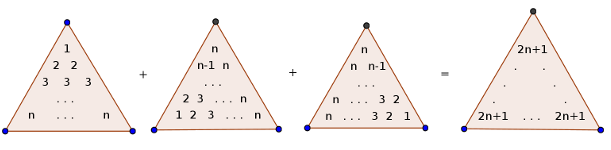
\includegraphics[width=\textwidth]{figure/triangle-proof.png}
\end{minipage}

На языке формул:
\[
  3S = (2n+1) \cdot (1 + 2 + \ldots + n) = (2n+1)n\frac{n+1}{2}.
\]
\end{sol}
\end{problem}




\begin{problem}
  Найдите минимум функции $f(a, b, c) = (6-a)^2 + (3 - b)^2 + (7 - b)^2 + (8 - c)^2 + (9-c)^2 + (10- c)^2 + 11^2$;

  Проекцией какого вектора на какое пространство является вектор $\hat Z = (a, b, b, c, c, c, 0)$?
\begin{sol}
  Проекцией вектора $(6, 3, 7, 8, 9, 10, 11)$; $a=6$, $b=5$, $c= 9$;
\end{sol}
\end{problem}




\begin{problem}
  Вектор $Z$ из $n$ случайных величин имеет многомерное нормальное распределение, $Z_i \sim \cN(0;1)$, и все $Z_i$ независимы.
  Определите, какое распределение имеет величина $Q$, на какое подпространство проецировали вектор $Z$, и найдите вероятность:
  \begin{enumerate}
    \item $Q = Z_1^2$, $\P(Q > 6.6)$;
    \item $Q=n\bar Z^2$, $\P(Q < 3.8)$;
    \item $Q=\sum (Z_i - \bar Z)^2$;
    \item $Q = Z_5^2 + Z_6^2 + Z_{32}^2$, $\P(Q < 0.58)$;
    \item $Q = Z_2^2 + (Z_7 + Z_{11})^2/2$, $\P(Q>6)$;
    \item $Q = (Z_7 + Z_{11})^2/2 + (Z_3 + Z_9 + Z_{12})^2/3$, $\P(Q < 0.21)$;
  \end{enumerate}
  Для каждого случая укажите подпространство, для которого величина $Q$ будет квадратом длины проекции исходного вектора $Z$;
\begin{sol}
\end{sol}
\end{problem}



\begin{problem}
Вектор $Z$ из $n$ случайных величин имеет многомерное нормальное распределение, $Z_i \sim \cN(0;1)$, и все $Z_i$ независимы.
\begin{enumerate}
  \item Какое распределение имеет величина $Q = Z_1^2 + Z_2^2 + \ldots + Z_d^2$?
  \item Чему равно $\E(Q)$?
  \item Чему равна дисперсия $\Var(Q)$?
  \item Величина $Q_a$ имеет хи-квадрат распределение с $a$ степенями свободы, а величина $Q_b$ — с $b$ степенями свободы.
    Величины $Q_a$ и $Q_b$ независимы.
    Какое распределение имеет величина $S=Q_a + Q_b$?
\end{enumerate}

\begin{sol}
\begin{enumerate}
\item $\chi^2_d$
\item $d$
\item $2d$
\item $\chi^2_{a+b}$
\end{enumerate}
\end{sol}
\end{problem}




\begin{problem}
  Найдите функцию плотности $\chi$-квадрат распределения с одной степенью свободы;
\begin{sol}
  $Q= Z_1^2$, зная функцию плотности $Z_1$, $f(z_1) = \frac{1}{\sqrt{2\pi}}\exp(-z_1^2/2)$, находим функцию плотности $Q$;
\end{sol}
\end{problem}



\begin{problem}
Пусть величины $X$ и $Y$ независимы и имеют хи-квадрат распределение с одной степенью свободы. Введём величины $R=X/(X+Y)$ и $S=X+Y$.
\begin{enumerate}
  \item Выпишите совместную функцию плотности $f(x, y)$;
  \item Найдите совместную функцию плотности $f(r, s)$;
  \item Верно ли, что $R$ и $S$ независимы?
  \item С точностью до сомножителя найдите функцию плотности $S$;
  \item Какой закон распределения имеет величина $S$?
\end{enumerate}
\begin{sol}
\end{sol}
\end{problem}


\begin{problem}
Пусть величины $X$ и $Y$ независимы и имеют хи-квадрат распределение с одной и двумя степенями свободы. Введём величины $R=X/(X+Y)$ и $S=X+Y$.
\begin{enumerate}
  \item Выпишите совместную функцию плотности $f(x, y)$;
  \item Найдите совместную функцию плотности $f(r, s)$;
  \item Верно ли, что $R$ и $S$ независимы?
  \item С точностью до сомножителя найдите функцию плотности $S$;
  \item Какой закон распределения имеет величина $S$?
  \item Предположите вид функции плотности хи-квадрат распределения с $d$ степенями свободы и докажите догадку по индукции;
\end{enumerate}
\begin{sol}
\end{sol}
\end{problem}






\begin{problem}
Вектор $Z$ из $n$ случайных величин имеет многомерное нормальное распределение, $Z_i \sim \cN(0;1)$, и все $Z_i$ независимы. Вектор $v$ имеет единичную длину.
\begin{enumerate}
  \item Найдите вектор $\hat Z$, проекцию вектора $Z$ на подпространство $\Lin(v)$; Чему равно $\hat Z_i$?
  \item Найдите дисперсию $\Var(\langle Z, v\rangle)$;
  \item Найдите ковариацию $\Cov(\hat Z_i, \hat Z_j)$;
  \item Как выглядит ковариационная матрица вектора $\hat Z$?
\end{enumerate}

\begin{sol}
  $\hat Z = \langle Z, z\rangle \cdot v$;
$\hat Z_i = \langle Z, z\rangle \cdot v_i$;
$\Var(\langle Z, z\rangle)=1$; $\Cov(\hat Z_i, \hat Z_j)=v_i v_j \Var( \langle Z, z\rangle)= v_i v_j$;
\end{sol}
\end{problem}





\section{Максимально правдоподобно — 1!}


\begin{problem}
 Кот Матроскин каждый вечер ходит на рыбалку. Поймав одну «рыбку» кот Матроскин возвращается домой. В пруду встречаются караси, щуки и бегемоты. Кот Матроскин хочет оценить вероятность $p$ поймать карася. От своей бабушки Кот Матроскин достоверно знает, что щуки встречаются в два раза чаще карасей. За ночь экосистема пруда успевает восстановиться от воздействия кота Матроскина.

\begin{enumerate}
\item Оцените $\hat{p}_{KM}$ методом максимального правдоподобия, если Кот Матроскин ловил «рыбку» четыре дня и имеются наблюдения: $X_1=\text{щука}$, $X_2=\text{карась}$, $X_3=\text{карась}$, $X_4=\text{бегемот}$.
\item Постройте оценку $\hat{p}_{KM}$ методом максимального правдоподобия в общем виде. То есть, Кот Матроскин ходил на пруд $n$ дней, поймал $Y_{\text{к}}$ карасей, $Y_{\text{щ}}$ щук и $Y_{\text{б}}$ бегемотов.
\item Зависимы ли величины $Y_{\text{к}}$, $Y_{\text{щ}}$ и $Y_{\text{б}}$? Как распределена величина $Y_{\text{б}}$? Найдите $\E(Y_{\text{б}})$, $\Var(Y_{\text{б}})$.
\item Найдите $\E(\hat{p}_{\text{KM}})$, $\Var(\hat{p}_{\text{KM}})$
\item Является ли оценка $\hat{p}_{\text{KM}}$ несмещенной, состоятельной?
\item Постройте аналогичную оценку $\hat{p}_{\text{ПШ}}$ для Пса Шарика. В отличие от Кота Матроскина Пёс Шарик не знает, что щуки встречаются в два раза чаще карасей. Является ли оценка Пса Шарика несмещенной и состоятельной?
\item Какая из двух оценок является более эффективной? Почему?
\end{enumerate}

\begin{sol}
  Метод максимального правдоподобия:
  \[
    C_n^{Y_{\text{к}}}C_{n-Y_{\text{к}}}^{Y_{\text{щ}}}a^{Y_{\text{к}}}(2a)^{Y_{\text{щ}}}(1-3a)^{Y_{\text{б}}} \to \max_a
  \]
Решая задачу максимизации Кота Матроскина получаем
\[
\hat a_{КМ} = \frac{Y_{\text{к}} + Y_{\text{щ}}}{3n}
\]

Замечаем, что $Y_{\text{к}} + Y_{\text{щ}} \sim Bin(n, 3a)$. Отсюда $\E(\hat a_{\text{КМ}})=a$, $\Var(\hat a_{\text{КМ}}) = \frac{a(1-3a)}{n}$. Оценка несмещённая и состоятельная.

С точки зрения Пса Шарика, неизвестными являются две вероятности, $a$ и $b$. Он решает задачу максимизации по двум переменным. В результате получается вполне себе интуитивная оценка $\hat a_{\text{ПШ}} = Y_{\text{к}}/n$.

\end{sol}
\end{problem}
\begin{problem}
  «Про зайцев». В темно-синем лесу, где трепещут осины, живут $n >> 0$ зайцев. Мы случайным образом отловили $100$ зайцев. Каждому из них на левое ухо мы завязали бант из красной ленточки и потом всех отпустили. Через неделю будет снова отловлено $100$ зайцев. Из них случайное количество $S$ зайцев окажутся с бантами.

\begin{enumerate}
\item Постройте ML и MM оценку для неизвестного параметра $n$, если оказалось, что $s=80$
\item Постройте ML и MM оценку для неизвестного параметра $n$ в общем случае
\end{enumerate}

\begin{sol}
Метод правдоподобия: $\max_n \P(S=80)$. Замечаем, что $S \sim Bin\left(100, p=\frac{100}{n}\right)$. Отсюда, $\hat n_{ML} = 125$.

Метод моментов. Рассмотрим $Y_1$, $Y_2$, \ldots, $Y_n$. Величина $Y_i$ равна 1 если при втором отлове $i$-ый заяц оказался с бантом и 0 иначе.

Метод моментов: $\E(Y_i)|_{n=\hat n}=\bar Y$:
\[
\frac{100}{\hat n_{MM}}=\bar Y
\]
Отсюда
\[
\hat n_{MM} = \frac{100}{\bar Y} = \frac{100^2}{S}
\]
\end{sol}
\end{problem}
\begin{problem}
 Вася и Петя независимо друг от друга прочитали всю Википедию. Вася всего нашёл 100 опечаток, Петя — 200 опечаток. При этом 80 опечаток оказались найдены и Петей, и Васей. С помощью ML и MM:
\begin{enumerate}
\item Оцените количество опечаток в Википедии
\item Оцените внимательность Васи, то есть вероятность, с которой Вася находит опечатки
\end{enumerate}



\begin{sol}
\end{sol}
\end{problem}
\begin{problem}
  У Васи есть два одинаковых золотых слитка неизвестной массы $m$ каждый и весы, которые взвешивают с некоторой погрешностью. Сначала Вася положил на весы один слиток и получил результат $Y_{1}=m+u_{1}$, где $u_1$ — случайная величина, ошибка первого взвешивания. Затем Вася положил на весы сразу оба слитка и получил результат $Y_{2}=2m+u_{2}$, где $u_2$ — случайная величина, ошибка второго взвешивания. Оказалось, что $y_{1}=0.9$, а $y_{2}=2.3$.


Используя ML оцените вес слитка $m$ и параметр погрешности весов $b$, если
\begin{enumerate}
\item $u_i$ — независимы и $N(0;b)$
\item $u_i$ — независимы и $U[-b;b]$
\end{enumerate}

\begin{sol}
\end{sol}
\end{problem}
\begin{problem}
 Задача о немецких танках
\footnote{Незадолго до высадки союзников в Нормандии, 6 июня 1944 года,
в распоряжении союзников было всего два (!) немецких танка «Пантера V».
По серийным номерам на шасси танков союзники оценили выпуск в феврале 1944 в 270 танков.
Фактический выпуск «Пантер V» согласно немецким документам в феврале 1944 составил 276 танков,
\cite{ruggles1947empirical}.
}

Предположим, что все выпущенные танки имеют порядковый номер.
От самого первого выпущенного танка, имеющего номер $1$, до самого последнего танка, имеющего номер $n$.
В бою удалось подбить танки с номерами $15$, $29$ и $23$.

\begin{enumerate}
\item Постройте оценку количества танков методом моментов
\item Постройте оценку количества танков методом максимального правдоподобия
\item Постройте несмещённую оценку количества танков с наименьшей дисперсией
\end{enumerate}


\begin{sol}
\end{sol}
\end{problem}

\section{Максимально правдоподобно — 2!}



\texttt{Минитеория} \\
Метод моментов (MM, method of moments): найти $\theta$ из уравнения $\bar{X_{n}}=\E(X_{i})|_{\theta=\hat\theta}$ \\
Метод максимального правдоподобия (ML, maximum likelihood): \\
найти $\theta$ при котором вероятность получить имеющиеся наблюдения будет максимальной \\
Наблюдаемая информация Фишера: $\hat{I}=-\frac{\partial^2 l}{\partial^2 \theta}(\hat{\theta})$, $\widehat{\Var}(\hat{\theta}_{ML})=\hat{I}^{-1}$. \\


Пусть $l(\theta)$ — логарифмическая функция правдоподобия ($l(\theta)=\ln(f(X_{1}, \ldots ,X_{n},\theta))$). \\
Ожидаемая информация Фишера $I(\theta)=\E\left[\left(\frac{\partial
l}{\partial \theta}\right)^{2}\right]=-E\left(\frac{\partial^{2}l}{\partial \theta^{2}}\right)$ \\
Сколько информации о неизвестном $\theta$ содержится в выборке $X_{1}$, \ldots , $X_{n}$
%Если $X_{i}$ - независимы и одинаково распределены, то $I(\theta)=n %I_{X_{i}}(\theta)$, где $I_{X_{i}}(\theta)$ - информация о неизвестном $\theta$, %содержащаяся в наблюдении одного $X_{i}$ \\

Неравенство Крамера-Рао (Cramer-Rao) («слишком хорошей оценки не бывает»): \\
Если $\hat{\theta}$ - несмещенная оценка и \ldots , то
$\Var(\hat{\theta})\ge \frac{1}{I(\theta)}$

Оценки ML — самые лучшие (асимптотически несмещенные и с минимальной дисперсий): \\
Если $X_{i}$ — iid, \ldots , и $n\to\infty$ то $\hat{\theta}_{ML}\sim N(\theta,\frac{1}{I(\theta)})$.

%В качестве оценки $\hat{I}$ берут $I(\hat{\theta})$ \\




\begin{problem}
  Допустим, что $X_{i}$ — независимы и имеют закон распределения, заданный табличкой: \\

\begin{tabular}{*{4}{c}}
\toprule
 X & -1 & 0 & 2 \\
\midrule
 $\P()$ & $\theta$ & $2\theta-0.2$ & $1.2-3\theta$ \\
\bottomrule
\end{tabular}


Имеется выборка: $X_{1}=0$, $X_{2}=2$. \\
\begin{enumerate}
\item Найдите оценки $\hat{\theta}_{ML}$ и $\hat{\theta}_{MM}$ \\
\item Первоначально ничего о $\theta$ не было известно и поэтому
предполагалось, что $\theta$ распределена равномерно на
$[0.1;0.4]$. Как выглядит условное распределение $\theta$, если известно что $X_{1}=0$, $X_{2}=2$? \\
\item Постройте ML и MM оценки для произвольной выборки $X_{1}$, $X_{2}$, \ldots $X_{n}$

\end{enumerate}




\begin{sol}
  $\hat{\theta}_{ML}=0.25$, $\hat{\theta}_{MM}=0.2$
  $\hat{\theta}_{MM}=\frac{2{,}4-\bar{X}}{7}$
\end{sol}
\end{problem}
\begin{problem}
  Пусть $Y_{1}$ и $Y_{2}$ независимы и распределены по Пуассону. Известно также, что $\E(Y_{1})=e^{a}$ и $\E(Y_{2})=e^{a+b}$.
\begin{enumerate}
\item Найдите ML оценки $\hat a$ и $\hat b$ для случая $y_1=7$ и $y_2=3$
\item Найдите ML оценки $\hat a$ и $\hat b$ в общем виде
\end{enumerate}


\begin{sol}
$\hat{a}=\ln(Y_{1})$, $\hat{b}=\ln(Y_{2})-\ln(Y_{1})$
\end{sol}
\end{problem}
\begin{problem}
  Пусть  $X_{1}$, \ldots , $X_{n}$  распределены одинаково и независимо.
Оцените значение $\theta $ с помощью ML (везде) и MM (в «а» и «б»), оцените дисперсию ML оценки, если функция плотности $X_{i}$, $p(t)$ имеет вид:
\begin{enumerate}
\item $\theta t^{\theta -1} $  при  $t\in \left[0;1\right]$;
\item $\frac{2t}{\theta ^{2}} $  при  $t\in \left[0;\theta \right]$\\
\item  $\frac{\theta e^{-\frac{\theta ^{2} }{2t} } }{\sqrt{2\pi t^{3}
} } $  при  $t\in \left[0;+\infty \right)$;
\item  $\frac{\theta \left(\ln ^{\theta -1} t\right)}{t} $  при  $t\in
\left[1;e\right]$;
\item   $\frac{e^{-\left|t\right|} }{2\left(1-e^{-\theta } \right)} $
при  $t\in \left[-\theta ;\theta \right]$
\end{enumerate}



\begin{sol}
\end{sol}
\end{problem}
\begin{problem}
  Пусть $X_{1}$, \ldots , $X_{n}$ - независимы и экспоненциальны с параметром $\lambda$. Постройте MM и ML оценки параметра  $\lambda$. Оцените дисперсию ML оценки.

\begin{sol}
\end{sol}
\end{problem}
\begin{problem}
  Пусть $X_{1}$, \ldots , $X_{n}$ - независимы и $N(\mu;\sigma^{2})$. Значение $\sigma^{2}$ известно.  Постройте MM и ML оценки параметра $\mu$.

\begin{sol}
\end{sol}
\end{problem}
\begin{problem}
  Пусть $X_{i}$ независимы и одинаково распределены $N(\alpha,2\alpha)$ \\
По выборке $X_{1}$, \ldots , $X_{n}$ постройте оценку для $\alpha$ с помощью ML и MM. Оцените дисперсию ML оценки.


\begin{sol}
$\hat{a}_{ml}=\sum X_i^2/2n$, $\hat{a}_{mm}=\bar{X}$.
\end{sol}
\end{problem}
\begin{problem}
  Пусть $Y_{1}\sim N(0;\frac{1}{1-\theta^{2}})$. Найдите ML оценку для $\theta$. Оцените дисперсию ML оценки.

\begin{sol}
\end{sol}
\end{problem}
\begin{problem}
  Пусть $X_{1}$, $X_{2}$,\ldots , $X_{n}$ независимы и их функции
плотности имеет вид: \\
$ f(x)=
\left\{%
\begin{array}{ll}
    (k+1)x^{k}, & x \in [0;1]; \\
    0, & x \notin [0;1]. \\
\end{array}%
\right.$ \\
Найдите оценки параметра $k$ с помощью ML и MM. Оцените дисперсию ML оценки.

\begin{sol}
\end{sol}
\end{problem}
\begin{problem}
   Пусть $X_{1}$, $X_{2}$,\ldots , $X_{n}$ независимы и
равномерно
распределены на отрезке $[0;\theta]$, $\theta>1$
\begin{enumerate}
\item Постройте MM и ML оценки для неизвестного $\theta$.
\item Как изменятся ответы на «a», если исследователь не
знает значений самих $X_{i}$, а знает только количество $X_{i}$
оказавшихся больше единицы?
\end{enumerate}



\begin{sol}
\end{sol}
\end{problem}
\begin{problem}
  В озере водятся караси, окуни, щуки и налимы. Вероятности их поймать занесены в табличку \\
\begin{tabular}{*{5}{c}}
\toprule
Рыба: & Карась & Окунь & Щука & Налим \\
\midrule
$\P()$ & 0.1 & $p$ & $p$ & $0.9-2p$ \\
\bottomrule
\end{tabular}

Рыбак поймал 100 рыб и среди пойманных 100 рыб он посчитал количества карасей, окуней, щук и налимов. \\
\begin{enumerate}
\item Постройте $\hat{p}_{ML}$
\item Найдите ожидаемую и наблюдаемую информацию Фишера
\item Несмещенная оценка $\hat{\theta}$ получена по 100
наблюдениям: $X_{1}$, \ldots , $X_{100}$.
В каких пределах может лежать $\Var(\hat{\theta})$?
\end{enumerate}

\begin{sol}
\end{sol}
\end{problem}
\begin{problem}
  Известно, что $X_{i}$ — независимы и имеют закон распределения, заданный таблицей: \\
\begin{tabular}{*{3}{c}}
\toprule
$X_i$ & 0 & 1 \\
\midrule
$\P()$ & $p$ & $1-p$ \\
\bottomrule
\end{tabular}

\begin{enumerate}
\item Постройте $\hat{p}_{ML}$
\item Найдите ожидаемую и наблюдаемую информацию Фишера. Постройте возможные графики $I(p)$.
\item Пусть $\hat{\theta}$ — несмещенная оценка, полученная по 100 наблюдениям: $X_{1}$, \ldots , $X_{100}$. \\
В каких пределах может лежать $\Var(\hat{\theta})$?
\end{enumerate}


\begin{sol}
\end{sol}
\end{problem}
\begin{problem}
  Пусть $X_{i}$ независимы и имеют экспоненциальное распределение с параметром
$\lambda$, т.е. $p(t)=\lambda e^{-\lambda t}$.
\begin{enumerate}
\item Найдите $I(\lambda)$, если наблюдаются $X_{1}$, \ldots , $X_{n}$ \\
\item Пусть $\lambda=1/\theta$, т.е. $p(t)=\frac{1}{\theta}
e^{-\frac{1}{\theta} t}$. Найдите $I(\theta)$, если наблюдается $X_{1}$, \ldots , $X_{n}$
%в) Пусть $\hat{\theta}$ - несмещенная оценка, полученная по 100
%наблюдениям. В каких пределах может лежать $\Var(\hat{\theta})$?
\end{enumerate}





\begin{sol}
\end{sol}
\end{problem}
\begin{problem}
  Пусть $X_{i}$ — независимы и одинаково распределены. Пусть $I_{X_{i}}(\theta)$ - информация Фишера о $\theta$, получаемая при наблюдении $X_{i}$.
\begin{enumerate}
\item  Верно ли, что $I_{X_{1}}(\theta)=I_{X_{2}}(\theta)$?
\item  Как найти $I_{X_{1}, \ldots ,X_{n}}(\theta)$ зная $I_{X_{i}}(\theta)$?
\end{enumerate}


\begin{sol}
\end{sol}
\end{problem}


\begin{problem}
  Величины $X_{1}$, \ldots , $X_{n}$ — независимы и одинаково распределены с функцией плотности $f(t)=\frac{\theta \left(\ln  t\right)^{\theta -1}}{t} $  при  $t\in
\left[1;e\right]$. По выборке из 100 наблюдений оказалось, что $\sum{\ln(\ln(X_{i}))}=-30$
\begin{enumerate}
\item Найдите ML оценку параметра $\theta$ и ожидаемую и наблюдаемую информацию Фишера
\item Постройте 95\% доверительный интервал для $\theta$
\end{enumerate}


\begin{sol}
\end{sol}
\end{problem}
\begin{problem}
  Величины $X_{1}$, \ldots , $X_{n}$ — независимы и одинаково распределены с функцией плотности $\frac{\theta e^{-\frac{\theta^{2}}{2t}}}{\sqrt{2\pi t^{3}
}}$ при $t\in \left[0;+\infty \right)$. По выборке из 100 наблюдений оказалось, что $\sum{1/X_{i}}=12$
\begin{enumerate}

\item Найдите ML оценку параметра $\theta$ и информацию Фишера $I(\theta)$
\item  Пользуясь данными по выборке постройте оценку $\hat{I}$ для информации Фишера
\item  Постройте 90\% доверительный интервал для $\theta$
Hint: $\E(1/X_{i})=1/\theta^{2}$ (интеграл берется заменой $x=\theta^{2}a^{-2}$)
\end{enumerate}

\begin{sol}
\end{sol}
\end{problem}



\begin{problem}
  Известно, что $X_i$ независимы, $\E(X_i)=5$, $\Var(X_i)=4$ и $n$ велико. Как примерно распределены следующие величины:
\begin{enumerate}
\item $\bar{X}_n$,
\item $Y_n=(\bar{X}_n+3)/(\bar{X}_n+6)$,
\item $Z_n=\bar{X}_n^2$,
\item $W_n=1/\bar{X}_n$
\end{enumerate}

\begin{sol}
\end{sol}
\end{problem}
\begin{problem}
  Известно, что $X_i$ независимы и равномерны на $[0;1]$.
\begin{enumerate}

\item  Найдите $\E(\ln(X_i))$, $\Var(\ln(X_i))$, $\E(X_i^2)$, $\Var(X_i^2)$

\item Как примерно распределены величины $X_n=\frac{\sum\ln(X_i)}{n}$, $Y_n=(X_1\cdot X_2\cdots X_n)^{1/n}$, $Z_n=\left(\frac{\sum X_i^2}{n} \right)^3$ при больших $n$?
\end{enumerate}

\begin{sol}
\end{sol}
\end{problem}
\begin{problem}
  Величины $X_i$ независимы и имеют функцию плотности $f(x)=a\cdot x^{a-1}$ на отрезке $[0;1]$.

\begin{enumerate}
\item Постройте оценку $\hat{a}$ методом моментов, укажите её примерный закон распределения

\item По 100 наблюдениям оказалось, что $\sum X_i=25$. Посчитайте численное значение $\hat{a}$ и оцените дисперсию случайной величины $\hat{a}$.
\end{enumerate}

\begin{sol}
\end{sol}
\end{problem}
\begin{problem}
 Начинающий каратист Вася тренируется бить кирпичи ударом ладони. Каждый день он бьёт ладонью по кирпичу до пор, пока тот не расколется от одного удара. Предположим, что вероятность разбить кирпич с одного удара равна $p$ и неизменна во времени. Величины $X_1$, $X_2$, \ldots, $X_n$ — количества ударов которые потребовались Васе в соответствующий день.

\begin{enumerate}
\item Найдите оценку $p$ методом максимального правдоподобия
\item Найдите достаточную статистику $T$
\item Выразите $\hVar(\hat{p})$ через достаточную статистику $T$
\item Найдите $\P(X_1=1 \mid T=t)$.
\end{enumerate}

\begin{sol}
\end{sol}
\end{problem}
\begin{problem}
 Продавщица Глафира отдаёт псу Шарику в конце каждого дня нерасфасованные остатки мясного фарша. Фарш фасуется упаковками по $a$ грамм, поэтому нерасфасованный остаток в $i$-ый день, $X_i$, случаен и равномерно распределен на отрезке $[0;a]$. Пёс Шарик хорошо помнит все $X_1$, \ldots, $X_n$. Помогите псу Шарику:

\begin{enumerate}
\item Найдите оценку $a$ методом максимального правдоподобия
\item Найдите достаточную статистику $T$
\item Выразите $\hVar(\hat{a})$ через достаточную статистику $T$
\item Найдите $\P(X_1<10 \mid T=t)$.
\end{enumerate}

\begin{sol}
\end{sol}
\end{problem}
\begin{problem}
 Величины $X_i$ равномерны на отрезке $[-a; 3a]$ и независимы. Есть несколько наблюдений, $X_1=0.5$, $X_2=0.7$, $X_3=-0.1$.

\begin{enumerate}
\item Найдите $\E(X_i)$ и $\E(|X_i|)$
\item Постройте оценку метода моментов, используя $\E(X_i)$
\item Постройте оценку метода моментов, используя $\E(|X_i|)$
\item Постройте оценку обобщёного метода моментов используя моменты $\E(X_i)$, $\E(|X_i|)$ и взвешивающую матрицу
\[
W=\begin{pmatrix}
2 & 0 \\
0 & 1 \\
\end{pmatrix}
\]
\item Найдите оптимальную теоретическую взвешивающую матрицу для обобщённого метода моментов
\item Постройте двухшаговую оценку обобщённого метода моментов, начав со взвешивающей матрицы $W$

\end{enumerate}


\begin{sol}
\begin{enumerate}
\item $\E(X_i) = a$, $\E(|X_i|) = 5a/4$
\item $\hat a = 11/30$
\item $\hat a = 26/75$
\item $\hat{a}_{GMM} = 108/325$
\item $\begin{pmatrix}
37 & -44 \\
-44 & 64
\end{pmatrix}$
\end{enumerate}
\end{sol}
\end{problem}
\begin{problem}
 Величины $X_i$ имеют Пуассоновское распределение с параметром $\lambda$ и независимы. Есть несколько наблюдений, $X_1=5$, $X_2=7$, $X_3=1$.

\begin{enumerate}
\item Найдите $\E(X_i)$ и $\E((X_i-\bar X)^2)$
\item Постройте оценку метода моментов, используя $\E(X_i)$
\item Постройте оценку метода моментов, используя $\E((X_i-\bar X)^2)$
\item Постройте оценку обобщёного метода моментов используя моменты $\E(X_i)$, $\E((X_i-\bar X)^2)$ и взвешивающую матрицу
\[
W=\begin{pmatrix}
3 & 0 \\
0 & 1 \\
\end{pmatrix}
\]
\item Найдите оптимальную теоретическую взвешивающую матрицу для обобщённого метода моментов
\item Постройте двухшаговую оценку обобщённого метода моментов, начав со взвешивающей матрицы $W$

\end{enumerate}


\begin{sol}
\end{sol}
\end{problem}


\begin{problem}

Величины $X_1$, \ldots, $X_n$ независимы и равномерны на отрезке $[-1; 1]$. Величины $Y_1$, \ldots, $Y_n$ независимы и имеют на отрезке $[-1; 1]$ функцию плотности

\[
h(y) = \frac{3\exp(\alpha^{-4})}{4}(1 - \exp(2\alpha^{-4})(y+\alpha - 1)^2)
\]

Исследовательница Зинаида создаёт величины $Z_1$, \ldots, $Z_n$ по простому принципу. Каждая $Z_i$ равна $Y_i$ с вероятностью $\alpha$ и $X_i$ с вероятностью $(1-\alpha)$.

Пусть $n=500$.

\begin{enumerate}
\item Постройте выборку из $X_i$ и изобразите результат с помощью гистограммы.
\item Постройте выборку из $Y_i$ при $\alpha = 0.5$ и изобразите результат на гистограмме.
\item Постройте выборку из $Z_i$ при $\alpha = 0.5$ и изобразите результат на гистограмме.
\end{enumerate}

У рассеянной Зинаиды сохранилась только выборка из $Z_i$. Она не помнит ни $\alpha$, ни $X_i$, ни $Y_i$. И поэтому Зинаида решила восстановить $\alpha$ с помощью максимального правдоподобия.

\begin{enumerate}[resume]

\item Для полученной выборки $Z_i$ постройте график функции правдоподобия. Будьте осторожны! Если по-быстрому строить график командой встроенной в R/python/julia/\ldots, то получится неверный график! Обратите внимание на значения функции в точках $Z_i$.

\item Найдите оценку максимального правдоподобия для параметра $\alpha$ по полученной выборке.

\item Найдите $\plim_{n\to\infty} \hat\alpha_{ML}(n)$ для произвольного $\alpha$. Является ли оценка $\hat\alpha_{ML}$ состоятельной?

\end{enumerate}

\begin{sol}
  $\plim_{n\to\infty} \hat\alpha_{ML}(n) = 0$, не является состоятельной
\end{sol}
\end{problem}


\begin{problem}
Величины $X_1$, \ldots, $X_n$ независимы и одинаково распределены с функцией распределения
\[
	F(x)=1/(1+\exp(a-x))
\]

Рассмотрим три оценки: оценку максимального правдоподобия, $\hat a_{ML}$, простую медиану $\hat a_{Med} = \Med{X_1, \ldots, X_n}$ и скорректированную медиану $\hat a_{1step}=\hat a_{Med} - \frac{\ell'(\hat a_{Med})}{\ell''(\hat a_{Med})}$.

\begin{enumerate}
  \item Существует ли в явном виде формула для $\hat a_{ML}$ в этой задаче?
  \item Сгенерируйте 1000 выборок по $n=20$ наблюдений в каждой для $a=2$. Для каждой выборки найдите оценки трёх видов. Таким образом получится 1000 оценок каждого вида. Рассчитайте выборочную дисперсию и выборочное среднее каждой оценки.
\item Прокомментируйте полученные результаты
\end{enumerate}



\begin{sol}

\end{sol}
\end{problem}


\section{Настоящий ценитель}

\begin{problem}
Случайные величины $X_1$, $X_2$, \ldots независимы и одинаково распределены с неизвестными $\E(X_i)=\mu$ и $\Var(X_i)=\sigma^2$. Исследовательница Борислава хочет использовать оценку вида $\hat\mu = c (X_1 + X_2 + \ldots + X_n)$ для неизвестного параметра $\mu$.
\begin{enumerate}
  \item При каком $c$ оценка Бориславы будет несмещённой? Возможно ли использовать такое $c$ в практической задаче?
  \item При каком $c$ будет минимальной величина $MSE = \E((\hat \mu -\mu)^2)$? Возможно ли использовать такое $c$ в практической задаче?
  \item Святозар минимизирует по $\hat\mu$ штрафную функцию
  \[
  Q(\hat\mu) = \sum (y_i - \hat\mu)^2 + \lambda \hat\mu^2.
  \]
  При каком $\lambda$ оценка Святозара совпадёт с несмещённой оценкой Бориславы? С оценкой минимизирующей MSE?
\end{enumerate}
  \begin{sol}
    \begin{enumerate}
      \item $c=1/n$, да
      \item $c=1/(n+\sigma^2/\mu^2)$, нет, так как $\mu$ и $\sigma$ неизвестны
      \item $\lambda=0$ и $\lambda=\sigma^2/\mu^2$
    \end{enumerate}
  \end{sol}
\end{problem}

\begin{problem}
Исследовательница Радомира размышляет о том, как оценить неизвестное математическое ожидание по выборке из независимых одинаково распределённых случайных величин. Она мучительно выбирает из нескольких оценок. Для каждой оценки определите, является ли она несмещённой, состоятельной и линейной по наблюдениям. Для линейных несмещённых оценок определите, являются ли они эффективными среди линейных несмещённых оценок.
\begin{enumerate}
\item Удалить из выборки наблюдение номер 13 и посчитать среднее арифметическое.
\item Удалить из выборки все нечётные наблюдения и посчитать среднее арифметическое.
\item Удалить из выборки все наблюдения после 13-го и посчитать среднее арифметическое.
\item Домножить наблюдение номер 13 на 13 и посчитать среднее арифметическое.
\item Прибавить число 13 к наблюдению номер 13 и посчитать среднее арифметическое.
\item Продублировать 13-ое наблюдение 13 раз и посчитать среднее арифметическое.
\item Продублировать каждое наблюдение 13 раз и посчитать среднее арифметическое.
\item Домножить первое наблюдения на 1, второе — на 2, третье — на 3, и так далее и посчитать среднее арифметическое.
\item Прибавить к первому наблюдению 1, ко второму — 2, к третьему — 3, и так далее и посчитать среднее арифметическое.
\item Продублировать первое наблюдения 1 раз, второе — 2 раза, третье — 3 раза, и так далее и посчитать среднее арифметическое.
\end{enumerate}
  \begin{sol}
    \begin{enumerate}
    \item несмещённая, состоятельная, линейная, неэффективная
    \item несмещённая, состоятельная, линейная, неэффективная
    \item несмещённая, несостоятельная, линейная, неэффективная
    \item смещённая, состоятельная, линейная
    \item смещённая, состоятельная, нелинейная
    \item несмещённая, состоятельная, линейная, неэффективная
    \item несмещённая, состоятельная, линейная, эффективная
    \item смещённая, несостоятельная, линейная
    \item смещённая, несостоятельная, нелинейная
    \item несмещённая, состоятельная, линейная, неэффективная
    \end{enumerate}
  \end{sol}
\end{problem}

\begin{problem}
Величины $Y_i$ независимы и имеют функцию плотности
\[
f(y) = \begin{cases}
5y^4/\theta^5, \text{ если } y\in[0;\theta]; \\
0, \text{ иначе.}
\end{cases}
\]

\begin{enumerate}
\item Найдите ML оценку неизвестного параметра $\theta$.
\item Устно, не производя вычислений, определите, является ли оценка $\hat\theta = \max\{ Y_1, Y_2, \ldots, Y_n\}$ несмещённой.
\item Найдите функцию распределения $Y_1$, функцию распределения $\hat\theta$, функцию плотности $\hat\theta$.
\item Найдите $\E(\hat\theta)$.
\item Если $\hat\theta$ смещённая, то скорректируйте оценку так, чтобы она стала несмещённой.
\end{enumerate}


\begin{sol}
\begin{enumerate}
\item $\hat\theta_{ML} = \max\{ Y_1, Y_2, \ldots, Y_n\}$.
\item Все $Y_i$ меньше $\theta$, значит и $\hat\theta$ всегда меньше $\theta$, значит смещённая.
\item $F_{\hat\theta}(t) = \P(\hat\theta \leq t) = \P(Y_1 \leq t, Y_2 \leq t, \ldots) = (\P(Y_1 \leq t))^n$, $\P(Y_1 \leq t) = t^5/\theta^5$, $f_{\hat\theta}(t) = dF_{\hat\theta}(t)/dt = \frac{5n t^{5n-1}}{\theta^{5n}}$.
\item $\E(\hat\theta) = \frac{5n}{5n+1}\theta$.
\item $\hat\theta_{unbiased} = \frac{5n+1}{5n}\hat\theta$.
\end{enumerate}
\end{sol}
\end{problem}


\begin{problem}
Величина $Y$ имеет биномиальное распределение $Bin(n, p)$.
\begin{enumerate}
\item Является ли оценка $\hat p = Y/n$ для $p$ несмещённой? Если является смещённой, то скорректируйте оценку так, чтобы она стала несмещённой.
\item Чему равна теоретическая дисперсия $\sigma^2$ величины $Y$?
\item Является ли оценка $\hat \sigma^2 = n \hat p (1- \hat p)$ для $\sigma^2$ несмещённой? Если является смещённой, то скорректируйте оценку так, чтобы она стала несмещённой.
\end{enumerate}

\begin{sol}
\begin{enumerate}
  \item $\hat p$ несмещённая
  \item $\sigma^2 = n p(1-p)$.
  \item $\E(\hat\sigma^2) = (n-1)p(1-p)$, смещённая, $\hat\sigma^2_{unbiased} = \frac{n}{n-1} \hat\sigma^2$.
\end{enumerate}
\end{sol}
\end{problem}


\begin{problem}
Величины $X_{i}$ независимы и одинаково распределениы. Какая из приведенных оценок для
$\mu=\E\left(X_{i} \right)$  является несмещенной? Обладает наименьшей дисперсией среди несмещённых оценок? Обладает наименьшей среднеквадратичной ошибкой $MSE$?
\begin{enumerate}
\item $X_{1} +3X_{2} -2X_{3} $ ;
\item ${\left(X_{1}
+X_{2} \right)\mathord{\left/ {\vphantom {\left(X_{1} +X_{2}
\right) 2}} \right. \kern-\nulldelimiterspace} 2} $ ;
\item  ${\left(X_{1} +X_{2} +X_{3} \right)\mathord{\left/ {\vphantom
{\left(X_{1} +X_{2} +X_{3} \right) 3}} \right.
\kern-\nulldelimiterspace} 3} $ ;
\item $\left(X_{1} +\ldots +X_{20} \right)/21$ ;
\item $X_{1} -2X_{2} $.
\end{enumerate}
\begin{sol}

\end{sol}
\end{problem}

\begin{problem}
Величина  $X$  равномерна на  $\left[0;a\right]$ . Придумайте несмещённую оценку параметра $a$ вида
$\hat{a}=\alpha +\beta X$.
\begin{sol}

\end{sol}
\end{problem}

\begin{problem}
Величины  $X_{i} $  - независимы и одинаково распределены. При
каком значении параметра  $\beta $

\begin{enumerate}
\item оценка $2X_{1} -5X_{2} +\beta X_{3} $  будет несмещённой  для $\E\left(X_{i} \right)$ ?
\item оценка $\beta \left(X_{1} +X_{2} -2X_{3} \right)^{2} $  будет несмещённойдля  $\Var\left(X_{i} \right)$ ?
\end{enumerate}
\begin{sol}

\end{sol}
\end{problem}

\begin{problem}
Величины  $X_{1} $  и  $X_{2} $  независимы и равномерны на
$\left[0;a\right]$ . При каком  $\beta $  оценка  $Y=\beta \cdot \min \left\{X_{1} ,X_{2} \right\}$  для параметра  $a$  будет
несмещённой?
\begin{sol}

\end{sol}
\end{problem}

\begin{problem}
Величины $X_{i}$ независимы и одинаково распределены. Какая из приведенных оценок для
$\sigma^2 = \Var\left(X_{i} \right)$  является несмещённой?

\begin{enumerate}
\item  $X_{1}^{2} -X_{1} X_{2} $ ;
\item  $\frac{\sum_{i=1}^{n}\left(X_{i} -\bar{X}\right)^{2}  }{n} $ ;
\item $\frac{\sum _{i=1}^{n}\left(X_{i} -\bar{X}\right)^{2}  }{n-1} $ ;
\item  $\frac{1}{2} \left(X_{1} -X_{2} \right)^{2} $ ;
\item  $X_{1} -2X_{2} $ ;
\item $X_{1} X_{2} $.
\end{enumerate}
\begin{sol}

\end{sol}
\end{problem}

\begin{problem}
Величина $X$  равномерна на  $\left[3a-2;3a+7\right]$ . При
каких  $\alpha $  и  $\beta $  оценка  $Y=\alpha +\beta X$
неизвестного параметра  $a$  будет несмещённой?
\begin{sol}

\end{sol}
\end{problem}

\begin{problem}
Закон распределения величины  $X$  имеет вид

\begin{enumerate}
\item  $\begin{array}{|c|ccc|}  \hline {x_{i} } & {0} & {1} & {a} \\
\hline {P\left(X=x_{i} \right)} & {{1\mathord{\left/ {\vphantom {1
4}} \right. \kern-\nulldelimiterspace} 4} } & {{1\mathord{\left/
{\vphantom {1 4}} \right. \kern-\nulldelimiterspace} 4} } &
{{2\mathord{\left/ {\vphantom {2 4}} \right.
\kern-\nulldelimiterspace} 4} } \\  \hline  \end{array}$ ;
\item $\begin{array}{|c|ccc|}  \hline {x_{i} } & {0} & {1} & {2} \\
\hline {P\left(X=x_{i} \right)} & {{1\mathord{\left/ {\vphantom {1
4}} \right. \kern-\nulldelimiterspace} 4} } & {a} &
{\left({3\mathord{\left/ {\vphantom {3 4}} \right.
\kern-\nulldelimiterspace} 4} -a\right)} \\  \hline  \end{array}$
\end{enumerate}

Постройте несмещённую оценку вида  $Y=\alpha +\beta X$  для
неизвестного параметра  $a$.
\begin{sol}

\end{sol}
\end{problem}

\begin{problem}
Время горения лампочки распределено экспоненциально с
ожиданием равным  $\theta$ . Вася включил одновременно 20
лампочек. Величина $X$  обозначает время самого первого перегорания. Как с помощью $X$  построить несмещенную оценку для  $\theta $ ?
\begin{sol}
  Закон распределения $X$ также экспоненциальный, но с другим $\lambda$. Честно находим $\E(X)=\theta/20$, отсюда
  $\hat\theta_{unbiased} = 20X$.
\end{sol}
\end{problem}

\begin{problem}
Величины $X_{i}$ независимы и одинаково распределены, причем
$\Var(X_{i})=\sigma^{2}$, а $\E(X_{i})=\frac{\theta}{\theta+1}$, где
$\theta>0$ — неизвестный параметр. С помощью $\bar{X}$ постройте состоятельную оценку для $\theta$.
\begin{sol}

\end{sol}
\end{problem}

\begin{problem}
Величины $Y_{i}=\beta x_{i} +\varepsilon_{i}$, константа $\beta$ и
случайные величины $\varepsilon_{i}$ являются ненаблюдаемыми.
Известно, что $\E(\epsilon_{i})=0$, $\Var(\epsilon_{i})=1$,
$\epsilon_{i}$ являются независимыми. Константы $x_{i}$
наблюдаемы, и известно, что $20<x_{i}<100$. У исследователя есть
две
оценки для $\beta$: $\hat{\beta}_{1}=\frac{\bar{Y}}{\bar{x}}$ и
$\hat{\beta}_{2}=\frac{\sum{x_{i}Y_{i}}}{\sum x_{i}^{2}}$.

\begin{enumerate}
\item Проверьте несмещенность, состоятельность.
\item Определите, какая оценка из двух является наиболее эффективной.
\end{enumerate}
\begin{sol}
Обе оценки несмещённые, состоятельные. Более эффективна $\hat{\beta}_{2}=\frac{\sum{x_{i}Y_{i}}}{\sum x_{i}^{2}}$.
\end{sol}
\end{problem}


\begin{problem}
Исследователи Иван да Марья интересуются, какая доля населения берёт взятки. Они независимо друг от друга задают разным людям вопрос: «Берёте ли Вы взятки?»

Иван использует следующий механизм: предлагает респонденту тайно подбросить правильную монетку, если монетка выпадает орлом, то предлагается ответить «да», если решкой — то предлагается ответить правду. Предположим, что все респонденты действую точно так, как предлагает Иван.

У Марьи кристально чистые голубые глаза, она юна и невинна, и солгать ей просто невозможно.

Пусть $p$ — доля берущих взятки, а $\hat q_{I}$ и $\hat q_{M}$ — доля ответивших «да» на вопросы Ивана да Марьи. Марья использует оценку $\hat p_M = \hat q_M$, а Иван — $\hat p_I = 2\hat q_I - 1$.

\begin{enumerate}
\item Являются ли оценки $\hat p_M$, $\hat p_I$ несмещёнными? состоятельными?
\item Иван планирует опросить 100 человек. Сколько человек в завимости от $p$ нужно опросить Марье, чтобы $\Var(\hat p_I) = \Var(\hat p_M)$?
\end{enumerate}

Идея: Кирилл Фурманов
\begin{sol}

\end{sol}
\end{problem}


\section{Классические интервальные оценки}

Здесь интервальные оценки без гипотез :)


\begin{problem}
  Пусть $X$ — равномерна на участке $[0;2a]$. С какой вероятностью интервал $[0.9X;1.1X]$ накрывает неизвестное $a$? Постройте 95\%-ый доверительный интервал для $a$ вида $[0;kX]$.
\begin{sol}
 Переформулируем задачу следующим образом: $\P(0.9X\leq a \leq1.1X)=\P(\frac{10}{11}a\leq X \leq \frac{10}{9}a)=\frac{\frac{10}{9}a-\frac{10}{11}a}{2a}=\frac{10}{99}$. Поскольку $a$ неотрицательно по условию, $\P(a\in[0;kX])=\P(a\leq kX)$. Найдём такое $k$, что последняя вероятность равна 0.95: $$1-\P\left(X\leq\frac{a}{k}\right)=0.95$$
  $$1-\frac{\frac{a}{k}}{2a}=0.95$$
  $$k=10$$
\end{sol}
\end{problem}

\begin{problem}
  Пусть $X$ — экспоненциальна с параметром $\lambda$ и $\mu=\E(X)$. C какой вероятностью интервал $[0.9X;1.1X]$ накрывает $\mu$? Постройте 90\%-ый доверительный интервал для $\mu$ вида $[0;kX]$.
\begin{sol}
%Переформулируем задачу следующим образом: \multline{$$\P(0.9X\leq %\mu \leq1.1X)=\P\left(\frac{10}{11}\mu\leq X \leq %\frac{10}{9}\mu\right)=\\=\int^{\frac{10}{9}\mu}_{\frac{10}{11}\mu}%\lambda{e^{-\lambda x} \, %dx}=[\mu=\lambda^{-1}]=e^{-\frac{10}{11}}-e^{-\frac{10}{9}}.$$\\}
%Поскольку $\mu$ неотрицательно по условию, %$\P(\mu\in[0;kX])=\P(\mu\leq kX)$. Найдём такое $k$, что последняя %вероятность равна 0.9: $$1-\P\left(X\leq\frac{\mu}{k}\right)=0.9$$
%$$1-1+e^{\frac{-\lambda}{k\lambda}}=0.9$$
%$$k=-\frac{1}{\ln{0.9}}.$$
\end{sol}
\end{problem}

\begin{problem}
  Пусть $X_i$ — независимы и нормальны $N(\mu,1)$. Какова вероятность того, что интервал $[\bar{X}_{10}-1;\bar{X}_{10}+1]$ накроет неизвестное $\mu$? Постройте 90\%-ый доверительный интервал для $\mu$ вида $[\bar{X}_{10}-k;\bar{X}_{10}+k]$.
\begin{sol}
Переформулируем задачу следующим образом:$$ \P(\bar{X}_{10}-1\leq \mu \leq\bar{X}_{10}+1)=\P(\mu-1\leq\bar{X}_{10}\leq\mu+1)=$$$$=\P\left(-\sqrt{10}\leq\frac{\bar{X}_{10}-\mu}{\sqrt{\frac{1}{10}}}\leq\sqrt{10}\right)$$
Вспомним, что $\bar{X}_{10} \sim \cN(\mu;\frac{1}{10})$, а значит,  $$\P\left(-\sqrt{10}\leq\frac{\bar{X}_{10}-\mu}{\sqrt{\frac{1}{10}}}\leq\sqrt{10}\right)\approx0.9984.$$ Построим 90\%-й доверительный интервал (симметричность обеспечена свойствами нормального распределения):$$-1.55\leq\frac{\bar{X}_{10}-\mu}{\sqrt{\frac{1}{10}}}\leq1.55$$$$-0.5+\bar{X}_{10}\leq\mu\leq0.5+\bar{X}_{10}.$$

\end{sol}
\end{problem}


\begin{problem}
Вася наугад поймал 400 покемонов-девочек и 100 покемонов-мальчиков. Среди девочек 250 оказались ядовитыми, среди мальчиков — 60.
\begin{enumerate}
 \item Найдите точечную оценку $\hat p$ для доли ядовитых покемонов среди мальчиков.
 \item Найдите точечную оценку $\hat \sigma^2$ для дисперсии $X_i$, где $X_i$ — индикатор ядовитости $i$-го покемона-мальчика.
 \item Постройте 95\%-ый доверительный интервал для доли ядовитых покемонов среди мальчиков.
 \item Постройте 95\%-ый доверительный интервал для доли ядовитых покемонов среди девочек.
 \item Постройте 95\%-ый доверительный интервал для разницы долей ядовитых покемонов среди девочек и мальчиков.
 \item Нужно ли предположение о нормальности $X_i$ и $Y_i$ для решения предыдущих пунктов?
\end{enumerate}
\begin{sol}
\end{sol}
\end{problem}

\begin{problem}
Вася наугад поймал 400 покемонов-девочек и 100 покемонов-мальчиков. Средний рост покемонов-девочек равен $0.9$ метра, и сумма квадратов ростов равна $\sum Y_i^2 =1000$. Для покемонов мальчиков средний рост равен $1$ метру, а сумма квадратов ростов равна $\sum X_i^2 =2000$.
\begin{enumerate}
 \item Постройте точечную оценку для ожидания роста покемона-мальчика $\mu_X$.
 \item Постройте точечную оценку для дисперсии роста покемона-мальчика $\sigma^2_X$.
 \item Постройте 95\%-ый доверительный интервал для ожидаемого роста покемона-мальчика.
\item Постройте 95\%-ый доверительный интервал для ожидаемого роста покемона-девочки.
\item Постройте 95\%-ый доверительный интервал для разницы ожидаемых ростов покемона-мальчика и покемона-девочки.
\item Нужно ли предположение о нормальности $X_i$ и $Y_i$ для решения предыдущих пунктов?
\end{enumerate}
\begin{sol}
\end{sol}
\end{problem}


\begin{problem}
  В одном тропическом лесу длина удавов имеет нормальное распределение $\cN(\mu, \sigma^2)$. По выборке из 10 удавов оказалось, что $\sum Y_i = 20$ метрам, а $\sum Y_i^2 = 1000$.
\begin{enumerate}
  \item Постройте 95\%-ый доверительный интервал для $\mu$.
  \item Постройте 95\%-ый доверительный интервал для $\sigma^2$.
  \item Важна ли предпосылка о нормальности при решении предыдущих пунктов?
\end{enumerate}

\begin{sol}
Важна при обоих доверительных интервалах. Без предпосылки о нормальности интервал для дисперсии по данным формулам нельзя построить даже при больших $n$. При больших $n$ можно отказаться от предпосылки о нормальности при построении интервала для $\mu$.
\end{sol}
\end{problem}


\begin{problem}
  В одном тропическом лесу водятся удавы и питоны. Длина удавов имеет нормальное распределение $\cN(\mu_X, \sigma^2_X)$. По выборке из 10 удавов оказалось, что $\sum X_i = 20$ метрам, а $\sum X_i^2 = 1000$. Длина питонов имеет нормальное распределение $\cN(\mu_Y, \sigma^2_Y)$. По выборке из 20 питонов оказалось, что $\sum Y_i = 60$ метрам, а $\sum Y_i^2 = 4000$.
\begin{enumerate}
  \item Постройте точечные оценки для $\mu_X$, $\sigma^2_X$, $\mu_Y$, $\sigma^2_Y$.
  \item Постройте 95\%-ый доверительный интервал для $\sigma^2_X/\sigma^2_Y$.
  \item Постройте 95\%-ый доверительный интервал для разницы  $\mu_X - \mu_Y$ предполагая равенство дисперсий $\sigma^2_X = \sigma^2_Y$.
  \item Важна ли предпосылка о нормальности при решении предыдущих пунктов?
\end{enumerate}
\begin{sol}
\end{sol}
\end{problem}

\section{Проверка гипотез: общая теория}


\begin{problem}
 Кальямпуди Радхакришна Рао и Карл Харальд Крамер строят доверительный интервал для $\mu$ по случайной выборке из $n$ наблюдений.
Наблюдения, величины $X_i$, распределены нормально и независимы друг от друга.
Рао знает величину $\sigma^2$; а Крамер не знает, и поэтому вынужден использовать $\hat\sigma^2$ при проверке гипотезы.
\begin{enumerate}
\item Какова вероятность того, что Рао получит более короткий доверительный интервал при $n=10$?
\item К чему стремится эта вероятность при $n \to \infty$?

\end{enumerate}
\begin{sol}
к 1/2
\end{sol}
\end{problem}


\begin{problem}
 Как распределено P-значение при верной $H_0$? Вовочка использует следующий статистический критерий: «Если P-значение больше 0.95, то $H_0$ отвергается». Чему де-факто равна вероятность ошибки первого рода в этом случае? Разумно ли использовать данный критерий?


\begin{sol}
  равномерно, $\alpha=0.05$; нет, он резко увеличивает ошибку второго рода
\end{sol}
\end{problem}


\begin{problem}
Величины $X_1$ и $X_2$ независимы и равномерны на отрезке $[0;a]$. Есть две гипотезы, $H_0$: $a=1$ и $H_a$: $a=2$. Мальвина отвергает $H_0$ в том случае, если $X_1 + X_2 > 1.5$. Найдите вероятность ошибок первого и второго рода.
\begin{sol}
  Равномерность обеих случайных величин на $[0;a]$ означает, что пару $(X_1,X_2)$ можно считать координатами точки, выбранной наугад в квадрате со стороной $a$. Пусть верна $H_0$, т.е. сторона квадрата равна 1. Но $H_0$ отвергается, если $X_1+X_2>1.5$ (выбрана точка выше прямой $X_1+X_2=1.5$), поэтому вероятность совершить ошибку первого рода равна вероятности попасть в закрашенную область на первом рисунке ниже (отношению её площади к площади всего квадрата): $\P(\mbox{ошибка 1-го рода})=\frac{1}{2}\cdot\frac{1}{2}\cdot\frac{1}{2}=\frac{1}{8}.$

\begin{figure}[!h]
\begin{center}
\begin{tikzpicture}


\draw[->] (0,0) -- (2,0) coordinate (x axis) 
node [anchor=west]
{$X_1$};
\draw[->] (0,0) -- (0,2) coordinate (y axis) 
node [anchor=south]
{$X_2$};
\draw(0,0) -- (2,0);
\foreach \y in {0.5,1,1.5}
\draw (1pt,\y cm) -- (-1pt,\y cm)
node[anchor=east] {$\y$};
\draw(0,0) -- (0,2);
\foreach \x in {0,0.5,1,1.5}
\draw (\x cm,1pt) -- (\x cm,-1pt)
node[anchor=north] {$\x$};
\draw(0,0) rectangle (1,1);
\draw(0,1.5) -- (1.5,0);
\fill[blue!20!white](1,1) -- (0.5,1) -- (1,0.5);

\end{tikzpicture}
\end{center}
\end{figure}


Пусть верна $H_a$, т.е. сторона квадрата равна 2. Аналогично, ошибка второго рода будет допущена, если выбрана точка ниже прямой $X_1+X_2=1.5$ (см. второй рисунок ниже). $\P(\mbox{ошибка 2-го рода})=\frac{\frac{1}{2}\cdot\frac{3}{2}\cdot\frac{3}{2}}{4}=\frac{9}{32}.$

\begin{figure}[!h]
\begin{center}
\begin{tikzpicture}


\draw[->] (0,0) -- (3,0) coordinate (x axis) 
node [anchor=west]
{$X_1$};
\draw[->] (0,0) -- (0,3) coordinate (y axis) 
node [anchor=south]
{$X_2$};
\draw(0,0) -- (2,0);
\foreach \y in {0.5,1,1.5,2}
\draw (1pt,\y cm) -- (-1pt,\y cm)
node[anchor=east] {$\y$};
\draw(0,0) -- (0,2);
\foreach \x in {0,0.5,1,1.5,2}
\draw (\x cm,1pt) -- (\x cm,-1pt)
node[anchor=north] {$\x$};
\draw(0,0) rectangle (2,2);
\draw(0,1.5) -- (1.5,0);
\fill[blue!20!white](0,0) -- (1.5,0) -- (0,1.5);

\end{tikzpicture}
\end{center}
\end{figure}

  
\end{sol}
\end{problem}

\begin{problem}
Величины $X_1$ и $X_2$ независимы и нормальны $\cN(a; 1)$. Есть две гипотезы, $H_0$: $a=1$ и $H_a$: $a=2$. Мальвина отвергает $H_0$ в том случае, если $X_1 + X_2 > 1.5$. Найдите вероятность ошибок первого и второго рода.
\begin{sol}
  Положим $X=X_1+X_2 \Rightarrow X \sim \cN(2a;2)$.
 Пусть верна $H_0 \Rightarrow a=1$. $H_0$ отвергается, если $X>1.5$, поэтому $\P(\mbox{ошибка 1-го рода})=\P(X>1.5)=1-\P\left(\frac{X-2}{\sqrt{2}}<\frac{15-2}{\sqrt{2}}\right)\approx0.3632 .$ 
 
 Пусть верна $H_a \Rightarrow a=2$. $H_1$ отвергается, если $X<1.5$, поэтому $\P(\mbox{ошибка 2-го рода})=\P(X<1.5)=\P\left(\frac{X-4}{\sqrt{2}}<\frac{15-4}{\sqrt{2}}\right)\approx0.0392 .$
\end{sol}
\end{problem}

\begin{problem}
Величины $X_1$ и $X_2$ независимы и распределены экспоненциально с  интенсивностью $a$. Есть две гипотезы, $H_0$: $a=1$ и $H_a$: $a=2$. Мальвина отвергает $H_0$ в том случае, если $\min\{X_1, X_2\}< 1$. Найдите вероятность ошибок первого и второго рода.
\begin{sol}
Пусть верна $H_0 \Rightarrow a=1$. $H_0$ отвергается, если $min\{X_1,X_2\}<1$. Данное условие эквивалентно тому, что хотя бы одна из случайных величин меньше одного (возможны всего два случая (для определенности пусть $X_i<X_j$): если $X_i<X_j<1$, то $min\{X_1,X_2\}<1$; если $X_j>1,X_i<1$, то $min\{X_1,X_2\}<1$), поэтому $$\P(\mbox{ошибка 1-го рода})=\P(X_1 \lor X_2<1)=1-\P(X_1>1,X_2>1)=$$$$= 1-(1-\P(X_1<1))(1-\P(X_2<1))=1-(1-1+e^{-1})(1-1+e^{-1})=1-e^{-2}$$ 
  
 Пусть верна $H_a \Rightarrow a=2$. $H_1$ отвергается, если $min\{X_1,X_2\}>1$. Аналогично, $\P(\mbox{ошибка 2-го рода})=1-\P(X_1 \lor X_2<1)=1-(1-e^{-4})=e^{-4}.$
\end{sol}
\end{problem}

\begin{problem}
Величины $X_1$ и $X_2$ независимы и распределены по Пуассону с  интенсивностью $a$. Есть две гипотезы, $H_0$: $a=1$ и $H_a$: $a=2$. Мальвина отвергает $H_0$ в том случае, если $X_1 + X_2 \geq 2$. Найдите вероятность ошибок первого и второго рода.
\begin{sol}
Положим $X=X_1+X_2 \Rightarrow X \sim \Pi(2a)$.
 
 Пусть верна $H_0 \Rightarrow a=1$. $H_0$ отвергается, если $X \geq 2 \Leftrightarrow X\neq2,X\neq1, X\neq0$, поэтому $\P(\mbox{ошибка 1-го рода})=\P(X\geq2)=1-\P(X\leq2)=1-\frac{2^2}{2!}e^{-2}-2e^{-2}-e^{-2}=1-5e^{-2}.$ 
 
 Пусть верна $H_a \Rightarrow a=2$. $H_1$ отвергается, если $X\leq2$, поэтому $\P(\mbox{ошибка 2-го рода})=\P(X\leq2)=\frac{4^2}{2!}e^{-4}+4e^{-4}+e^{-4}=13e^{-4}.$
\end{sol}
\end{problem}



\begin{problem}
Бабушка Аксинья утверждает, что обладает сверхспособностями и умеет слышать Внутренний Голос. Стоит лишь Аксинье глянуть на стакан с водой, как Внутренний Голос подсказывает, что налито в стакан, Бон-Аква или Аква Минерале.

Исследователь Кирилл проводит с Аксиньей следующий опыт. Правила опыта Аксинье известны. Кирилл в тайне от Аксиньи наливает в 3 стакана Акву Минерале и 2 стакана Бон-Аквы. Затем предлагает их Аксинье в случайной порядке. Задача Аксиньи после осмотра всех стаканов определить, в каком порядке они предлагались.

Кирилл проверяет две гипотезы. Нулевую $H_0$: Аксинья не обладает сверхспособностями и её Внутренний Голос верно определяет содержимое каждого стакана с вероятностью $p=0.5$ и альтернативную $H_a$: Аксинья обладает сверхспособностями и $p=0.9$.

Критерий: если Аксинья ошиблась хотя бы один раз, то $H_0$ не отвергается; если не ошиблась ни разу, то $H_0$ отвергается.

\begin{enumerate}
  \item Предположим, Аксинья, не задумываясь, говорит ровно то, что подсказывает ей Внутренний Голос. Найдите вероятности ошибок первого и второго рода.
  \item (*) Предположим, Аксинья осознаёт что, Внутренний Голос может ошибаться с вероятностью $1-p$. И поэтому при очевидной ошибке Внутренного Голоса старается её исправить. Например, если Внутренний Голос говорит ААААБ, то, следуя ему, угадать все стаканы невозможно. Найдите вероятности ошибок первого и второго рода.
\end{enumerate}
\begin{sol}
а) Пусть $H_0$ истинна ($p=0.5$), но она отвергается (Аксинья угадала содержимое всех стаканов). Тогда, поскольку отгадывает она каждый стакан независимо, $\P(\mbox{ошибка 1-го рода})=0.5^{5}=0.03125.$
 
Пусть $H_a$ верна ($p=0.9$), но она отвергается (Аксинья совершила хоть одну ошибку). Тогда $\P(\mbox{ошибка 2-го рода})=1-0.9^{5}=0.40951$.
  
б) Понятно, что если Внутренний Голос (ВГ) подсказывает вариант, где количество стаканов типа А и типа Б соответствует заявленному Кириллом, то Аксинье нет смысла что-либо исправлять в этом ответе (ВГ угадывает, как  минимум, с вероятность $0.5$, Аксинья выше не добьётся). Но, если ВГ выдаёт явно невозможную комбинацию, Аксинье, следуя той же логике, выгодно внести минимальное число исправлений. Основываясь на этих рассуждениях, оформим все варианты исхода эксперимента в следующую таблицу, предположив, что верна $H_0$:
 
 \begin{center}
 \begin{tabular}{c|c|c|c}
\hline Вариант ВГ & Опт. изм. & $\P(\mbox{угадала все 5})$ & Комб. в варианте \\[5pt]
\hline ААААА &  2А $\rightarrow$ 2Б & $\frac{1}{C^2_5}$ & 1\\
\hline ААААБ &  1А $\rightarrow$ 1Б & $0.5\cdot\frac{1}{C^1_4}$ & $C^1_5=5$\\
\hline АААББ &  - &  $(0.5)^5$ & $C^2_5=10$ \\
\hline ААБББ &  1Б $\rightarrow$ 1А & $(0.5)^2\cdot\frac{1}{C^1_3}$ & $C^2_5=10$\\
\hline АББББ &  2Б $\rightarrow$ 2А & $0.5\cdot\frac{1}{C^2_4}$ & $C^1_5=5$\\
\hline БББББ &  3Б $\rightarrow$ 3А & $\frac{1}{C^3_5}=\frac{1}{C^2_5}$ & 1\\
\hline
\end{tabular}
 \end{center}

В нетривиальных случаях $\P(\mbox{угадала все 5})$ вычисляется как произведение вероятности того, что ВГ угадал стаканы, тип которых не меняют, и вероятности провести верную замену (очевидно, данные события не зависимы). Получение любых двух комбинаций - события несовместные, все комбинации получаются равновероятно (но количества комбинаций одного типа разные, т.е. и вероятность получить каждый тип - своя, равная отношению числа комбинаций данного варианта к их общему числу - 32), поэтому, по формуле полной вероятности: $$\P(\mbox{угадала все 5})=\frac{1}{32}\cdot\frac{1}{C^2_5}+\frac{5}{32}\cdot0.5\cdot\frac{1}{C^1_4}+$$$$+\frac{10}{32}\cdot(0.5)^5+\frac{10}{32}\cdot(0.5)^2\cdot\frac{1}{C^1_3}+\frac{5}{32}\cdot0.5\cdot\frac{1}{C^2_4}+\frac{1}{32}\cdot\frac{1}{C^2_5}=0.0453125$$

Этому же числу равна и вероятность ошибки первого рода, т.к. она будет допущена, когда Аксинья точно определит содержимое каждого из пяти стаканов при том, что ВГ угадывает его с вероятностью $0.5$. 

Для вычисления вероятности ошибки второго рода составляется ровно такая же таблица (с точностью до замены 0.5 на 0.9), проводится аналогичный расчёт $\P(\mbox{угадала все 5})$. Но, поскольку ошибка второго рода допускается, если Аксинья не угадает, какая вода налита хоть в одном стакане, $\P(\mbox{ошибка второго рода})=1-\P(\mbox{угадала все 5})=0.7377375$.
\end{sol}
\end{problem}


\begin{problem}
Пусть ${X_1}, \ldots, {X_n}$ — случайная выборка из нормального распределения с неизвестным математическим ожиданием $\mu$ и известной дисперсией ${\sigma ^2} = 4$.

Объем выборки $n = 16$. Тестируются основная гипотеза ${H_0}:\mu  = 0$ против альтернативной гипотезы  ${H_a}:\mu  = 2$. С помощью леммы Неймана–Пирсона найдите наиболее мощный критерий, имеющий уровень значимости $\alpha  = 0.05$.
\begin{sol}
Критерий Неймана-Пирсона сводится к сравнению $\bar X$ с порогом. При верной $H_0$ величина $\bar X$ распределена $\cN(0; \frac{4}{n})$.
Отсюда искомый критерий имеет вид:
Если $\bar X  \geqslant 0.825$, то гипотеза ${H_0}$ отвергается в пользу гипотезы ${H_a}$.
\end{sol}
\end{problem}


\begin{problem}
Величины $X_1$ и $X_2$ независимы и одинаково распределены на отрезке $[0;1]$. Есть две гипотезы, $H_0$: $X_i \sim U[0;1]$ и $H_a$: $f(x_i)=\begin{cases}
2x_i, \text{ если } x_i \in [0;1]; \\
0, \text{ иначе }\\
\end{cases}$. С помощью леммы Неймана–Пирсона найдите наиболее мощный критерий, имеющий уровень значимости $\alpha  = 0.05$.
\begin{sol}
  Упрощая неравенство из леммы Неймана-Пирсона, получаем критерий: если $X_1\cdot X_2 >t$, то $H_0$ отвергается. Величину $t$ находим из уравнения
\[
\int_0^t (1 - t/x) \, dx = 0.05
\]
\end{sol}
\end{problem}

\begin{problem}
Величины $X_1$ и $X_2$ одинаково распределены на отрезке $[0;1]$. Есть две гипотезы, $H_0$: $X_i \sim U[0;1]$ и $H_a$: $f(x_1, x_2)=\begin{cases}
x_1 + x_2, \text{ если } x_1, x_2 \in [0;1]; \\
0, \text{ иначе }\\
\end{cases}$. С помощью леммы Неймана–Пирсона найдите наиболее мощный критерий, имеющий уровень значимости $\alpha  = 0.05$.
\begin{sol}

\end{sol}
\end{problem}



\begin{problem}
Пусть ${X_1}, \ldots, {X_n}$ — случайная выборка из нормального распределения
с известным математическим ожиданием $\mu=1$ и неизвестной дисперсией $\sigma ^2$.

Объем выборки $n = 16$. Тестируются основная гипотеза ${H_0}:\sigma^2  = 4$
против альтернативной гипотезы  ${H_a}:\sigma^2  = 9$.
С помощью леммы Неймана–Пирсона найдите наиболее мощный критерий,
имеющий уровень значимости $\alpha  = 0.05$.
\begin{sol}
\end{sol}
\end{problem}


%\end{comment}

\section{Таблицы сопряжённости}

\begin{problem}
Помимо широко известной системы групп крови AB0, существуют также и другие, например система MN.
В этой системе существует три группы крови: M, N и MN.
В гене существует всего два аллеля, M и N, кодоминантные по отношению друг к другу.
Обладатели группы крови M имеют гомозиготный генотип MM,
обладатели группы N — гомозиготный NN, обладатели группы MN — гетерозиготный MN.
Наследование систем групп крови AB0 и MN происходит независимо друг от друга.

В идеальных условиях частоты генотипов должны находится в равновесии Харди-Вайнберга.
Частоты генотипов должны быть равны: $p_{NN}=p_N^2$, $p_{MN}=2p_N(1-p_N)$, $p_{MM}=(1-p_N)^2$,
где $p_N$ — частота аллеля N в популяции.

У 50 людей определили их генотипы: оказалось 10 человек с генотипом NN, 20 — с генотипом MM, и 20 — с генотипом MN.

\begin{enumerate}
  \item С помощью критерия хи-квадрат Пирсона проверьте гипотезу, что условия Харди-Вайнберга выполнены и $p_N=0.3$.
  \item В рамках условий Харди-Вайнберга оцените неизвестную вероятность $p_N$ с помощью максимального правдоподобия.
  \item С помощью критерия хи-квадрат Пирсона проверьте гипотезу, что условия Хадри-Вайнберга выполнены.
\end{enumerate}



  \begin{sol}
При $p_N$ заданном в $H_0$ критерий Пирсона имеет хи-квадрат распределение с двумя степенями свободы.
При оцениваемом $p_N$ критерий Пирсона имеет хи-квадрат распределение с одной степенью свободы.

\url{https://ru.wikipedia.org/wiki/Закон_Харди_—_Вайнберга}
  \end{sol}
\end{problem}



\section{Многомерщина}

\begin{problem}
Известна ковариационная матрица и математическое ожидание вектора $y$:
\[
\E(y)=\begin{pmatrix}
2 \\
1 \\
-3 \\
\end{pmatrix},
\Var(y)=\begin{pmatrix}
2 & 1 & -1\\
1 & 4 & 2 \\
-1& 2 & 9 \\
\end{pmatrix}
\]

Найдите $\E(Ay)$ и $\Var(Ay)$, где $A=\begin{pmatrix}
2 & 0 & 2 \\
-1 & 2 & 3 \\
\end{pmatrix}$
\begin{sol}
$\E(Ay)=A\E(y)$, $\Var(Ay)=A\Var(y)A^T$
\end{sol}
\end{problem}

\begin{problem}
  Пусть $A=X(X^TX)^{-1}X^T$ и матрица $X^TX$ обратима.
  \begin{enumerate}
    \item Найдите $A^2$, $A^{2017}$, $A^T$.
    \item В каком случае матрица $A$ обратима?
  \end{enumerate}

\begin{sol}

\end{sol}
\end{problem}


\begin{problem}
Найдите матрицу $A$ для каждой из ситуаций:
\begin{enumerate}
  \item Матрица $A$ проецирует $n$-мерные вектора на вектор $\mathbb{1}=(1, 1, 1, \ldots, 1)^T$.
  \item Матрица $A$ проецирует $3$-мерные вектора на вектор $(1, 2, 9)^T$.
  \item Матрица $A$ проецирует $3$-мерные вектора на плоскость, порождённую векторами $(1, 1, 1)^T$ и $(1, 2, 3)^T$.
  \end{enumerate}

\begin{sol}

\end{sol}
\end{problem}

\begin{problem}
  Про каждую из матриц проверьте, является ли она проектором.
  ...
  Для матриц-проекторов определите, на какие вектора они проецируют.
\begin{sol}

\end{sol}
\end{problem}


\begin{problem}
  Известно, что ...
  Найдите закон распределения $y^TB^{-1}y$, $y^TP^y$....
\begin{sol}

\end{sol}
\end{problem}



\begin{problem}
Определим информацию Фишера как ковариационную матрицу вектора $\frac{\partial \ell}{\partial \theta}$, $I=\Var\left(\frac{\partial \ell}{\partial \theta}\right)$.
\begin{enumerate}
  \item Найдите $\E\left(\frac{\partial \ell}{\partial \theta}\right)$.
  \item Докажите, что $I=-\E(\frac{\partial^2 \ell}{\partial \theta\partial \theta^T})$
  \item Докажите, что $I=\E(\frac{\partial \ell}{\partial \theta} \frac{\partial \ell}{\partial \theta}^T)$
  \item Докажите, что $\Var(\hat\theta)\Var(\frac{\partial \ell}{\partial \theta})-I$ является положительно определённой
\end{enumerate}

\begin{sol}

\end{sol}
\end{problem}

\section{Самая главная компонента}

\begin{problem}
Найдите максимум функции $2x^2 + 5y^2 + 3z^2 + 7w^2$ при ограничении $x^2 + y^2 + z^2 + w^2 = 1$.
\begin{sol}
Вычтем $2x^2 + 2y^2 + 2z^2 + 2w^2$. Получим, что оптимальное $x=0$. Далее, $z=0$, $y=0$. В итоге $w=1$ или $w=-1$.
\end{sol}
\end{problem}


\begin{problem}
Пусть
$A=\begin{pmatrix}
5 & 1 & 0 \\
1 & 5 & 0 \\
0 & 0 & 5 \\
\end{pmatrix}$.

\begin{enumerate}
\item Найдите собственные векторы и собственные числа матрицы $A$
\item Найдите максимум $v^T Av$ при ограничении $v^T v=1$.
\item Найдите максимум $v^T Av$ при ограничениях $v^T v = 1$ и $v \perp a$, где $a^T = (1, 1, 0)$.
\end{enumerate}

\begin{sol}
\end{sol}
\end{problem}


\begin{problem}
Вектора $z_1$ и $z_2$ имеют выборочную ковариационную матрицу
\[
M = \begin{pmatrix}
6 & 2 \\
2 & 10 \\
\end{pmatrix}.
\]

\begin{enumerate}
\item Как изменится ковариционная матрица, если центрировать вектора $z_1$ и $z_2$?
\item Как изменится ковариционная матрица, если центрировать и нормировать вектора $z_1$ и $z_2$?
\end{enumerate}

\begin{sol}
\end{sol}
\end{problem}






\begin{problem}
Вектора-столбцы $z_1$ и $z_2$ содержат по пять наблюдений. Матрица $X$ состоит из столбцов $x_1$ и $x_2$. Выборочная ковариационная матрица векторов $z_1$ и $z_2$ равна $\begin{pmatrix}
6 & 2 \\
2 & 10 \\
\end{pmatrix}$.

\begin{enumerate}
\item Найдите матрицу $X^T X$, если вектора $x_i$ получены центрированием векторов $z_i$.
\item Найдите матрицу $X^T X$, если вектора $x_i$ получены центрированием и нормирование векторов $z_i$.
\end{enumerate}

\begin{sol}
\end{sol}
\end{problem}



\begin{problem}
Вениамин находит главные компоненты набора данных из трёх переменных. По каждой из переменных есть 100 наблюдений. Вениамин центрирует и не нормирует переменные, так как они изначально измеряются в одних и тех же единицах.

Собственные числа выборочной ковариационной матрицы исходных переменных равны $5$, $4$ и $1$.
\begin{enumerate}
\item Найдите сумму выборочных дисперсий исходных переменных.
\item Найдите длины и выборочные дисперсии всех трёх главных компонент.
\item Какую долю от суммы выборочных дисперсий объясняют первые две главные компоненты?
\end{enumerate}
\begin{sol}
$(5+4+1)=10$; длины — $\sqrt{5}\cdot\sqrt{99}$, $\sqrt{4}\cdot\sqrt{99}$, $\sqrt{1}\cdot\sqrt{99}$; выборочные дисперсии — $5$, $4$, $1$; $(5+4)/10=0.9$.
\end{sol}
\end{problem}


\begin{problem}
Рассмотрим результаты пяти студентов за две контрольные работы:


\begin{minipage}{\textwidth}
\begin{tabular}{cll}
\toprule
ФИО & Контрольная 1 & Контрольная 2 \\
\midrule
Маша & 4 & 5 \\
Вася & 5 & 5 \\
Лена & 3 & 4 \\
Коля & 5 & 4 \\
Рита & 4 & 3 \\
\bottomrule
\end{tabular}
\end{minipage}

\begin{enumerate}
\item Найдите выборочную ковариационную матрицу.
\item Найдите собственные числа и собственные векторы единичной длины для ковариационной матрицы.
\item Выпишите первую и вторую главные компоненты.
\item Найдите сумму выборочных дисперсий исходных переменных.
\item Найдите длины и выборочные дисперсии всех главных компонент.
\item Какую долю от суммы выборочных дисперсий объясняет первая главная компоненты?
\end{enumerate}

\begin{sol}
\end{sol}
\end{problem}


\section{Я не врач!}

\begin{problem}
  Какие 10 лекарств являются лидерами по объёму продаж в денежном выражении в России за прошлый год? Сколько фаз клинических испытаний каждое из них прошло согласно \url{https://www.drugbank.ca}?
  \begin{sol}
  \end{sol}
\end{problem}


\begin{problem}
  \todo[inline]{что-то про шансы}
  \begin{sol}
  \end{sol}
\end{problem}

\begin{problem}
  \todo[inline]{здесь LR тест в качестве аналога MH теста для агрегирования отдельных таблиц сопряженности}
  \begin{sol}
  \end{sol}
\end{problem}



\section{И потребленье возрастает, а производство отстаёт!}

Испить мудрость жадными глотками можно в источнике \autocite{wilf2013generatingfunctionology}.

Обобщенный бином Ньютона для произвольной степени $a\in \RR$:
\[
(1+x)^{a}=\sum_{k=0}^{\infty} C_a^k x^k, \; \text{ где } C_a^k=\frac{a(a-1)(a-2)\cdot \ldots \cdot (a-k+1)}{k!}
\]


\begin{problem}
 Найдите коэффициент при $x^{17}$ в многочлене $(1+x^5+x^7)^{20}$.

\begin{sol}
$C_{20}^2\cdot 18$.
\end{sol}
\end{problem}

\begin{problem}
 Найдите и запишите максимально просто производящие функции для последовательностей
\begin{enumerate}
\item 1, 1, 1, 1, 0, 0, 0, \ldots

\item 1, 1, 1, 1, 1, 1, 1, \ldots

\item 1, 4, 6, 4, 1, 0, 0, \ldots

\end{enumerate}
\begin{sol}
  $1+x+x^2+x^3+x^4=(1-x^5)/(1-x)$
  $1+x+x^2+x^3+\ldots = 1/(1-x)$
  $(1+x)^4$
\end{sol}
\end{problem}
\begin{problem}
 Найдите первые четыре коэффициента в многочленах $(1+2x)^{-3}$ и $(1+x+x^2)^{-4}$.

\begin{sol}
\end{sol}
\end{problem}

\begin{problem}
 Кубик подбрасывают три раза. Обозначим результаты подбрасываний $X_1$, $X_2$ и $X_3$. Найдите производящие функции для величин $X_1$, $X_1+X_2$ и $X_1+X_2+X_3$.

\begin{sol}
\end{sol}
\end{problem}

\begin{problem}
 Производящая функция случайной величины $X$ линейна и проходит через точки $(1,1)$ и $(5,4)$. Какие значения принимает величина $X$ и с какими вероятностями?

\begin{sol}
  0 с вероятностью 1/4 и 1 с вероятностью 3/4
\end{sol}
\end{problem}


\begin{problem}
 На месте убийства преступники оставили улику — маленький-маленький кусочек графика производящей функции. Сможет ли Шерлок Холмс по этому кусочку восстановить все вероятности?


\begin{sol}
  да, сможет!
\end{sol}
\end{problem}


\begin{problem}
  Леонардо Пизанский (Фибоначчи) приобрёл новорождённую пару кроликов. Каждая взрослая пара кроликов даёт в качестве приплода ежемесячно новую пару кроликов. Только что рождённая пара кроликов начинает приносить приплод со второго месяца жизни. Пусть $F_n$ — количество пар кроликов в $n$-ый месяц.
  \begin{enumerate}
    \item Каким соотношением связаны $F_{n}$, $F_{n-1}$ и $F_{n-2}$?
    \item Пусть для удобства $F_0=0$ и $F_1=1$. Найдите производящую функцию для количества пар кроликов.
    \item Используя хороший софт, поделите 1 на 999999999999999999999998999999999999999999999999. Здесь 23 девятки, восьмёрка и потом 24 девятки. Почему мы видим последовательность чисел Фибонначи? Например, можно поделить в julia установив высокую точность:
\begin{minted}[mathescape,
               linenos,
               numbersep=5pt,
               frame=lines,
               framesep=2mm]{julia}
setprecistion(BigFloat, 10000)
1 / 999999999999999999999998999999999999999999999999
\end{minted}
 \item Разложите найденную функцию в сумму двух дробей и, вспомнив формулу для геометрической прогрессии, найдите явную формулу для чисел Фибоначчи.
  \end{enumerate}
\begin{sol}
$F_n = F_{n-1} + F_{n-2}$.
Запишем разложения для $g(x)$, $xg(x)$ и $x^2 g(x)$ друг под другом. Вычитаем. Получаем, что $g(x) = x/(1-x-x^2)$.

Указанная дробь — это и есть производящая функция при маленьком $x$.

Производящая функция представима в виде суммы:
\[
g(x) = \frac{1}{\sqrt{5}}\left( \frac{a}{x+a} - \frac{b}{x+b}  \right),
\]
где $a=(1-\sqrt{5})/2$, $b=(1+\sqrt{5})/2$.
\end{sol}
\end{problem}

\begin{problem}
Сева стартует в точке $0$ на числовой прямой. За каждый час он перемещается вправо на единицу с вероятностью $0.7$ или влево на единицу с вероятностью $0.3$. Пусть $X_1$ — момент времени, когда Сева впервые достигнет точки $1$, а $X_2$ — точки $2$.
\begin{enumerate}
\item Как связаны производящие функции $h_1(t)$ и $h_2(t)$ величин $X_1$ и $X_2$?
\item Рассмотрев возможные положения Севы после первого шага, составьте квадратное уравнение на $h_1(t)$.
\item Найдите $h_1(t)$.
\item Найдите $\E(X_1)$.
\item Выпишите формулу для $\P(X_1 = 2017)$.
\end{enumerate}
\begin{sol}
Замечаем, что $h_2(t)=h_1(t)\cdot h_1(t)$. После первого шага:
\[
h_1(t) = 0.7t + 0.3th^2_1(t)
\]
\end{sol}
\end{problem}



\begin{problem}
Ангела Меркель подбрасывает правильную монетку до выпадения трёх орлов подряд. Найдите производящую функцию для количества подбрасываний.
\begin{sol}

\end{sol}
\end{problem}

\section{Сэр Томас Байес}


Байесовский подход (bayesian approach): \\
\begin{enumerate}
\item Сделать изначальное априорное предположение о распределении $\theta$, $p(\theta)$;
\item Сформулировать модель для данных, $p(data|\theta)$;
\item Получить апостериорный закон распределения  $\theta$ по формуле условной вероятности, $p(\theta|data) \propto p(\theta) \cdot p(data|\theta)$
\end{enumerate}


\begin{problem}
 В своём труде 1763 года «An Essay towards solving a Problem in the Doctrine of Chances» Томас Байес решает следующую задачу: «Given the number of times in which an unknown event has happened and failed: Required the chance that the probability of its happening in a single trial lies somewhere between any two degrees of probability that can be named». А вам слабо?

Имеется монетка, возможно неправильная. Мы не знаем вероятность выпадения орла $\alpha$, поэтому считаем, что $\alpha$ равномерно распределена на отрезке $[0;1]$.

\begin{enumerate}
\item Какова безусловная вероятность того, что $\alpha$ лежит в диапазоне $[0; 0.5]$?
\item Какова условная вероятность того, что $\alpha$ лежит в диапазоне $[0; 0.5]$, если монетка выпала 5 раз орлом и 7 раз решкой?
\item В байесовском подходе $\alpha$ — это константа или случайная величина?
\item В каком году умер Томас Байес?
\end{enumerate}

\url{http://rstl.royalsocietypublishing.org/content/53/370.full.pdf}

\begin{sol}
\end{sol}
\end{problem}


\begin{problem}
Время, которое Вася тратит на задачу — равномерно распределенная случайная величина: на простую — от 1 до 15 минут, на сложную — от 10 до 20 минут. Известно, что на некую задачу Вася потратил 13 минут.
\begin{enumerate}
\item С помощью метода максимального правдоподобия определите, простая она или трудная.
\item С помощью байесовского подхода посчитайте вероятности того, что задача была простая, если на экзамене было 7 легких и 3 трудных задачи.
\end{enumerate}
\begin{sol}
\end{sol}

\end{problem}

\section{А энтропия никогда не убывала}

\begin{problem}
Найдите энтропию $X$, спутанность (perplexity) $X$, индекс Джини $X$, если
\begin{enumerate}
  \item величина $X$ равновероятно принимает значения $1$, $7$ и $9$;
  \item величина $X$ равновероятно принимает $k\geq 2$ значений;
  \item величина $X$ равномерно распределена на отрезке $[0;a]$;
  \item величина $X$ нормальна $\cN(\mu;\sigma^2)$;
\end{enumerate}

\begin{sol}
  Если величина $X$ равновероятно принимает $k$ значений, то спутанность равна $k$. У равномерной на $[0;a]$ спутанность равна $a$.
\end{sol}
\end{problem}


\begin{problem}
	У Васи была дискретная случайная величина $X$, принимавшая натуральные значения. Вася решил изменить закон распределения величины $X$. Он увеличил количество возможных значений величины $X$ в два раза, разделив каждое событие $X=k$ на два равновероятных подсобытия: $X=k-0.1$ и $X=k+0.1$. Как при этом изменились энтропия, спутанность (perplexity) и индекс Джини?
\begin{sol}
\end{sol}
\end{problem}

\begin{problem}
Найдите дивергенцию Кульбака-Лейблера
\begin{enumerate}
  \item из биномиального $Bin(n=2, p=1/3)$ в равновероятное на $0$, $1$, $2$;
  \item из равновероятного на $0$, $1$, $2$ в биномиальное $Bin(n=2, p=1/3)$;
  \item из $\cN(0;l)$ в $\cN(0;\sigma^2)$;
  \item из $\cN(0;1)$ в экспоненциальное с $\lambda=1$;
  \item из $\cN(0;\sigma^2)$ в $\cN(0;l)$;
  \item из экспоненциального с $\lambda=1$ в $\cN(0;1)$;
\end{enumerate}


\begin{sol}
\end{sol}
\end{problem}

\begin{problem}


\begin{sol}
\end{sol}
\end{problem}


\begin{problem}


\begin{sol}
\end{sol}
\end{problem}


\Closesolutionfile{solution_file}



\section{Шпаргалка}

\subsection{Определения}


\begin{enumerate}

  \item Оценка $\hat a$ неизвестного параметра $a$ называется \textit{несмещённой}, если $\E(\hat a) = a$.

  \item Последовательность случайных величин $R_1$, $R_2$, \ldots сходится к величине $R$ по вероятности, если
  для любого положительного числа $\varepsilon >0$ вероятность отклонения $R_i$ от $R$ больше, чем на $\varepsilon$, стремится к нулю:
  \[
  \P(|X_n - X| > \varepsilon ) \to 0, \; \forall \varepsilon > 0
  \]

Сходимость по вероятности обозначается с помощью оператора $\plim$, $\plim_{n\to\infty} R_n = R$:


  \item Последовательность оценок $\hat a_1$, $\hat a_2$, \ldots неизвестного параметра $a$ называется \textit{состоятельной}, если $\plim \hat a_n = a$.

  \item Последовательность случайных величин $Z_n$ сходится к случайной величине $Z$ по вероятности,
если для любого положительного числа $\varepsilon$ оказывается,
что $\lim \P(|Z_n - Z|>\varepsilon) = 0$. Сходимость по вероятности записывается как $\plim Z_n = Z$.

\item Среднеквадратическое отклонение оценки $\hat a$ от истинного значение параметра $a$, $MSE(\hat a)=\E((\hat a - a)^2)$. По теореме Пифагора величина $MSE$ представима в виде $MSE(\hat a) = \Var(\hat a) + (\E(\hat a) - a)^2$. Если оценка несмещённая, то $MSE = \Var(\hat a)$.

\item Оценка $\hat a$ неизвестного параметра $a$ называется эффективной среди некоторого набора оценок, если оценка $\hat a$ обладает наименьшей среднеквадратичной ошибкой $MSE$ среди рассматриваемого набора оценок. Если рассматриваемые оценки являются несмещёнными, то эффективная оценка обладает наименьшей дисперсией.

\end{enumerate}


\subsection{Гипотезы}

\subsubsection{Про единственную выборку}

\begin{enumerate}

  \item Гипотеза о математическом ожидании при большом количестве наблюдений
    \begin{enumerate}

      \item Наблюдаем: $X_1$, $X_2$, \ldots, $X_n$;

      \item Предполагаем: $X_i$ независимы и одинаково распределены (не обязательно нормально), количество наблюдений $n$ велико.

      \item Проверяемая гипотеза: $H_0$: $\mu = \mu_0$ против $H_a$: $\mu \neq \mu_0$;

      \item Статистика:
	\[
	  Z = \frac{\bar X - \mu_0}{se(\bar X)} = \frac{\bar X - \mu_0}{\sqrt{\frac{\hat \sigma^2}{n}}}
	\]

      \item При верной $H_0$ оказывается, что $Z \to \cN(0;1)$;
    \end{enumerate}

  \item Гипотеза о математическом ожидании при нормальных наблюдениях
    \begin{enumerate}

      \item Наблюдаем: $X_1$, $X_2$, \ldots, $X_n$;

      \item Предполагаем: $X_i$ независимы и одинаково нормально распределены $\cN(\mu; \sigma^2)$, количество наблюдений $n$ может быть мало.

      \item Проверяемая гипотеза: $H_0$: $\mu = \mu_0$ против $H_a$: $\mu \neq \mu_0$;

      \item Статистика:
	\[
	  t = \frac{\bar X - \mu_0}{se(\bar X)} = \frac{\bar X - \mu_0}{\sqrt{\frac{\hat \sigma^2}{n}}}
	\]

      \item При верной $H_0$ оказывается, что $t \sim t_{n-1}$;
    \end{enumerate}


  \item Гипотеза о математическом ожидании при нормальных наблюдениях и известной дисперсии
    \begin{enumerate}

      \item Наблюдаем: $X_1$, $X_2$, \ldots, $X_n$, знаем величину $\sigma^2$;

      \item Предполагаем: $X_i$ независимы и одинаково нормально распределены $\cN(\mu; \sigma^2)$, количество наблюдений $n$ может быть мало.

      \item Проверяемая гипотеза: $H_0$: $\mu = \mu_0$ против $H_a$: $\mu \neq \mu_0$;

      \item Статистика:
	\[
	  Z = \frac{\bar X - \mu_0}{\sigma_{\bar X}} = \frac{\bar X - \mu_0}{\sqrt{\frac{\sigma^2}{n}}}
	\]

      \item При верной $H_0$ оказывается, что $Z \sim \cN(0;1)$;


    \end{enumerate}



  \item Гипотеза о вероятности при наблюдениях с распределением Бернулли (0 или 1)
  \begin{enumerate}

      \item Наблюдаем: $X_1$, $X_2$, \ldots, $X_n$

      \item Предполагаем: $X_i$ независимы и имеют распределение Бернулли: равны 1 с вероятностью $p$ и 0 с вероятностью $1-p$. Количество наблюдений $n$ велико.

      \item Проверяемая гипотеза: $H_0$: $p = p_0$ против $H_a$: $p \neq p_0$;

      \item Статистика:
	\[
	  Z = \frac{\hat p - p_0}{se(\hat p)} = \frac{\hat p - p_0}{\sqrt{\frac{\hat p (1- \hat p)}{n}}}
      \]
      Возможен вариант этой статистики:

	\[
	  Z = \frac{\hat p - p_0}{se(\hat p)} = \frac{\hat p - p_0}{\sqrt{\frac{p_0 (1- p_0 )}{n}}}
      \]


     \item При верной $H_0$ оказывается, что $Z \to \cN(0;1)$;

     \item Гипотеза о вероятностях является частным случаем гипотезы о математическом ожидании при большом количестве наблюдений. Можно заметить, что $\hat p = \bar X$ и $\hat \sigma^2 = \hat p (1- \hat p) \cdot \frac{n}{n-1}$. И потому также корректен вариант статистики

	\[
	  Z = \frac{\bar X - \mu_0}{se(\bar X)} = \frac{\bar X - \mu_0}{\sqrt{\frac{\hat \sigma^2}{n}}}
	\]


  \end{enumerate}


  \item Гипотеза о дисперсии при нормальных наблюдениях
    \begin{enumerate}

      \item Наблюдаем: $X_1$, $X_2$, \ldots, $X_n$

      \item Предполагаем: $X_i$ независимы и одинаково нормально распределены $\cN(\mu; \sigma^2)$, количество наблюдений $n$ может быть мало.

      \item Проверяемая гипотеза: $H_0$: $\sigma = \sigma_0$ против $H_a$: $\sigma \neq \sigma_0$;

      \item Статистика:
	\[
	  S = \frac{\sum (X_i - \bar X)^2}{\sigma_0^2} = \frac{(n-1)\hat\sigma^2}{\sigma_0^2}
      \]

    \item При верной $H_0$ оказывается, что $S \sim \chi^2_{n-1}$;


    \end{enumerate}

\end{enumerate}


\subsubsection{Про пару выборок}

\begin{enumerate}[resume]
  \item Гипотеза о разнице ожиданий при большом количестве наблюдений
    \begin{enumerate}
      \item Наблюдаем: $X_1$, $X_2$, \ldots, $X_{n_x}$, $Y_1$, $Y_2$, \ldots, $Y_{n_y}$.
	Возможно, что $n_x \neq n_y$. Дисперсии $\sigma^2_x$ и $\sigma^2_y$ не знаем и не уверены, что они равны.
      \item Предполагаем: $X_i$ одинаково распределены между собой (не обязательно нормально),
	$Y_i$ одинаково распределены между собой, но возможно совсем не так, как $X_i$ (не обязательно нормально).
	Все величины независимы. Количества $n_x$ и $n_y$ велики.
      \item Проверяемая гипотеза: $H_0$: $\mu_x - \mu_y = \delta_0$ против $H_a$: $\mu_x - \mu_y \neq \delta_0$;

     \item Статистика:
	\[
	  Z = \frac{\bar X - \bar Y - \delta_0}{se(\bar X - \bar Y)} =
	  \frac{\bar X - \bar Y - \delta_0}{\sqrt{\frac{\hat \sigma^2_x}{n_x}+\frac{\hat\sigma^2_y}{n_y}}}
      \]

    \item При верной $H_0$ оказывается, что $Z \to \cN(0;1)$;
\end{enumerate}

  \item Гипотеза о разнице ожиданий при нормальности распределения обеих выборок и известных дисперсиях
    \begin{enumerate}
      \item Наблюдаем: $X_1$, $X_2$, \ldots, $X_{n_x}$, $Y_1$, $Y_2$, \ldots, $Y_{n_y}$.
	Возможно, что $n_x \neq n_y$. Дисперсии $\sigma^2_x$ и $\sigma^2_y$ знаем. Возможно, что дисперсии не равны.
      \item Предполагаем: $X_i$ одинаково распределены между собой $\cN(\mu_x, \sigma^2_x)$,
	$Y_i$ одинаково распределены между собой $\cN(\mu_y, \sigma^2_y)$.
	Все величины независимы. Количества $n_x$ и $n_y$ любые.
      \item Проверяемая гипотеза: $H_0$: $\mu_x - \mu_y = \delta_0$ против $H_a$: $\mu_x - \mu_y \neq \delta_0$;

     \item Статистика:
	\[
	  Z = \frac{\bar X - \bar Y - \delta_0}{\sigma_{\bar X - \bar Y}} =
	  \frac{\bar X - \bar Y - \delta_0}{\sqrt{\frac{\sigma^2_x}{n_x}+\frac{\sigma^2_y}{n_y}}}
      \]

    \item При верной $H_0$ оказывается, что $Z \sim \cN(0;1)$;
\end{enumerate}


  \item Гипотеза о разнице ожиданий при нормальности распределения обеих выборок и неизвестных но равных дисперсиях
    \begin{enumerate}
      \item Наблюдаем: $X_1$, $X_2$, \ldots, $X_{n_x}$, $Y_1$, $Y_2$, \ldots, $Y_{n_y}$.
	Возможно, что $n_x \neq n_y$. Дисперсии $\sigma^2_x$ и $\sigma^2_y$ равны, но неизвестны.
      \item Предполагаем: $X_i$ одинаково распределены между собой $\cN(\mu_x, \sigma^2)$,
	$Y_i$ одинаково распределены между собой $\cN(\mu_y, \sigma^2)$.
	Все величины независимы. Количества $n_x$ и $n_y$ любые.
      \item Проверяемая гипотеза: $H_0$: $\mu_x - \mu_y = \delta_0$ против $H_a$: $\mu_x - \mu_y \neq \delta_0$;

     \item Статистика:
	\[
	  t = \frac{\bar X - \bar Y - \delta_0}{se(\bar X - \bar Y)} =
	  \frac{\bar X - \bar Y - \delta_0}{\sqrt{\frac{\hat \sigma^2}{n_x}+\frac{\hat\sigma^2}{n_y}}},
      \]
      где
      \[
	\hat \sigma^2 = \frac{\sum (X_i - \bar X)^2 + \sum (Y_i - \bar Y)^2 }{n_x + n_y - 2}
      \]

    \item При верной $H_0$ оказывается, что $t \sim t_{n_x+n_y-2}$;
\end{enumerate}


  \item Гипотеза о разнице ожиданий в связанных парах
    \begin{enumerate}
      \item Наблюдаем: $X_1$, $X_2$, \ldots, $X_{n}$, $Y_1$, $Y_2$, \ldots, $Y_{n}$.
	Количество $X_i$ и $Y_i$ одинаковое.
      \item Предполагаем: внутри пары $X_i$ и $Y_i$ зависимы, а наблюдения с разными номерами независимы.
	Рассматриваем разницу $D_i = X_i - Y_i$ и получаем одномерную выборку.
	Величины $D_i$ независимы и одинаково распределены.
	Возможно три описанных ранее случая :)
	Здесь для примера рассмотрим случай, когда $D_i \sim \cN(\mu_d, \sigma^2_d)$ с неизвестной дисперсией.

      \item Проверяемая гипотеза: $H_0$: $\mu_d = \mu_0$ против $H_a$: $\mu_d \neq \mu_0$;

     \item Статистика:
	\[
	  t = \frac{\bar D - \mu_d}{se(\bar D)} =
	  \frac{\bar X - \bar Y - \mu_d}{\sqrt{\frac{\hat \sigma^2_d}{n}}},
      \]
      где
      \[
	\hat \sigma^2_d = \frac{\sum (D_i - \bar D)^2 }{n - 1} = \frac{\sum (X_i - Y_i - (\bar X - \bar Y))^2 }{n - 1}
      \]

    \item При верной $H_0$ оказывается, что $t \sim t_{n-1}$;
\end{enumerate}


  \item Гипотеза о равенстве дисперсий при нормальности распределения обеих выборок
    \begin{enumerate}
      \item Наблюдаем: $X_1$, $X_2$, \ldots, $X_{n_x}$, $Y_1$, $Y_2$, \ldots, $Y_{n_y}$.
	Возможно, что $n_x \neq n_y$. Дисперсии $\sigma^2_x$ и $\sigma^2_y$ не знаем. Возможно, что дисперсии не равны.
      \item Предполагаем: $X_i$ одинаково распределены между собой $\cN(\mu_x, \sigma^2)$,
	$Y_i$ одинаково распределены между собой $\cN(\mu_y, \sigma^2)$.
	Все величины независимы. Количества $n_x$ и $n_y$ любые.


      \item Проверяемая гипотеза: $H_0$: $\sigma_x = \sigma_y$ против $H_a$: $\sigma_x \neq \sigma_y$;

     \item Статистика:
	\[
	F = \frac{\hat \sigma^2_x}{\hat \sigma^2_y}
      \]
     \item При верной $H_0$ оказывается, что $F \sim F_{n_x-1, n_y - 1}$;
\end{enumerate}


\end{enumerate}








% для гиперссылок на условия
% http://tex.stackexchange.com/questions/45415
\renewenvironment{solution}[1]{%
         % add some glue
         \vskip .5cm plus 2cm minus 0.1cm%
         {\bfseries \hyperlink{problem:#1}{#1.}}%
}%
{%
}%

\section{Решения}
\protect \hypertarget {soln:1.1}{}
\begin{solution}{{1.1}}
  $\P(X=1)=3/5$, $\P(X=2)=3/10$, $\P(X=3)=1/10$, $\E(X)=1.5$
\end{solution}
\protect \hypertarget {soln:1.2}{}
\begin{solution}{{1.2}}
\end{solution}
\protect \hypertarget {soln:1.3}{}
\begin{solution}{{1.3}}
\end{solution}
\protect \hypertarget {soln:1.4}{}
\begin{solution}{{1.4}}
   N 3 4 5

  2/8 3/8 3/8
\end{solution}
\protect \hypertarget {soln:1.5}{}
\begin{solution}{{1.5}}
\end{solution}
\protect \hypertarget {soln:1.6}{}
\begin{solution}{{1.6}}
 $6/11$, $6$
\end{solution}
\protect \hypertarget {soln:1.7}{}
\begin{solution}{{1.7}}
  $N$ — количество подбрасываний, $G$ — количество орлов, $R$ — решек

  $\E(N)=10/7$, $\E(G)=1$, $\E(R)=10/7-1=3/7$

  Для вероятности чётного числа бросков можно сложить ряд или составить уравнение.
  Если выпала решка, то в продолжении игры мы хотим получить нечётное количество бросков.
  \[
     v = 0.7 \cdot 0 + 0.3 \cdot (1-v)
  \]
\end{solution}
\protect \hypertarget {soln:1.8}{}
\begin{solution}{{1.8}}
\end{solution}
\protect \hypertarget {soln:1.9}{}
\begin{solution}{{1.9}}
  у Саши 3/4
\end{solution}
\protect \hypertarget {soln:1.10}{}
\begin{solution}{{1.10}}
  стоп на 4-5-6 или стоп на 5-6
\end{solution}
\protect \hypertarget {soln:1.11}{}
\begin{solution}{{1.11}}
  $\P(X=4)=1/8$, $\E(X)=3$
\end{solution}
\protect \hypertarget {soln:1.12}{}
\begin{solution}{{1.12}}
\end{solution}
\protect \hypertarget {soln:2.1}{}
\begin{solution}{{2.1}}
\end{solution}
\protect \hypertarget {soln:2.2}{}
\begin{solution}{{2.2}}
\end{solution}
\protect \hypertarget {soln:2.3}{}
\begin{solution}{{2.3}}
\end{solution}
\protect \hypertarget {soln:2.4}{}
\begin{solution}{{2.4}}
\end{solution}
\protect \hypertarget {soln:2.5}{}
\begin{solution}{{2.5}}
\end{solution}
\protect \hypertarget {soln:2.6}{}
\begin{solution}{{2.6}}
  1/2
\end{solution}
\protect \hypertarget {soln:2.7}{}
\begin{solution}{{2.7}}
  $\E(X)=0.25\cdot 2 + 0.5\cdot (\E(X)+1)+0.25\cdot (\E(X)+2)$

  $\E(Y)=0.25\cdot 0 + 0.5\cdot (\E(Y)+1)+0.25\cdot (\E(Y)+1)$
\end{solution}
\protect \hypertarget {soln:2.8}{}
\begin{solution}{{2.8}}
стратегия 1: говорить стоп, если на кону 200 рублей вне зависимости от числа набранных красных карточек

 стратегия 2: если нет красных карточек или одна, то останавливаться при 200 рублях, а при двух карточках останавливаться на 100 рублях.
\end{solution}
\protect \hypertarget {soln:2.9}{}
\begin{solution}{{2.9}}
\end{solution}
\protect \hypertarget {soln:2.10}{}
\begin{solution}{{2.10}}
\end{solution}
\protect \hypertarget {soln:2.11}{}
\begin{solution}{{2.11}}
\end{solution}
\protect \hypertarget {soln:2.12}{}
\begin{solution}{{2.12}}
\end{solution}
\protect \hypertarget {soln:2.13}{}
\begin{solution}{{2.13}}
\end{solution}
\protect \hypertarget {soln:2.14}{}
\begin{solution}{{2.14}}
\end{solution}
\protect \hypertarget {soln:2.15}{}
\begin{solution}{{2.15}}
\end{solution}
\protect \hypertarget {soln:2.16}{}
\begin{solution}{{2.16}}
\end{solution}
\protect \hypertarget {soln:2.17}{}
\begin{solution}{{2.17}}
\begin{enumerate}
  \item Выбрать три, чтобы взять, или выбрать семь, чтобы не взять.
  \item Число дорог с 11 ходами вниз и 4 вправо равно сумму числа дорог.
  \item Число всех подмножеств в множестве из 4-х элементов.
  \item Из 10 человек хотим выбрать одного лидера и 3-х помощников.
  \item Из 10 человек хотим выбрать 3-х орлов и 2-х слонов.
  \item Число всех подмножеств с одним лидером в множестве из 5-ти элементов.
\end{enumerate}

\end{solution}
\protect \hypertarget {soln:2.18}{}
\begin{solution}{{2.18}}
\end{solution}
\protect \hypertarget {soln:3.1}{}
\begin{solution}{{3.1}}
  $\P(A\mid B)=\frac{\P(A \cap B)}{\P(B)}= \frac{1/3}{1/6+1/3}=2/3$
\end{solution}
\protect \hypertarget {soln:3.2}{}
\begin{solution}{{3.2}}
  $A$ — первый охотник попал в утку, $B$ — в утку попала ровно одна пуля

  $\P(A \mid B)=\frac{\P(A \cap B)}{\P(B)}= \frac{0.4 \cdot 0.3 }{0.4\cdot 0.3 + 0.6\cdot 0.7}=2/9$
\end{solution}
\protect \hypertarget {soln:3.3}{}
\begin{solution}{{3.3}}
  $\P(A \mid B)=1/6$
\end{solution}
\protect \hypertarget {soln:3.4}{}
\begin{solution}{{3.4}}
Обозначим: $X$ — количество попавшихся тузов, $S$ — количество попавшихся тузов пик.

\[
\P(X = 2) = \frac{C_4^2 C_{48}^{11}}{C_{52}^{13}}
\]
$\P(X\geq 2 \mid X\geq 1)=\frac{\P(X \geq 2)}{\P(X \geq 1)}= \approx 0.37$


Можно представить, что мы берём первые 13 карт из случайно перемешанной колоды.
Поэтому вероятность того, что туз пик попадет на одно из этих 13-и мест равна:
\[
\P(S=1) = \frac{13}{52}
\]

Далее,
\[
\P(X\geq 2 \mid S = 1) = \frac{\P(S=1, X\geq 2)}{\P(S=1)}
\]

Ищем вероятность в числителе. Есть много способов, один из:
\[
\P(S=1, X\geq 2) = \P(S=1) - \P(S=1, X=1) = \frac{13}{52} - \frac{1\cdot C_{48}^{12}}{C_{52}^{13}}
\]

Итого, $\P(X \geq 2 \mid S = 1) \approx 0.56$.

\end{solution}
\protect \hypertarget {soln:3.5}{}
\begin{solution}{{3.5}}
  $\P(A \mid B)=\frac{\P(A \cap B)}{\P(B)}= \frac{7\cdot 11 /C_{7+5+11}^2}{(7\cdot 11+5\cdot 11 + 7\cdot 5) /C_{7+5+11}^2 }$
\end{solution}
\protect \hypertarget {soln:3.6}{}
\begin{solution}{{3.6}}
  $B$ — событие, второй — черный, $\P(B)=11/16$

  $\P(A \mid B)=\P(A \cap B)/\P(B)=\frac{\frac{5}{16}\frac{11}{15}}{11/16}$
\end{solution}
\protect \hypertarget {soln:3.7}{}
\begin{solution}{{3.7}}
  $A$ — партия мяса заражена, $B$ — партия мяса по тесту заражена

  $\P(A \mid B)=\P(A \cap B)/\P(B)=\frac{0.04\cdot 0.9}{0.04\cdot 0.9+0.96\cdot 0.1}\approx 0.27$
\end{solution}
\protect \hypertarget {soln:3.8}{}
\begin{solution}{{3.8}}
  $A$ — Петя из Б класса, $B$ — Петя обожает географию

  $\P(A \mid B)=\P(A \cap B)/\P(B)=\frac{0.4/3}{0.3/3+0.4/3+0.7/3}=2/7$
\end{solution}
\protect \hypertarget {soln:3.9}{}
\begin{solution}{{3.9}}
  $1/3$
\end{solution}
\protect \hypertarget {soln:3.10}{}
\begin{solution}{{3.10}}
  да
\end{solution}
\protect \hypertarget {soln:3.11}{}
\begin{solution}{{3.11}}
  нет, $(4/52)\cdot (3/51)=\P(A\cap B) \neq \P(A)\cdot \P(B)=(4/52)^2$
\end{solution}
\protect \hypertarget {soln:3.12}{}
\begin{solution}{{3.12}}
\end{solution}
\protect \hypertarget {soln:3.13}{}
\begin{solution}{{3.13}}
$ 2/3 $, $1/2$, $ 1/2 $, $ 14/27 $
\end{solution}
\protect \hypertarget {soln:4.1}{}
\begin{solution}{{4.1}}
\end{solution}
\protect \hypertarget {soln:4.2}{}
\begin{solution}{{4.2}}
\end{solution}
\protect \hypertarget {soln:4.3}{}
\begin{solution}{{4.3}}
\end{solution}
\protect \hypertarget {soln:4.4}{}
\begin{solution}{{4.4}}
\end{solution}
\protect \hypertarget {soln:4.5}{}
\begin{solution}{{4.5}}
\end{solution}
\protect \hypertarget {soln:5.1}{}
\begin{solution}{{5.1}}
\end{solution}
\protect \hypertarget {soln:5.2}{}
\begin{solution}{{5.2}}
\end{solution}
\protect \hypertarget {soln:5.3}{}
\begin{solution}{{5.3}}
\end{solution}
\protect \hypertarget {soln:5.4}{}
\begin{solution}{{5.4}}
\end{solution}
\protect \hypertarget {soln:5.5}{}
\begin{solution}{{5.5}}
\end{solution}
\protect \hypertarget {soln:5.6}{}
\begin{solution}{{5.6}}
\end{solution}
\protect \hypertarget {soln:5.7}{}
\begin{solution}{{5.7}}
\end{solution}
\protect \hypertarget {soln:5.8}{}
\begin{solution}{{5.8}}
\end{solution}
\protect \hypertarget {soln:5.9}{}
\begin{solution}{{5.9}}
\end{solution}
\protect \hypertarget {soln:5.10}{}
\begin{solution}{{5.10}}
\end{solution}
\protect \hypertarget {soln:5.11}{}
\begin{solution}{{5.11}}
\end{solution}
\protect \hypertarget {soln:5.12}{}
\begin{solution}{{5.12}}
при $c=1/\E(X)$
\end{solution}
\protect \hypertarget {soln:5.13}{}
\begin{solution}{{5.13}}
\end{solution}
\protect \hypertarget {soln:5.14}{}
\begin{solution}{{5.14}}
\end{solution}
\protect \hypertarget {soln:5.15}{}
\begin{solution}{{5.15}}
\end{solution}
\protect \hypertarget {soln:5.16}{}
\begin{solution}{{5.16}}
\end{solution}
\protect \hypertarget {soln:6.1}{}
\begin{solution}{{6.1}}

\end{solution}
\protect \hypertarget {soln:6.2}{}
\begin{solution}{{6.2}}
\end{solution}
\protect \hypertarget {soln:6.3}{}
\begin{solution}{{6.3}}

\end{solution}
\protect \hypertarget {soln:6.4}{}
\begin{solution}{{6.4}}

\end{solution}
\protect \hypertarget {soln:7.1}{}
\begin{solution}{{7.1}}
\end{solution}
\protect \hypertarget {soln:7.2}{}
\begin{solution}{{7.2}}
\end{solution}
\protect \hypertarget {soln:7.3}{}
\begin{solution}{{7.3}}
$1.75$
\end{solution}
\protect \hypertarget {soln:7.4}{}
\begin{solution}{{7.4}}
  $\E(X_0)=100\cdot \frac{99}{464} + \frac{100}{464} + \ldots + \frac{464}{464}$
\end{solution}
\protect \hypertarget {soln:7.5}{}
\begin{solution}{{7.5}}
\end{solution}
\protect \hypertarget {soln:7.6}{}
\begin{solution}{{7.6}}
$\E(X)=1$, $\Var(X)=1$
\end{solution}
\protect \hypertarget {soln:7.7}{}
\begin{solution}{{7.7}}
$\E(Y)=20-20 \left( \frac{19}{20} \right)^{10}\approx 8.025$
\end{solution}
\protect \hypertarget {soln:7.8}{}
\begin{solution}{{7.8}}
$\E(X)=9$, $\Var(X)=1.2$
\end{solution}
\protect \hypertarget {soln:7.9}{}
\begin{solution}{{7.9}}
  $10 \cdot 0.9^7$
\end{solution}
\protect \hypertarget {soln:7.10}{}
\begin{solution}{{7.10}}
  $\E(X)=\frac{30}{30} + \frac{30}{29} + \ldots + \frac{30}{1}\approx 119.85$

  аппроксимация через логарифм $30 \ln 30 \approx 102$
\end{solution}
\protect \hypertarget {soln:7.11}{}
\begin{solution}{{7.11}}
\end{solution}
\protect \hypertarget {soln:7.12}{}
\begin{solution}{{7.12}}
\end{solution}
\protect \hypertarget {soln:7.13}{}
\begin{solution}{{7.13}}
\end{solution}
\protect \hypertarget {soln:7.14}{}
\begin{solution}{{7.14}}
\end{solution}
\protect \hypertarget {soln:8.1}{}
\begin{solution}{{8.1}}
  $\P(X_8=13)=e^{-8.8}8.8^{13}/13!\approx 0.046$

  $\P(Y_{n+1}>1)=e^{-1.1}\approx 0.33$
\end{solution}
\protect \hypertarget {soln:8.2}{}
\begin{solution}{{8.2}}
\end{solution}
\protect \hypertarget {soln:8.3}{}
\begin{solution}{{8.3}}
\end{solution}
\protect \hypertarget {soln:8.4}{}
\begin{solution}{{8.4}}
\end{solution}
\protect \hypertarget {soln:8.5}{}
\begin{solution}{{8.5}}
$\frac{a}{a+b}$, экспоненциально с параметром $a+b$, $\frac{1}{a+b}$
\end{solution}
\protect \hypertarget {soln:8.6}{}
\begin{solution}{{8.6}}
  геометрическое распределение

  $\E(N)=\frac{\lambda_{in}}{\lambda_{capacity}-\lambda_{in}}$
\end{solution}
\protect \hypertarget {soln:8.7}{}
\begin{solution}{{8.7}}
  The probability of observing a taxi before a bus is given by $3/(3+2)=3/5$ since the

  waiting times are independent and exponentially distributed. By the memoryless
  property both processes then restart and hence the probability of observing (at least)
  two taxis before the first bus is $(3/5)^2=9/25$. The probability of observing exactly
  two taxis before the first bus is $(3/5)^2*(2/5)=18/125$.
\end{solution}
\protect \hypertarget {soln:8.8}{}
\begin{solution}{{8.8}}
\end{solution}
\protect \hypertarget {soln:8.9}{}
\begin{solution}{{8.9}}
\end{solution}
\protect \hypertarget {soln:8.10}{}
\begin{solution}{{8.10}}
\end{solution}
\protect \hypertarget {soln:8.11}{}
\begin{solution}{{8.11}}
\end{solution}
\protect \hypertarget {soln:8.12}{}
\begin{solution}{{8.12}}
\end{solution}
\protect \hypertarget {soln:8.13}{}
\begin{solution}{{8.13}}
\end{solution}
\protect \hypertarget {soln:8.14}{}
\begin{solution}{{8.14}}
\end{solution}
\protect \hypertarget {soln:8.15}{}
\begin{solution}{{8.15}}
\end{solution}
\protect \hypertarget {soln:8.16}{}
\begin{solution}{{8.16}}
  \[ a(t+\Delta)=a(t)(1-\Delta)+(1-a(t))\Delta + o(\Delta) \]
  сейчас четное = за секунду было четное и никто не зашел + за секунду было нечетное и один зашел
  $a'(t)=1-2a(t)$, $a(0)=1$
  $a(t)=(1+\exp(-2t))/2$
\end{solution}
\protect \hypertarget {soln:8.17}{}
\begin{solution}{{8.17}}
\end{solution}
\protect \hypertarget {soln:9.1}{}
\begin{solution}{{9.1}}
\end{solution}
\protect \hypertarget {soln:9.2}{}
\begin{solution}{{9.2}}
\end{solution}
\protect \hypertarget {soln:9.3}{}
\begin{solution}{{9.3}}
\end{solution}
\protect \hypertarget {soln:9.4}{}
\begin{solution}{{9.4}}
\end{solution}
\protect \hypertarget {soln:9.5}{}
\begin{solution}{{9.5}}
  \url{https://people.xiph.org/~greg/attack_success.html}, $\approx 0.017$
\end{solution}
\protect \hypertarget {soln:9.6}{}
\begin{solution}{{9.6}}
\end{solution}
\protect \hypertarget {soln:10.1}{}
\begin{solution}{{10.1}}
\end{solution}
\protect \hypertarget {soln:10.2}{}
\begin{solution}{{10.2}}
\end{solution}
\protect \hypertarget {soln:10.3}{}
\begin{solution}{{10.3}}
      $\Cov(X,Y)=0$, зависимы
\end{solution}
\protect \hypertarget {soln:10.4}{}
\begin{solution}{{10.4}}
  $\Cov(X,Y)=0$, зависимы
\end{solution}
\protect \hypertarget {soln:10.5}{}
\begin{solution}{{10.5}}
  $-1/5$
\end{solution}
\protect \hypertarget {soln:10.6}{}
\begin{solution}{{10.6}}
\end{solution}
\protect \hypertarget {soln:10.7}{}
\begin{solution}{{10.7}}
\end{solution}
\protect \hypertarget {soln:10.8}{}
\begin{solution}{{10.8}}
$\Corr(X,Y)=1$, $\Corr(X,Z)=-1$
\end{solution}
\protect \hypertarget {soln:10.9}{}
\begin{solution}{{10.9}}
\end{solution}
\protect \hypertarget {soln:10.10}{}
\begin{solution}{{10.10}}
\end{solution}
\protect \hypertarget {soln:10.11}{}
\begin{solution}{{10.11}}
  нет, например, берем независимые $X$ и $Z$ и возьмём $Y=X+Z$.
\end{solution}
\protect \hypertarget {soln:10.12}{}
\begin{solution}{{10.12}}
нет
\end{solution}
\protect \hypertarget {soln:10.13}{}
\begin{solution}{{10.13}}
\end{solution}
\protect \hypertarget {soln:10.14}{}
\begin{solution}{{10.14}}
\end{solution}
\protect \hypertarget {soln:10.15}{}
\begin{solution}{{10.15}}
\end{solution}
\protect \hypertarget {soln:10.16}{}
\begin{solution}{{10.16}}
\end{solution}
\protect \hypertarget {soln:10.17}{}
\begin{solution}{{10.17}}
  \[
  \P(X>0.5) = 1 - \P(X\leq 0.5) = 1 - P(X\leq 0.5, Y\leq +\infty) = 1 - F(0.5, +\infty)
  \]
  $F_X(x)=F(x, +\infty)$; $\P(X=Y+0.2)=0$ в силу непрерывности величин; $X$ и $Y$ независимы, так как $F(x,y)=F_X(x)\cdot F_Y(y)$;
\end{solution}
\protect \hypertarget {soln:10.18}{}
\begin{solution}{{10.18}}
\end{solution}
\protect \hypertarget {soln:10.19}{}
\begin{solution}{{10.19}}
  Например, $X\sim U[0;1]$ и $Y=X$
\end{solution}
\protect \hypertarget {soln:10.20}{}
\begin{solution}{{10.20}}
    $\Cov(X,Y)=0$, зависимы
\end{solution}
\protect \hypertarget {soln:10.21}{}
\begin{solution}{{10.21}}
  корреляция равна $0$, зависимы, так как знание $X$ несёт информацию об $Y$, например, при $X=0$ можно утверждать, что $|Y| \in [1;2]$.
\end{solution}
\protect \hypertarget {soln:10.22}{}
\begin{solution}{{10.22}}
\end{solution}
\protect \hypertarget {soln:10.23}{}
\begin{solution}{{10.23}}
\end{solution}
\protect \hypertarget {soln:10.24}{}
\begin{solution}{{10.24}}
\end{solution}
\protect \hypertarget {soln:10.25}{}
\begin{solution}{{10.25}}
$X$ равномерна на $[-1;1]$; пара $(X, Y)$ равномерна в круге $x^2+y^2 \leq 1$.
\end{solution}
\protect \hypertarget {soln:11.1}{}
\begin{solution}{{11.1}}
\end{solution}
\protect \hypertarget {soln:11.2}{}
\begin{solution}{{11.2}}
теорема Пифагора
\end{solution}
\protect \hypertarget {soln:11.3}{}
\begin{solution}{{11.3}}
\end{solution}
\protect \hypertarget {soln:11.4}{}
\begin{solution}{{11.4}}
теорема Пифагора
\end{solution}
\protect \hypertarget {soln:11.5}{}
\begin{solution}{{11.5}}
теорема Пифагора
\end{solution}
\protect \hypertarget {soln:12.1}{}
\begin{solution}{{12.1}}
\end{solution}
\protect \hypertarget {soln:12.2}{}
\begin{solution}{{12.2}}
\end{solution}
\protect \hypertarget {soln:12.3}{}
\begin{solution}{{12.3}}
$x_{max}=\mu$, $x=\mu \pm \sigma$
\end{solution}
\protect \hypertarget {soln:12.4}{}
\begin{solution}{{12.4}}
  \[
  f_{|X|}(t) =
  \begin{cases}
  2f_X(t), \; t>0 \\
  0, \; \text{ иначе }
  \end{cases}
  \]
\end{solution}
\protect \hypertarget {soln:12.5}{}
\begin{solution}{{12.5}}
  медиана — $\exp(\mu)$
  мода — $\exp(\mu - \sigma^2)$
  $\E(Y)=\exp(\mu+\sigma^2/2)$
  $\Var(Y)=\exp(2\mu + 2\sigma^2)-\exp(2\mu + \sigma^2)$

\end{solution}
\protect \hypertarget {soln:12.6}{}
\begin{solution}{{12.6}}
\end{solution}
\protect \hypertarget {soln:12.7}{}
\begin{solution}{{12.7}}
  Применяем формулу интегрирования по частям.
\end{solution}
\protect \hypertarget {soln:13.1}{}
\begin{solution}{{13.1}}
  b $4/20\geq 1-100/12$

  c $1-e^{-3}\geq 0.75$
\end{solution}
\protect \hypertarget {soln:13.2}{}
\begin{solution}{{13.2}}
  $\Var(X)\leq 5$
\end{solution}
\protect \hypertarget {soln:13.3}{}
\begin{solution}{{13.3}}
  $\P(X<20) \geq 0.5$
\end{solution}
\protect \hypertarget {soln:13.4}{}
\begin{solution}{{13.4}}
\end{solution}
\protect \hypertarget {soln:13.5}{}
\begin{solution}{{13.5}}
  $\Var(X)=0$, так как $X$ почти наверное константа;
\end{solution}
\protect \hypertarget {soln:13.6}{}
\begin{solution}{{13.6}}
\end{solution}
\protect \hypertarget {soln:13.7}{}
\begin{solution}{{13.7}}
    Потратили одинаково, молока купил больше Кот Матроскин.
\end{solution}
\protect \hypertarget {soln:13.8}{}
\begin{solution}{{13.8}}
    У Кота Матроскина.
\end{solution}
\protect \hypertarget {soln:14.1}{}
\begin{solution}{{14.1}}
\end{solution}
\protect \hypertarget {soln:14.2}{}
\begin{solution}{{14.2}}
\end{solution}
\protect \hypertarget {soln:14.3}{}
\begin{solution}{{14.3}}
\end{solution}
\protect \hypertarget {soln:14.4}{}
\begin{solution}{{14.4}}
  $S_{100} \sim \cN(1000, 100)$, $\P(S_{100}>1030)=\P(Z>3)=0.0013$
\end{solution}
\protect \hypertarget {soln:14.5}{}
\begin{solution}{{14.5}}
\end{solution}
\protect \hypertarget {soln:14.6}{}
\begin{solution}{{14.6}}
\end{solution}
\protect \hypertarget {soln:14.7}{}
\begin{solution}{{14.7}}
\end{solution}
\protect \hypertarget {soln:14.8}{}
\begin{solution}{{14.8}}
  $4(\sqrt{2}-1)/3$, 20 problems
\end{solution}
\protect \hypertarget {soln:14.9}{}
\begin{solution}{{14.9}}
  $2/\pi$, 20 problems
\end{solution}
\protect \hypertarget {soln:15.1}{}
\begin{solution}{{15.1}}
\end{solution}
\protect \hypertarget {soln:15.2}{}
\begin{solution}{{15.2}}
\end{solution}
\protect \hypertarget {soln:15.3}{}
\begin{solution}{{15.3}}
\end{solution}
\protect \hypertarget {soln:15.4}{}
\begin{solution}{{15.4}}
\end{solution}
\protect \hypertarget {soln:15.5}{}
\begin{solution}{{15.5}}
\end{solution}
\protect \hypertarget {soln:15.6}{}
\begin{solution}{{15.6}}
\end{solution}
\protect \hypertarget {soln:15.7}{}
\begin{solution}{{15.7}}
\end{solution}
\protect \hypertarget {soln:15.8}{}
\begin{solution}{{15.8}}
\end{solution}
\protect \hypertarget {soln:15.9}{}
\begin{solution}{{15.9}}
\end{solution}
\protect \hypertarget {soln:15.10}{}
\begin{solution}{{15.10}}
\end{solution}
\protect \hypertarget {soln:15.11}{}
\begin{solution}{{15.11}}
\end{solution}
\protect \hypertarget {soln:15.12}{}
\begin{solution}{{15.12}}
\end{solution}
\protect \hypertarget {soln:15.13}{}
\begin{solution}{{15.13}}
\end{solution}
\protect \hypertarget {soln:15.14}{}
\begin{solution}{{15.14}}
\end{solution}
\protect \hypertarget {soln:15.15}{}
\begin{solution}{{15.15}}
\end{solution}
\protect \hypertarget {soln:15.16}{}
\begin{solution}{{15.16}}
\end{solution}
\protect \hypertarget {soln:15.17}{}
\begin{solution}{{15.17}}
\end{solution}
\protect \hypertarget {soln:16.1}{}
\begin{solution}{{16.1}}
  \autocite{mukherjee2017proof}
\end{solution}
\protect \hypertarget {soln:16.2}{}
\begin{solution}{{16.2}}
\end{solution}
\protect \hypertarget {soln:16.3}{}
\begin{solution}{{16.3}}
\end{solution}
\protect \hypertarget {soln:16.4}{}
\begin{solution}{{16.4}}
  $K=170$, $M=120$ (симметричный интервал) или $K=M=168$ (площадь с одного края можно принять за 0) \\
  Вариант: театр, два входа, два гардероба а) только пары, б) по одному
\end{solution}
\protect \hypertarget {soln:16.5}{}
\begin{solution}{{16.5}}
\end{solution}
\protect \hypertarget {soln:16.6}{}
\begin{solution}{{16.6}}
  $\Corr(Y_1, Y_2) = 2/5$, $E(Y_t | Y_{t-1}) = 0.4 Y_{t-1}$
  В среднем Машка не становиться ни грустней, ни улыбчивей
  Представить $\E(Y_t | Y_{t-1}, Y_{t-2})$ в виде $\E(Y_t | Y_{t-1}, Y_{t-2}) = a_1 Y_{t-1} + a_2 Y_{t-2} + Z$
\end{solution}
\protect \hypertarget {soln:16.7}{}
\begin{solution}{{16.7}}
\end{solution}
\protect \hypertarget {soln:16.8}{}
\begin{solution}{{16.8}}
\end{solution}
\protect \hypertarget {soln:16.9}{}
\begin{solution}{{16.9}}
\end{solution}
\protect \hypertarget {soln:16.10}{}
\begin{solution}{{16.10}}
\end{solution}
\protect \hypertarget {soln:16.11}{}
\begin{solution}{{16.11}}
  $Y \sim N(0;1)$, нет, они нормальны только по отдельности, но не в совокупности, $\Corr(X,Y)=0$. Взять $Y=XZ$, где $Z$ принимает значение $1$ с вероятностью $p=3/4$ и $-1$ с вероятностью $1-p=1/4$
\end{solution}
\protect \hypertarget {soln:17.1}{}
\begin{solution}{{17.1}}
Обозначим искомую вероятность быть в Неведении в момент $t$ значком $p_t$.
\[
p_{t+\Delta} = p_t (1-\lambda\Delta - o(\Delta))
\]

Отсюда получаем, что
\[
\frac{p_{t+\Delta} - p_t}{\Delta} = -\lambda p_t + \frac{o(\Delta)}{\Delta}
\]
Устремляем $\Delta$ к нулю и решаем получающееся дифференциальное уравнение
с начальным условием $p_0 = 1$, так как изначально Ученик находится в Неведении.

Итого:
\[
p_t = \exp(-\lambda t)
\]
\end{solution}
\protect \hypertarget {soln:17.2}{}
\begin{solution}{{17.2}}
Уже для двух перескоков вероятность не превосходит $(\lambda\Delta + o(\Delta))^2 = o(\Delta)$.
Даже если сложить вероятности от двух перескоков до бесконечности,
мы получаем сумму равную $o(\Delta)$.
Следоветельно, вероятность нуля перескоков равна $1-\lambda\Delta - o(\Delta)$.

Обозначим вероятность нахождения на Шарике в момент времени $t$ значком $p_t$.
Отсюда:
\[
p_{t+\Delta} = p_t(1-\lambda\Delta - o(\Delta)) + (1-p_t)(\lambda\Delta + o(\Delta)) + o(\Delta)
\]

Получаем дифференциальное уравнение:
\[
\dot p_t = \lambda - 2\lambda p_t
\]
Для начального условия $p_0=1$ получаем решение $p_t = 0.5 + 0.5 \exp(-2\lambda t)$.
\end{solution}
\protect \hypertarget {soln:17.3}{}
\begin{solution}{{17.3}}
В равновесии выполнено соотношение
\[
p_{k+1} = \frac{\lambda_u}{\lambda_d} p_k
\]

Следовательно, $p_k = \left( \frac{\lambda_u}{\lambda_d}  \right)^k p_0$.

Исходя из условия $\sum_k p_k = 1$ находим $p_0$.

\end{solution}
\protect \hypertarget {soln:17.4}{}
\begin{solution}{{17.4}}
  При $k\geq 1$ получаем уравнение
  \[
     \P(L_{t+\Delta} = k) = \lambda_{in}\Delta \P(L_t = k-1) + \lambda_s \Delta \P(L_t = k + 1) + (1-\lambda_s \Delta - \lambda_{in}\Delta) \P(L_t = k) = o(\Delta)
  \]
  При $k=0$ уравнение особое:
  \[
     \P(L_{t+\Delta} = 0) = (1 - \lambda_{in}\Delta) \P(L_t = 0) + \lambda_s \Delta \P(L_t = 1) + o(\Delta)
  \]
  Приравниваем $\P(L_{t+\Delta} = k)$ и $\P(L_t = k)$, для краткости обозначим $p_k$. Устремляем $\Delta$ к нулю.

  Получаем разностные уравнения:
  \[
  \begin{cases}
    p_1 = \frac{\lambda_{in}}{\lambda_s} p_0 \\
    p_{k+1} = \frac{\lambda_s + \lambda_{in}}{\lambda_s} p_k - \frac{\lambda_{in}}{\lambda_s}p_{k-1}
  \end{cases}
  \]

  С условием нормировки $\sum p_k = 1$ решение системы единственно,
  \[
      p_k = (1 - a)a^k, \; a = \lambda_{in}/\lambda_s
  \]
  То есть длина очереди имеет геометрическое распределение.

  Поэтому средняя длина очереди равна $\E(L_t) = a/(1-a)=\frac{\lambda_{in}}{\lambda_s - \lambda_{in}}$.

  Заметим, что если $\lambda_s \approx \lambda_{in}$, длина очереди будет просто огромной!
\end{solution}
\protect \hypertarget {soln:17.5}{}
\begin{solution}{{17.5}}
  Например, для $Y_4$:
  \[
    \P(Y_4 \in [t; t+\Delta]) = C_{10}^1 \cdot \Delta \cdot C_{9}^3 t^3 (1-t)^6 + o(\Delta)
  \]

  Читаем вслух:
  \begin{enumerate}
    \item Одна из десяти величин должна попасть в отрезок $[t; t + \Delta]$;
    \item Три из девяти оставшихся должны оказаться меньше $t$;
    \item Шесть из девяти оставших должны оказаться больше $t$;
  \end{enumerate}
  Вероятностью попадания двух и более величин в отрезок длине $\Delta$ пренебрегаем!
\end{solution}
\protect \hypertarget {soln:17.6}{}
\begin{solution}{{17.6}}
\end{solution}
\protect \hypertarget {soln:18.1}{}
\begin{solution}{{18.1}}
\end{solution}
\protect \hypertarget {soln:18.2}{}
\begin{solution}{{18.2}}
\end{solution}
\protect \hypertarget {soln:18.3}{}
\begin{solution}{{18.3}}
Являются: $X_{t}=-W_{t}$, $X_{t}=W_{a+t}-W_{a}$, $X_{t}=\frac{1}{a}W_{a^{2}t}$
\end{solution}
\protect \hypertarget {soln:18.4}{}
\begin{solution}{{18.4}}
\end{solution}
\protect \hypertarget {soln:18.5}{}
\begin{solution}{{18.5}}
\end{solution}
\protect \hypertarget {soln:19.1}{}
\begin{solution}{{19.1}}
Среднее равно $(x+25)/5$. Если $x<5$, получаем $x=0$. Если $x \in (5; 7)$, получаем $x=25/4$. Если $x>7$, получаем $x=10$.
\end{solution}
\protect \hypertarget {soln:19.2}{}
\begin{solution}{{19.2}}
Медиана не изменится, среднее упадёт на $10/25=0.4$. Для случая роста $153$: среднее упадёт на $0.8$, медиана упадёт произвольно на некое число из отрезка $[0;2]$.
\end{solution}
\protect \hypertarget {soln:19.3}{}
\begin{solution}{{19.3}}
  да
\end{solution}
\protect \hypertarget {soln:19.4}{}
\begin{solution}{{19.4}}
да
\end{solution}
\protect \hypertarget {soln:19.5}{}
\begin{solution}{{19.5}}
\end{solution}
\protect \hypertarget {soln:19.6}{}
\begin{solution}{{19.6}}
  два независимых симметричных распределения; практически любая сумма несимметричных распределений, например, два независимых с $p(x)=2-2x$ на $[0;1]$; неотрицательные случайные величины; симметричные около нуля случайные величины
\end{solution}
\protect \hypertarget {soln:19.7}{}
\begin{solution}{{19.7}}
  Исключим те варианты, когда все пять наблюдений оказались или синхронно выше, или синхронно ниже медианы, получаем, $p=1-2\cdot 0.5^5=1-0.5^4$.
\end{solution}
\protect \hypertarget {soln:19.8}{}
\begin{solution}{{19.8}}
  укреплять те места, где не было следов пуль
\end{solution}
\protect \hypertarget {soln:19.9}{}
\begin{solution}{{19.9}}
\end{solution}
\protect \hypertarget {soln:19.10}{}
\begin{solution}{{19.10}}
\end{solution}
\protect \hypertarget {soln:19.11}{}
\begin{solution}{{19.11}}
\begin{enumerate}
\item $\E(\bar{X}_n) = \mu$, $\Var(\bar{X}_n) = \frac{\sigma^2}{n}$
\item $\E(\bar{X}_n) = \mu$, $\Var(\bar{X}_n) = \frac{\sigma^2}{n} \cdot \frac{N-n}{N-1}$
\item При $N\to \infty$ получится формула для выборки с возвращениями.
\end{enumerate}
\end{solution}
\protect \hypertarget {soln:19.12}{}
\begin{solution}{{19.12}}
\end{solution}
\protect \hypertarget {soln:19.13}{}
\begin{solution}{{19.13}}
\end{solution}
\protect \hypertarget {soln:19.14}{}
\begin{solution}{{19.14}}
  $m^2=1/2$, $\Med(X) = 1/\sqrt{2}$.
\end{solution}
\protect \hypertarget {soln:20.1}{}
\begin{solution}{{20.1}}
\end{solution}
\protect \hypertarget {soln:20.2}{}
\begin{solution}{{20.2}}
\end{solution}
\protect \hypertarget {soln:20.3}{}
\begin{solution}{{20.3}}
\end{solution}
\protect \hypertarget {soln:20.4}{}
\begin{solution}{{20.4}}
\end{solution}
\protect \hypertarget {soln:20.5}{}
\begin{solution}{{20.5}}
\end{solution}
\protect \hypertarget {soln:21.1}{}
\begin{solution}{{21.1}}
Здесь потребуется формула для $S=1^2+2^2 + \ldots + n^2$.

На рисунке сложены три суммы:

\begin{minipage}{0.8\textwidth}
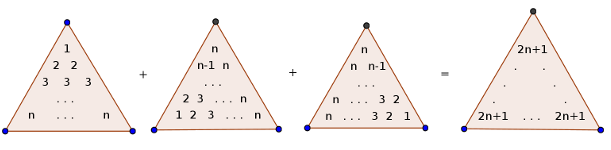
\includegraphics[width=\textwidth]{figure/triangle-proof.png}
\end{minipage}

На языке формул:
\[
  3S = (2n+1) \cdot (1 + 2 + \ldots + n) = (2n+1)n\frac{n+1}{2}.
\]
\end{solution}
\protect \hypertarget {soln:21.2}{}
\begin{solution}{{21.2}}
  Проекцией вектора $(6, 3, 7, 8, 9, 10, 11)$; $a=6$, $b=5$, $c= 9$;
\end{solution}
\protect \hypertarget {soln:21.3}{}
\begin{solution}{{21.3}}
\end{solution}
\protect \hypertarget {soln:21.4}{}
\begin{solution}{{21.4}}
\begin{enumerate}
\item $\chi^2_d$
\item $d$
\item $2d$
\item $\chi^2_{a+b}$
\end{enumerate}
\end{solution}
\protect \hypertarget {soln:21.5}{}
\begin{solution}{{21.5}}
  $Q= Z_1^2$, зная функцию плотности $Z_1$, $f(z_1) = \frac{1}{\sqrt{2\pi}}\exp(-z_1^2/2)$, находим функцию плотности $Q$;
\end{solution}
\protect \hypertarget {soln:21.6}{}
\begin{solution}{{21.6}}
\end{solution}
\protect \hypertarget {soln:21.7}{}
\begin{solution}{{21.7}}
\end{solution}
\protect \hypertarget {soln:21.8}{}
\begin{solution}{{21.8}}
  $\hat Z = \langle Z, z\rangle \cdot v$;
$\hat Z_i = \langle Z, z\rangle \cdot v_i$;
$\Var(\langle Z, z\rangle)=1$; $\Cov(\hat Z_i, \hat Z_j)=v_i v_j \Var( \langle Z, z\rangle)= v_i v_j$;
\end{solution}
\protect \hypertarget {soln:22.1}{}
\begin{solution}{{22.1}}
  Метод максимального правдоподобия:
  \[
    C_n^{Y_{\text{к}}}C_{n-Y_{\text{к}}}^{Y_{\text{щ}}}a^{Y_{\text{к}}}(2a)^{Y_{\text{щ}}}(1-3a)^{Y_{\text{б}}} \to \max_a
  \]
Решая задачу максимизации Кота Матроскина получаем
\[
\hat a_{КМ} = \frac{Y_{\text{к}} + Y_{\text{щ}}}{3n}
\]

Замечаем, что $Y_{\text{к}} + Y_{\text{щ}} \sim Bin(n, 3a)$. Отсюда $\E(\hat a_{\text{КМ}})=a$, $\Var(\hat a_{\text{КМ}}) = \frac{a(1-3a)}{n}$. Оценка несмещённая и состоятельная.

С точки зрения Пса Шарика, неизвестными являются две вероятности, $a$ и $b$. Он решает задачу максимизации по двум переменным. В результате получается вполне себе интуитивная оценка $\hat a_{\text{ПШ}} = Y_{\text{к}}/n$.

\end{solution}
\protect \hypertarget {soln:22.2}{}
\begin{solution}{{22.2}}
Метод правдоподобия: $\max_n \P(S=80)$. Замечаем, что $S \sim Bin\left(100, p=\frac{100}{n}\right)$. Отсюда, $\hat n_{ML} = 125$.

Метод моментов. Рассмотрим $Y_1$, $Y_2$, \ldots, $Y_n$. Величина $Y_i$ равна 1 если при втором отлове $i$-ый заяц оказался с бантом и 0 иначе.

Метод моментов: $\E(Y_i)|_{n=\hat n}=\bar Y$:
\[
\frac{100}{\hat n_{MM}}=\bar Y
\]
Отсюда
\[
\hat n_{MM} = \frac{100}{\bar Y} = \frac{100^2}{S}
\]
\end{solution}
\protect \hypertarget {soln:22.3}{}
\begin{solution}{{22.3}}
\end{solution}
\protect \hypertarget {soln:22.4}{}
\begin{solution}{{22.4}}
\end{solution}
\protect \hypertarget {soln:22.5}{}
\begin{solution}{{22.5}}
\end{solution}
\protect \hypertarget {soln:23.1}{}
\begin{solution}{{23.1}}
  $\hat{\theta}_{ML}=0.25$, $\hat{\theta}_{MM}=0.2$
  $\hat{\theta}_{MM}=\frac{2{,}4-\bar{X}}{7}$
\end{solution}
\protect \hypertarget {soln:23.2}{}
\begin{solution}{{23.2}}
$\hat{a}=\ln(Y_{1})$, $\hat{b}=\ln(Y_{2})-\ln(Y_{1})$
\end{solution}
\protect \hypertarget {soln:23.3}{}
\begin{solution}{{23.3}}
\end{solution}
\protect \hypertarget {soln:23.4}{}
\begin{solution}{{23.4}}
\end{solution}
\protect \hypertarget {soln:23.5}{}
\begin{solution}{{23.5}}
\end{solution}
\protect \hypertarget {soln:23.6}{}
\begin{solution}{{23.6}}
$\hat{a}_{ml}=\sum X_i^2/2n$, $\hat{a}_{mm}=\bar{X}$.
\end{solution}
\protect \hypertarget {soln:23.7}{}
\begin{solution}{{23.7}}
\end{solution}
\protect \hypertarget {soln:23.8}{}
\begin{solution}{{23.8}}
\end{solution}
\protect \hypertarget {soln:23.9}{}
\begin{solution}{{23.9}}
\end{solution}
\protect \hypertarget {soln:23.10}{}
\begin{solution}{{23.10}}
\end{solution}
\protect \hypertarget {soln:23.11}{}
\begin{solution}{{23.11}}
\end{solution}
\protect \hypertarget {soln:23.12}{}
\begin{solution}{{23.12}}
\end{solution}
\protect \hypertarget {soln:23.13}{}
\begin{solution}{{23.13}}
\end{solution}
\protect \hypertarget {soln:23.14}{}
\begin{solution}{{23.14}}
\end{solution}
\protect \hypertarget {soln:23.15}{}
\begin{solution}{{23.15}}
\end{solution}
\protect \hypertarget {soln:23.16}{}
\begin{solution}{{23.16}}
\end{solution}
\protect \hypertarget {soln:23.17}{}
\begin{solution}{{23.17}}
\end{solution}
\protect \hypertarget {soln:23.18}{}
\begin{solution}{{23.18}}
\end{solution}
\protect \hypertarget {soln:23.19}{}
\begin{solution}{{23.19}}
\end{solution}
\protect \hypertarget {soln:23.20}{}
\begin{solution}{{23.20}}
\end{solution}
\protect \hypertarget {soln:23.21}{}
\begin{solution}{{23.21}}
\begin{enumerate}
\item $\E(X_i) = a$, $\E(|X_i|) = 5a/4$
\item $\hat a = 11/30$
\item $\hat a = 26/75$
\item $\hat{a}_{GMM} = 108/325$
\item $\begin{pmatrix}
37 & -44 \\
-44 & 64
\end{pmatrix}$
\end{enumerate}
\end{solution}
\protect \hypertarget {soln:23.22}{}
\begin{solution}{{23.22}}
\end{solution}
\protect \hypertarget {soln:23.23}{}
\begin{solution}{{23.23}}
  $\plim_{n\to\infty} \hat\alpha_{ML}(n) = 0$, не является состоятельной
\end{solution}
\protect \hypertarget {soln:23.24}{}
\begin{solution}{{23.24}}

\end{solution}
\protect \hypertarget {soln:24.1}{}
\begin{solution}{{24.1}}
    \begin{enumerate}
      \item $c=1/n$, да
      \item $c=1/(n+\sigma^2/\mu^2)$, нет, так как $\mu$ и $\sigma$ неизвестны
      \item $\lambda=0$ и $\lambda=\sigma^2/\mu^2$
    \end{enumerate}
  
\end{solution}
\protect \hypertarget {soln:24.2}{}
\begin{solution}{{24.2}}
    \begin{enumerate}
    \item несмещённая, состоятельная, линейная, неэффективная
    \item несмещённая, состоятельная, линейная, неэффективная
    \item несмещённая, несостоятельная, линейная, неэффективная
    \item смещённая, состоятельная, линейная
    \item смещённая, состоятельная, нелинейная
    \item несмещённая, состоятельная, линейная, неэффективная
    \item несмещённая, состоятельная, линейная, эффективная
    \item смещённая, несостоятельная, линейная
    \item смещённая, несостоятельная, нелинейная
    \item несмещённая, состоятельная, линейная, неэффективная
    \end{enumerate}
  
\end{solution}
\protect \hypertarget {soln:24.3}{}
\begin{solution}{{24.3}}
\begin{enumerate}
\item $\hat\theta_{ML} = \max\{ Y_1, Y_2, \ldots, Y_n\}$.
\item Все $Y_i$ меньше $\theta$, значит и $\hat\theta$ всегда меньше $\theta$, значит смещённая.
\item $F_{\hat\theta}(t) = \P(\hat\theta \leq t) = \P(Y_1 \leq t, Y_2 \leq t, \ldots) = (\P(Y_1 \leq t))^n$, $\P(Y_1 \leq t) = t^5/\theta^5$, $f_{\hat\theta}(t) = dF_{\hat\theta}(t)/dt = \frac{5n t^{5n-1}}{\theta^{5n}}$.
\item $\E(\hat\theta) = \frac{5n}{5n+1}\theta$.
\item $\hat\theta_{unbiased} = \frac{5n+1}{5n}\hat\theta$.
\end{enumerate}
\end{solution}
\protect \hypertarget {soln:24.4}{}
\begin{solution}{{24.4}}
\begin{enumerate}
  \item $\hat p$ несмещённая
  \item $\sigma^2 = n p(1-p)$.
  \item $\E(\hat\sigma^2) = (n-1)p(1-p)$, смещённая, $\hat\sigma^2_{unbiased} = \frac{n}{n-1} \hat\sigma^2$.
\end{enumerate}
\end{solution}
\protect \hypertarget {soln:24.5}{}
\begin{solution}{{24.5}}

\end{solution}
\protect \hypertarget {soln:24.6}{}
\begin{solution}{{24.6}}

\end{solution}
\protect \hypertarget {soln:24.7}{}
\begin{solution}{{24.7}}

\end{solution}
\protect \hypertarget {soln:24.8}{}
\begin{solution}{{24.8}}

\end{solution}
\protect \hypertarget {soln:24.9}{}
\begin{solution}{{24.9}}

\end{solution}
\protect \hypertarget {soln:24.10}{}
\begin{solution}{{24.10}}

\end{solution}
\protect \hypertarget {soln:24.11}{}
\begin{solution}{{24.11}}

\end{solution}
\protect \hypertarget {soln:24.12}{}
\begin{solution}{{24.12}}
  Закон распределения $X$ также экспоненциальный, но с другим $\lambda$. Честно находим $\E(X)=\theta/20$, отсюда
  $\hat\theta_{unbiased} = 20X$.
\end{solution}
\protect \hypertarget {soln:24.13}{}
\begin{solution}{{24.13}}

\end{solution}
\protect \hypertarget {soln:24.14}{}
\begin{solution}{{24.14}}
Обе оценки несмещённые, состоятельные. Более эффективна $\hat{\beta}_{2}=\frac{\sum{x_{i}Y_{i}}}{\sum x_{i}^{2}}$.
\end{solution}
\protect \hypertarget {soln:24.15}{}
\begin{solution}{{24.15}}

\end{solution}
\protect \hypertarget {soln:25.1}{}
\begin{solution}{{25.1}}
  $\frac{1}{1.8} - \frac{1}{2.2}$, $[0;10X]$.
\end{solution}
\protect \hypertarget {soln:25.2}{}
\begin{solution}{{25.2}}
\end{solution}
\protect \hypertarget {soln:25.3}{}
\begin{solution}{{25.3}}
\end{solution}
\protect \hypertarget {soln:25.4}{}
\begin{solution}{{25.4}}
\end{solution}
\protect \hypertarget {soln:25.5}{}
\begin{solution}{{25.5}}
\end{solution}
\protect \hypertarget {soln:25.6}{}
\begin{solution}{{25.6}}
Важна при обоих доверительных интервалах. Без предпосылки о нормальности интервал для дисперсии по данным формулам нельзя построить даже при больших $n$. При больших $n$ можно отказаться от предпосылки о нормальности при построении интервала для $\mu$.
\end{solution}
\protect \hypertarget {soln:25.7}{}
\begin{solution}{{25.7}}
\end{solution}
\protect \hypertarget {soln:26.1}{}
\begin{solution}{{26.1}}
к 1/2
\end{solution}
\protect \hypertarget {soln:26.2}{}
\begin{solution}{{26.2}}
  равномерно, $\alpha=0.05$; нет, он резко увеличивает ошибку второго рода
\end{solution}
\protect \hypertarget {soln:26.3}{}
\begin{solution}{{26.3}}
  $\alpha = 1/8$, $\beta = 9/32$
\end{solution}
\protect \hypertarget {soln:26.4}{}
\begin{solution}{{26.4}}
  $\alpha = \P(\cN(0;1) > -0.35) \approx 0.64$, $\beta = \P(\cN(0;1) \leq -1.76) \approx 0.04$.
\end{solution}
\protect \hypertarget {soln:26.5}{}
\begin{solution}{{26.5}}
\end{solution}
\protect \hypertarget {soln:26.6}{}
\begin{solution}{{26.6}}
\end{solution}
\protect \hypertarget {soln:26.7}{}
\begin{solution}{{26.7}}

\end{solution}
\protect \hypertarget {soln:26.8}{}
\begin{solution}{{26.8}}
Критерий Неймана-Пирсона сводится к сравнению $\bar X$ с порогом. При верной $H_0$ величина $\bar X$ распределена $\cN(0; \frac{4}{n})$.
Отсюда искомый критерий имеет вид:
Если $\bar X  \geqslant 0.825$, то гипотеза ${H_0}$ отвергается в пользу гипотезы ${H_a}$.
\end{solution}
\protect \hypertarget {soln:26.9}{}
\begin{solution}{{26.9}}
  Упрощая неравенство из леммы Неймана-Пирсона, получаем критерий: если $X_1\cdot X_2 >t$, то $H_0$ отвергается. Величину $t$ находим из уравнения
\[
\int_0^t (1 - t/x) \, dx = 0.05
\]
\end{solution}
\protect \hypertarget {soln:26.10}{}
\begin{solution}{{26.10}}

\end{solution}
\protect \hypertarget {soln:26.11}{}
\begin{solution}{{26.11}}
\end{solution}
\protect \hypertarget {soln:27.1}{}
\begin{solution}{{27.1}}
При $p_N$ заданном в $H_0$ критерий Пирсона имеет хи-квадрат распределение с двумя степенями свободы.
При оцениваемом $p_N$ критерий Пирсона имеет хи-квадрат распределение с одной степенью свободы.

\url{https://ru.wikipedia.org/wiki/Закон_Харди_—_Вайнберга}
  
\end{solution}
\protect \hypertarget {soln:28.1}{}
\begin{solution}{{28.1}}
$\E(Ay)=A\E(y)$, $\Var(Ay)=A\Var(y)A^T$
\end{solution}
\protect \hypertarget {soln:28.2}{}
\begin{solution}{{28.2}}

\end{solution}
\protect \hypertarget {soln:28.3}{}
\begin{solution}{{28.3}}

\end{solution}
\protect \hypertarget {soln:28.4}{}
\begin{solution}{{28.4}}

\end{solution}
\protect \hypertarget {soln:28.5}{}
\begin{solution}{{28.5}}

\end{solution}
\protect \hypertarget {soln:28.6}{}
\begin{solution}{{28.6}}

\end{solution}
\protect \hypertarget {soln:29.1}{}
\begin{solution}{{29.1}}
Вычтем $2x^2 + 2y^2 + 2z^2 + 2w^2$. Получим, что оптимальное $x=0$. Далее, $z=0$, $y=0$. В итоге $w=1$ или $w=-1$.
\end{solution}
\protect \hypertarget {soln:29.2}{}
\begin{solution}{{29.2}}
\end{solution}
\protect \hypertarget {soln:29.3}{}
\begin{solution}{{29.3}}
\end{solution}
\protect \hypertarget {soln:29.4}{}
\begin{solution}{{29.4}}
\end{solution}
\protect \hypertarget {soln:29.5}{}
\begin{solution}{{29.5}}
$(5+4+1)=10$; длины — $\sqrt{5}\cdot\sqrt{99}$, $\sqrt{4}\cdot\sqrt{99}$, $\sqrt{1}\cdot\sqrt{99}$; выборочные дисперсии — $5$, $4$, $1$; $(5+4)/10=0.9$.
\end{solution}
\protect \hypertarget {soln:29.6}{}
\begin{solution}{{29.6}}
\end{solution}
\protect \hypertarget {soln:30.1}{}
\begin{solution}{{30.1}}
  
\end{solution}
\protect \hypertarget {soln:30.2}{}
\begin{solution}{{30.2}}
  
\end{solution}
\protect \hypertarget {soln:30.3}{}
\begin{solution}{{30.3}}
  
\end{solution}
\protect \hypertarget {soln:31.1}{}
\begin{solution}{{31.1}}
$C_{20}^2\cdot 18$.
\end{solution}
\protect \hypertarget {soln:31.2}{}
\begin{solution}{{31.2}}
  $1+x+x^2+x^3+x^4=(1-x^5)/(1-x)$
  $1+x+x^2+x^3+\ldots = 1/(1-x)$
  $(1+x)^4$
\end{solution}
\protect \hypertarget {soln:31.3}{}
\begin{solution}{{31.3}}
\end{solution}
\protect \hypertarget {soln:31.4}{}
\begin{solution}{{31.4}}
\end{solution}
\protect \hypertarget {soln:31.5}{}
\begin{solution}{{31.5}}
  0 с вероятностью 1/4 и 1 с вероятностью 3/4
\end{solution}
\protect \hypertarget {soln:31.6}{}
\begin{solution}{{31.6}}
  да, сможет!
\end{solution}
\protect \hypertarget {soln:31.7}{}
\begin{solution}{{31.7}}
$F_n = F_{n-1} + F_{n-2}$.
Запишем разложения для $g(x)$, $xg(x)$ и $x^2 g(x)$ друг под другом. Вычитаем. Получаем, что $g(x) = x/(1-x-x^2)$.

Указанная дробь — это и есть производящая функция при маленьком $x$.

Производящая функция представима в виде суммы:
\[
g(x) = \frac{1}{\sqrt{5}}\left( \frac{a}{x+a} - \frac{b}{x+b}  \right),
\]
где $a=(1-\sqrt{5})/2$, $b=(1+\sqrt{5})/2$.
\end{solution}
\protect \hypertarget {soln:31.8}{}
\begin{solution}{{31.8}}
Замечаем, что $h_2(t)=h_1(t)\cdot h_1(t)$. После первого шага:
\[
h_1(t) = 0.7t + 0.3th^2_1(t)
\]
\end{solution}
\protect \hypertarget {soln:31.9}{}
\begin{solution}{{31.9}}

\end{solution}
\protect \hypertarget {soln:32.1}{}
\begin{solution}{{32.1}}
\end{solution}
\protect \hypertarget {soln:32.2}{}
\begin{solution}{{32.2}}
\end{solution}
\protect \hypertarget {soln:33.1}{}
\begin{solution}{{33.1}}
  Если величина $X$ равновероятно принимает $k$ значений, то спутанность равна $k$. У равномерной на $[0;a]$ спутанность равна $a$.
\end{solution}
\protect \hypertarget {soln:33.2}{}
\begin{solution}{{33.2}}
\end{solution}
\protect \hypertarget {soln:33.3}{}
\begin{solution}{{33.3}}
\end{solution}
\protect \hypertarget {soln:33.4}{}
\begin{solution}{{33.4}}
\end{solution}
\protect \hypertarget {soln:33.5}{}
\begin{solution}{{33.5}}
\end{solution}


\section{Источники мудрости}
\printbibliography[heading=none]


\end{document}
